%%%%%%%%%%%%%%%%%%%%%%%%%%%%%%%%%%%%%%%%%%%%%%%%%%%%%%%%%%%%%%%%%%%%%%
% Lớp 11 | Đường thẳng, mặt phẳng. Quan hệ song song trong | Đường thẳng và mặt phẳng song song
% Dạng 1H4?3-3: Tìm giao tuyến bằng cách kẻ song song
% Số câu: 82  (sinh tự động bởi tach_cau.py; từ nay thầy sửa trực tiếp file này)
%%%%%%%%%%%%%%%%%%%%%%%%%%%%%%%%%%%%%%%%%%%%%%%%%%%%%%%%%%%%%%%%%%%%%%

%%%%%%%%%%%%%%%% TRẮC NGHIỆM 4 PHƯƠNG ÁN %%%%%%%%%%%%%%%%

% nguồn: Ok_Toan11_TracNghiem_Lan2
\begin{ex}%[1H4N3-3]%[ma:8bb80cdb]
	Cho hình chóp $S.ABCD$ có mặt đáy $ABCD$  là hình bình hành. Gọi đường thẳng $d$ là giao tuyến của hai mặt phẳng $(SAD)$ và $(SBC)$. Khẳng định nào sau đây đúng?
	 \choice
		{Đường thẳng $d$ đi qua $S$ và  song song với $AB$}
		{Đường thẳng $d$ đi  qua $S$ và song song với $DC$}
		{\True Đường thẳng $d$ đi qua $S$ và song song với  $BC$}
		{Đường thẳng $d$  đi qua $S$ và song song với $BD$}
	\loigiai{ 
		\begin{center}
			\begin{tikzpicture}[scale=.7,font=\footnotesize,line join=round,line cap=round,>=stealth]
					\coordinate (A)  at (0,0);
					\coordinate (B) at (-2,-2); 
					\coordinate (C)  at (4,-2);
					\coordinate (D) at  (6,0);
					\coordinate  (S) at ($(A)+(1,4)$);
					 \coordinate (M) at ($(S)+(D)$);
					 \coordinate (N) at ($(S)+(-3,0)$);
					\draw (S)--(B)--(C)--(S)--(D)--(C) 
						 (M)--(N) node[above]{$d$};
					\draw[dashed] (B)--(A)--(D) 
						(A)--(S); 
					\foreach \p/\g in {A/135,B/-135,C/-45,D/45,S/90}\draw[fill=black] (\p)  circle (1pt) node[shift={(\g:.3)}]{$\p$};
				\end{tikzpicture}
		\end{center}
		Ta có $\heva{&S\in(SAD)\cap(SBC)\\&AD\subset(SAD)\\&BC\subset(SBC)\\&AD \parallel BC}\Rightarrow (SAD)\cap(SBC)=d$ ($d$ đi qua $S$ và song song với $BC$,  $AD$).
	 }
\end{ex}

% nguồn: Ok_Toan11_TracNghiem_Lan2
\begin{ex}%[1H4N3-3]%[ma:88e50bcb]
	Cho hình chóp $S.ABCD$ có đáy  $ABCD$ là hình thang, $AD \parallel BC$. Giao tuyến của $(SAD)$ và $(SBC)$ là
	\choice 
		{Đường thẳng đi  qua $S$ và song song với $AB$}
		{Đường thẳng đi qua $S$ và song  song với $CD$}
		{Đường thẳng đi qua $S$ và song  song với $AC$}
		{\True Đường thẳng đi  qua $S$ và song song với $AD$}
	 \loigiai{
		\begin{center}
			\begin{tikzpicture}[scale=.7,font=\footnotesize,line join=round,line cap=round,>=stealth]
					\coordinate (A)  at (0,0);
					\coordinate (B)  at (1,-2);
					 \coordinate (C) at (4,-2);
					 \coordinate (D) at (6,0);
					\coordinate  (S) at ($(A)+(1,4)$);
					\coordinate (M)  at ($(S)+(D)$);
					\coordinate (N)  at ($(S)+(-3,0)$);
					\draw  (S)--(B)--(C)--(S)--(D)--(C)
						 (S)--(A)--(B)
						 (M)--(N) node[above]{$d$};
					\draw[dashed] (A)--(D); 
					\foreach  \p/\g in {A/135,B/-135,C/-45,D/45,S/90}\draw[fill=black] (\p) circle (1pt) node[shift={(\g:.3)}]{$\p$};
				\end{tikzpicture}
		\end{center}
		Hai mặt phẳng $(SAD)$ và $(SBC)$ có một điểm chung là $S$ và lần lượt chứa hai đường thẳng $AD$ và  $BC$ song song nhau nên giao tuyến $d$ của hai mặt phẳng $(SAD)$ và $(SBC)$ đi qua $S$ và song song $AD$, $BC$.
	} 
\end{ex}

% nguồn: Ok_Toan11_TracNghiem_Lan2
\begin{ex}%[1H4N3-3]%[ma:9f44bc4e]
	Cho hình chóp $S.ABCD$ có đáy là hình bình hành. Gọi $I$, $J$ lần lượt là trung điểm của $AB$ và $CB$. Khi đó giao tuyến của 2 mặt phẳng $(SAB)$ và $(SCD)$ là đường thẳng song song với 
	\choice 
		{$AD$} 
		 {$IJ$}
		{$BJ$} 
		{\True  $BI$}
	\loigiai{ 
		\begin{center}
			\begin{tikzpicture}[scale=.7,font=\footnotesize,line join=round,line cap=round,>=stealth]
					\coordinate (C) at (0,0); 
					\coordinate (B)  at (-2,-2);
					\coordinate (A)  at (4,-2);
					\coordinate (D) at (6,0); 
					\coordinate (S) at ($(C)+(.5,4)$); 
					 \coordinate (M) at ($(S)+(D)$);
					\coordinate  (J) at ($(B)!.5!(C)$);
					\coordinate (I) at ($(A)!.5!(B)$); 
					 \draw (S)--(B)--(A)--(D)--(S)--(A)
						 (S)--(M) node[above]{$d$};
					\draw[dashed] (B)--(C)--(D) 
						 (C)--(S);
					\foreach \p/\g in {C/135,B/-135,A/-45,D/45,S/90,I/-90,J/0}\draw[fill=black]  (\p) circle (1pt) node[shift={(\g:.3)}]{$\p$};
				\end{tikzpicture}
		\end{center}
		Gọi $d$ là đường thẳng qua $S$ và song song  với $AB\Rightarrow d \parallel BI$.\\
		Ta  có $\heva{&AB \parallel CD\\&AB\subset(SAB)\\&CD\subset(SCD)}\Rightarrow(SAB)\cap(SCD)=d$.\\
		Vậy giao tuyến cần tìm song  song với $BI$.
	 }
\end{ex}

% nguồn: Ok_Toan11_TracNghiem_Lan2
\begin{ex}%[1H4N3-3]%[ma:2194a808]
	Cho hình chóp $S.ABCD$ có đáy là hình bình hành. Giao tuyến của $(SAB)$ và  $(SCD)$ là
	\choice 
		{Đường  thẳng qua $S$ và song song với $AD$}
		{\True Đường thẳng qua $S$  và song song với $CD$}
		{Đường $SO$ với $O$ là tâm hình bình hành} 
		{Đường thẳng  qua $S$ và cắt $AB$}
	\loigiai{ 
		\begin{center}
			\begin{tikzpicture}[scale=.7,font=\footnotesize,line join=round,line cap=round,>=stealth]
					 \coordinate (A) at (0,0);
					\coordinate (D)  at (-2,-2);
					\coordinate  (C) at (4,-2);
					 \coordinate (B) at (6,0);
					\coordinate (S) at ($(A)+(.5,4)$); 
					\coordinate (M) at  ($(S)+(B)$);
					\draw (S)--(B)--(C)--(S)--(D)--(C) 
						(S)--(M)  node[above]{$t$};
					\draw[dashed]  (B)--(A)--(D)
						(A)--(S); 
					 \foreach \p/\g in {A/135,D/-135,C/-45,B/45,S/90}\draw[fill=black] (\p) circle (1pt) node[shift={(\g:.3)}]{$\p$};
				\end{tikzpicture}
		\end{center}
		Ta có $\heva{&S\in (SAB)  \cap (SCD)\\&AB\subset(SAB)\\&CD\subset(SCD)\\&AB \parallel CD}$, suy ra giao tuyến của hai mặt phẳng $(SAB)$ và $(SCD)$ là đường thẳng $St$ đi qua điểm $S$ và song song với $CD$.
	 }
\end{ex}

% nguồn: Ok_Toan11_TracNghiem_Lan2
\begin{ex}%[1H4N3-3]%[ma:71bb763d]
	Cho hình chóp  $S.ABCD$ có đáy $ABCD$ là hình bình hành. Tìm giao tuyến của hai mặt phẳng $(SAD)$ và $(SBC)$.
	\begin{center}
		\begin{tikzpicture}[scale=.7,font=\footnotesize,line join=round,line cap=round,>=stealth]
				\path 
					(0,0) coordinate (A) 
					 (5,0) coordinate (B)
					(-2.5,-1.5) coordinate  (D)
					(1,3.5) coordinate  (S)
					($(B)+(D)-(A)$) coordinate  (C);
				\draw  (S)--(D)--(C)--(B)--(S)--(C);
				\draw [dashed]  (S)--(A)--(B)
					(A)--(D); 
				\foreach \d/\g in {A/135,D/-135,C/-45,B/45,S/90} 
				\fill (\d) circle (1pt) + (\g:.3) node{$\d$}; 
			\end{tikzpicture}
	\end{center}
	\choice 
		{Là đường thẳng đi qua đỉnh $S$ và tâm  $O$ của đáy}
		{\True Là đường thẳng đi qua  đỉnh $S$ và song song với đường thẳng $BC$}
		{Là đường thẳng đi qua đỉnh $S$ và  song song với đường thẳng $AB$}
		{Là đường thẳng đi qua đỉnh $S$ và song song với đường thẳng  $BD$}
	\loigiai{ 
		\begin{center}
			\begin{tikzpicture}[scale=1,font=\footnotesize,line join=round,line cap=round,>=stealth]
					\path 
						(0,0) coordinate  (A)
						 (5,0) coordinate (B)
						(-2.5,-1.5) coordinate (D) 
						(1,3.5)  coordinate (S)
						 ($(B)+(D)-(A)$) coordinate (C)
						($(S)+(B)-(C)$) coordinate (d) 
						($(d)!2!(S)$) coordinate (K); 
					\draw  (S)--(D)--(C)--(B)--(S)--(C)
						 (d)--(K);
					\draw [dashed] (S)--(A)--(B) 
						(A)--(D); 
					\foreach  \d/\g in {A/135,D/-135,C/-45,B/45,S/90}
					\fill (\d) circle (1pt) + (\g:.3)  node{$\d$};
				\end{tikzpicture}
		\end{center}
		Do hai mặt phẳng $(SAD)$ và $(SBC)$ có chung điểm $S$ và có hai  đường thẳng $AD$, $BC$ song song với nhau nên giao tuyến của hai mặt phẳng $(SAD)$ và $(SBC)$ là đường thẳng đi qua đỉnh $S$ và song song với đường thẳng $BC$.
	 }
\end{ex}

% nguồn: Ok_Toan11_TracNghiem_Lan2
\begin{ex}%[1H4N3-3]%[ma:d4fd4177]
	Cho hình chóp  $S.ABCD$ có đáy là hình thang $ABCD$ ($AB \parallel CD$). Gọi $E$, $F$ lần lượt là trung điểm của $AD$ và $BC$. Giao tuyến của hai mặt phẳng $(SAB)$ và $(SCD)$ là
	\choice 
		{Đường thẳng đi qua $S$ và qua giao  điểm của cặp đường thẳng $AB$ và $SC$}
		{Đường  thẳng đi qua $S$ và song song với $AD$}
		{Đường thẳng đi qua $S$  và song song với $AF$}
		{\True Đường thẳng đi  qua $S$ và song song với $EF$}
	 \loigiai{
		\begin{center}
			\begin{tikzpicture}[scale=.7,font=\footnotesize,line join=round,line cap=round,>=stealth]
					\coordinate  (A) at (0,0);
					\coordinate (D)  at (1,-2);
					\coordinate (C)  at (4,-2);
					\coordinate (B) at (6,0); 
					\coordinate (S)  at ($(A)+(1,4)$);
					\coordinate (M) at ($(S)+(4,0)$); 
					\coordinate (N) at  ($(S)+(-3,0)$);
					\coordinate (E) at ($(A)!.5!(D)$); 
					 \coordinate (F) at ($(B)!.5!(C)$);
					\draw  (S)--(D)--(C)--(S)--(B)--(C)
						 (S)--(A)--(D)
						(M)--(N)  node[above]{$d$};
					 \draw[dashed] (A)--(B)
						(E)--(F); 
					\foreach \p/\g in {A/135,D/-135,C/-45,B/45,S/90,E/180,F/0}\draw[fill=black] (\p)  circle (1pt) node[shift={(\g:.3)}]{$\p$};
				\end{tikzpicture}
		\end{center}
		 Ta có $\heva{&AB \parallel CD\\&AB\subset(SAB)\\&CD\subset(SCD)}\Rightarrow (SAB)\cap(SCD)=d$ ($d$ đi qua $S$ và song song với $AB$)\\
		Lại có $AB \parallel EF$, nên giao tuyến của hai mặt phẳng  $(SAB)$ và $(SCD)$ là đường thẳng $d$ đi qua $S$ và song song với $EF$.
	} 
\end{ex}

% nguồn: Ok_Toan11_TracNghiem_Lan2
\begin{ex}%[1H4N3-3]%[ma:8b9a1440]
	Cho hình chóp $S.ABCD$, đáy $ABCD$ là hình bình hành. Giao tuyến của hai mặt phẳng $(SAD)$  và $(SBC)$ là đường thẳng song song với đường thẳng nào sau đây?
	 \choice
		{\True  $AD$}
		 {$AC$}
		 {$DC$}
		{$BD$} 
	 \loigiai{
		\begin{center}
			\begin{tikzpicture}[scale=.7,font=\footnotesize,line join=round,line cap=round,>=stealth]
					\coordinate  (A) at (0,0);
					 \coordinate (B) at (-2,-2);
					\coordinate  (C) at (4,-2);
					 \coordinate (D) at (6,0);
					\coordinate (S) at ($(A)+(1,4)$); 
					\coordinate (M) at ($(S)+(D)$); 
					\coordinate (N) at  ($(S)+(-3,0)$);
					\draw  (S)--(B)--(C)--(S)--(D)--(C)
						(M)--(N)  node[above]{$d$};
					 \draw[dashed] (B)--(A)--(D)
						(A)--(S); 
					\foreach \p/\g in {A/135,B/-135,C/-45,D/45,S/90}\draw[fill=black] (\p) circle (1pt)  node[shift={(\g:.3)}]{$\p$};
				\end{tikzpicture}
		\end{center}
		 Ta có $AD \parallel BC\Rightarrow(SAD)\cap(SBC)=d$, với $d$ là đường thẳng đi qua $S$ và song song với $AD$
	 }
\end{ex}

% nguồn: Ok_Toan11_TracNghiem_Lan2
\begin{ex}%[1H4H3-3]%[ma:f637ecb3]
	Cho tứ diện $ABCD$. $I$ và $J$ theo  thứ tự là trung điểm của $AD$ và $AC$. $G$ là trọng tâm tam giác $BCD$. Giao tuyến của hai mặt phẳng $(GIJ)$ và $(BCD)$ là đường thẳng
	 \choice
		{Qua  $I$ và song song với $AB$}
		 {Qua $J$ và song song với $BD$}
		{\True Qua $G$ và song  song với $CD$}
		{Qua $G$ và song song với $BC$} 
	 \loigiai{
	\immini{Xét hai mặt phẳng  $(GIJ)$ và $(BCD)$, có $G \in (GIJ) \cap (BCD)$. \\
		Mặt khác $IJ \parallel CD$ ($IJ$ là đường trung bình của $\triangle ACD$), $IJ \subset (GJI)$, $CD \subset (BCD)$ nên $(GIJ) \cap (BCD)=Gy$, với $Gy$ là đường thẳng qua $G$ và song song với $CD$.}{\begin{tikzpicture}[line join=round,line cap=round,line width=.6pt,font=\footnotesize,scale=1]
		\coordinate[label=left:$B$] (B) at  (0,0);
		\coordinate[label=below left:$C$] (C) at (1,-2); 
		\coordinate[label=right:$D$]  (D) at (5,0);
		\coordinate[label=above left:$A$] (A) at (1.2,4); 
		\coordinate[label=above  left:$J$] (J) at ($(A)!1/2!(C)$);
		\coordinate[label=above right:$I$]  (I) at ($(A)!1/2!(D)$);
		\coordinate (M) at ($(B)!1/2!(C)$); 
		\coordinate[label=below:$G$]  (G) at ($(D)!2/3!(M)$);
		\coordinate (N)  at ($(B)!2/3!(D)$);
		 \draw (B)--(C)--(D)--(A)--cycle (A)--(C)
			 (I)--(J);
		 \draw[dashed] (B)--(D)--(M)
			(J)--(G)--(I) 
			 (G)--(N);
		\fill  (A) circle (1pt)
			 (B) circle (1pt)
			 (C) circle (1pt)
			(D) circle  (1pt)
			(I) circle  (1pt)
			(J)  circle (1pt)
			(G)  circle (1pt);
	\end{tikzpicture}
	 }}
\end{ex}

% nguồn: Ok_Toan11_TracNghiem_Lan2
\begin{ex}%[1H4H3-3]%[ma:e2398861]
	Cho chóp $S.ABCD$ đáy là hình thang. Gọi $I$, $K$ lần lượt là trung điểm của $AD$, $BG$ là trọng tâm tam giác $SAB$. Khi đó giao tuyến  của 2 mặt phẳng $(IKG)$ và $(SAB)$ là?
	\choice 
		{Giao tuyến $(IKG)$ và $(SAB)$ là đường thẳng đi qua $S$ và  song song $AB$, $IK$}
		{Giao tuyến $(IKG)$ và  $(SAB)$ là đường thẳng đi qua $S$ và song song $AD$}
		{Giao tuyến $(IKG)$ và $(SAB)$ là đường thẳng đi qua $G$ và song song  $CB$}
		{\True Giao tuyến $(IKG)$ và $(SAB)$ là  đường thẳng đi qua $G$ và song song $AB$, $IK$}
	\loigiai{ 
		\begin{center}
			\begin{tikzpicture}[scale=.7,font=\footnotesize,line join=round,line cap=round,>=stealth]
					\coordinate  (A) at (0,0);
					\coordinate (D) at  (2,-2);
					 \coordinate (C) at (5,-2);
					\coordinate (B) at (6,0); 
					\coordinate (S) at  ($(A)+(2,4)$);
					\coordinate (F) at  ($(S)!2/3!(B)$);
					\coordinate (E) at ($(S)!2/3!(A)$); 
					\coordinate (G)  at ($(E)!.5!(F)$);
					\coordinate (I) at ($(A)!.5!(D)$); 
					\coordinate (J) at ($(A)!.5!(B)$); 
					 \coordinate (K) at ($(B)!.5!(C)$);
					\draw (S)--(D)--(C)--(S)--(B)--(C) 
						 (S)--(A)--(D)
						(E)--(I) 
						 (F)--(K);
					 \draw[dashed] (A)--(B)
						(I)--(K) 
						 (F)--(E)
						 (S)--(J);
					\foreach \p/\g  in {A/135,D/-135,C/-45,B/45,S/90,I/180,K/0,G/45,F/30,E/150,J/-90}\draw[fill=black] (\p) circle (1pt) node[shift={(\g:.3)}]{$\p$};
				\end{tikzpicture}
		\end{center}
		Xét hai mặt phẳng  $(IKG)$, $(SAB)$\\
		Ta có $G\in(GIK)$; $G\in(SAB)$ suy ra $G$ là điểm  chung thứ nhất.\\
		$IK \parallel  AB$, $IK\subset(GIK)$, $AB\subset(SAB)$.\\
		Suy ra $(IKG)\cap(SAB)=Gx  \parallel IK \parallel AB$.
	} 
\end{ex}

% nguồn: Ok_Toan11_TracNghiem_Lan2
\begin{ex}%[1H4H3-3]%[ma:40c4a3a5]
	Cho hình chóp $S.ABCD$, đáy $ABCD$ là hình  bình hành. Giao tuyến của hai mặt phẳng ($SAD$) và $(SBC)$ là đường thẳng song song với đường thẳng nào sau đây?
	 \choice
		{$AC$} 
		 {$DC$}
		 {$BD$}
		 {\True $AD$}
	\loigiai{ 
		\begin{center}
			\begin{tikzpicture}[line join = round,line cap = round,>=stealth,font=\footnotesize,scale=1,declare function={ab=2.5; ad=4.5; gs=80; sa=3; gocA=-130;}]
					\path 
						(0,0) coordinate  (A)
						(ad,0) coordinate  (D)
						(gocA:ab)  coordinate (B)
						 ($(D)-(A)+(B)$) coordinate (C)
						(gs:sa) coordinate  (S)
						 ($(D)-(A)+(S)$) coordinate (d);
					\draw[shorten <= -1cm,shorten >= 1cm] (S)--(d)  node[above,pos=0.6,sloped]{$d$};
					 \draw (S)--(B)--(C)--(D)--(S)--(C);
					\draw[dashed]  (S)--(A)--(D)
						 (B)--(A);
					\foreach \x/\gm in {A/150,B/180,C/-20,D/0,S/90} \fill (\x) circle  (1pt)
						($(\x)+(\gm:3.5mm)$) node{$\x$}; 
				\end{tikzpicture}
		\end{center}
		Giao tuyến của 2 mặt phẳng chứa 2 đường thẳng song song với nhau là đường  thẳng đi qua 1 điểm chung của 2 mặt phẳng đó và song song với 2 đường thẳng song song trên.
		Mà $AD\parallel BC$ nên giao tuyến của hai mặt phẳng $(SAD)$ và $(SBC)$ là đường thẳng qua $S$ và song song  với $AD$.
	} 
\end{ex}

% nguồn: Ok_Toan11_TracNghiem_Lan2
\begin{ex}%[1H4H3-3]%[ma:d705f50c]
	Cho tứ diện $ABCD$. Gọi $M$, $N$ lần lượt là trung điểm của $AD$ và $AC$. Gọi $G$ là một điểm thuộc cạnh BC sao cho $BG=2GC$. Giao tuyến của hai mặt phẳng $(GMN)$ và  $(BCD)$ là đường thẳng.
	 \choice
		{\True qua $G$ và  song song với $CD$}
		{qua $G$ và song song với  $BC$}
		{qua $N$ và song song  với $BD$}
		{qua $M$ và song song với  $AB$}
	 \loigiai{
		\begin{center}
			\begin{tikzpicture}[scale=1,font=\footnotesize,line join=round,line cap=round,>=stealth]
					\path 
						(0,0) coordinate (B) 
						(6,0)  coordinate (D)
						(1.8,-2) coordinate (C) 
						 (1.5,3) coordinate (A)
						($(B)!{2/3} !(C)$) coordinate  (G)
						 ($(A)!.5 !(C)$) coordinate (N)
						($(A)!.5!(D)$)  coordinate (M)
						($(B)!{2/3} !(D)$) coordinate (E) 
						 ($(G)!1.25 !(E)$) coordinate (F)
						($(E)!{3/2} !(G)$) coordinate  (K);
					 \draw [dashed] (B)--(D)
						 (M)--(G)
						(G)--(F); 
					 \draw (A)--(B)--(C)--(D)--(A)--(C)
						 (G)--(N)--(M)
						 (G)--(K);
					\foreach \p/\g in {A/90,B/180,C/-90,D/0,M/45,N/190,G/-90}\draw[fill=black] (\p) circle  (1pt) node[shift={(\g:.3)}]{$\p$};
				\end{tikzpicture}
		\end{center}
		Hai mặt phẳng $(GMN)$ và $(BCD)$ lần lượt chứa hai đường thẳng song song là $MN$ và $CD$ nên giao tuyến của chúng là đường thẳng qua $G$ và  song song với $CD$.
	 }
\end{ex}

% nguồn: Ok_Toan11_TracNghiem_Lan2
\begin{ex}%[1H4H3-3]%[ma:0ee7bd11]
	Cho hình chóp $S.ABCD$ có đáy $ABCD$ là hình thang với $AD \parallel BC$. Gọi $M$ là trung điểm của $SC$. Gọi $d$ là giao tuyến của hai mặt phẳng  $(SBC)$ và $(MAD)$. Kết luận nào sau đây \textbf{sai}.
	\choice 
		{$d$  cắt $SB$}
		{$d \parallel AD$} 
		{\True $d$ cắt  $SA$}
		{$d$ và $AC$ chéo nhau} 
	\loigiai{ 
		\begin{center}
			\begin{tikzpicture}[scale=.7,font=\footnotesize,line join=round,line cap=round,>=stealth]
					 \coordinate (A) at (0,0);
					\coordinate (B) at  (1,-2);
					\coordinate (C) at (4,-2); 
					 \coordinate (D) at (6,0);
					 \coordinate (S) at ($(A)+(1,4)$);
					\coordinate (M) at  ($(S)!.5!(C)$);
					 \coordinate (N) at ($(S)!.5!(B)$);
					\coordinate (E)  at ($(M)!1.4!(N)$);
					\coordinate  (F) at ($(N)!1.7!(M)$);
					\draw  (S)--(B)--(C)--(S)--(D)--(C)
						(S)--(A)--(B) 
						(M)--(D) 
						(E)--(F) node[above]{$d$}; 
					 \draw[dashed] (A)--(D)
						(M)--(A); 
					\foreach \p/\g in  {A/135,B/-135,C/-45,D/45,M/45,N/135,S/90}\draw[fill=black] (\p) circle (1pt) node[shift={(\g:.3)}]{$\p$};
				\end{tikzpicture}
		\end{center}
		Ta có $\heva{&M\in(SBC)\cap(MAD)\\&BC \parallel AD\\&d=(SBC)\cap(MAD)}$, suy ra $d$ đi qua $M$ và $d \parallel  AD$, $d \parallel BC$.\\
		Do đó $d$ cắt $SB$, $d$ và $SA$  chéo nhau.
	} 
\end{ex}

% nguồn: Ok_Toan11_TracNghiem_Lan2
\begin{ex}%[1H4H3-3]%[ma:975dfd22]
	Cho hình chóp $S.ABCD$ có đáy $ABCD$ là hình bình hành tâm $O$. Gọi $M$, $N$, $P$, $Q$ lần lượt là trung điểm của các cạnh $AD$, $BC$, $SC$, $SD$. Gọi $(\alpha)$ là mặt phẳng đi  qua $O$ và song song với mặt phẳng $(SAB)$. Giao tuyến của $(\alpha)$ với các mặt phẳng $(SBC)$ và $(SAD)$ lần lượt là
	 \choice
		{$MN$  và $PN$}
		{$MN$ và $PQ$} 
		{$QP$ và $QM$} 
		{\True $NP$ và  $MQ$}
	\loigiai{ 
		\begin{center}
			\begin{tikzpicture}[line join = round,line cap = round,>=stealth,font=\footnotesize,scale=1,declare function={ab=2.5; ad=4.5; gs=80; sa=3; gocA=-130;}]
					\path 
						(0,0) coordinate (A) 
						(ad,0) coordinate (D) 
						(gocA:ab)  coordinate (B)
						($(D)-(A)+(B)$) coordinate  (C)
						(gs:sa)  coordinate (S)
						($(S)!0.5!(C)$) coordinate (P) 
						($(S)!0.5!(D)$) coordinate  (Q)
						 ($(A)!0.5!(D)$) coordinate (M)
						($(B)!0.5!(C)$) coordinate  (N)
						(intersection of A--C and B--D)  coordinate (O);
					\draw  (S)--(B)--(C)--(D)--(S)--(C)
						 (N)--(P)--(Q);
					\draw[dashed]  (S)--(A)--(D)
						(B)--(A) 
						 (N)--(M)--(Q)
						(A)--(C) 
						(B)--(D); 
					\foreach \x/\gm in {A/150,B/180,C/-20,D/0,S/90,N/-90,Q/90,M/-60,P/180,O/-70} \fill (\x)  circle (1pt)
						($(\x)+(\gm:3.5mm)$) node{$\x$}; 
				\end{tikzpicture}
		\end{center}
		 Vì $(\alpha) \parallel(SAB) \Rightarrow(\alpha) \parallel AB;(\alpha) \parallel SB;(\alpha) \parallel SA$.\\
		Vì $M$, $N$, $P$, $Q$ lần lượt là trung điểm của các cạnh $AD$, $BC$, $SC$, $SD$ nên $MN\parallel AB$; $NP\parallel SB$; $MQ\parallel  SA$.\\
		Ta có $\heva{& (\alpha) \parallel AB\\ & AB\subset(ABCD) \\ & O\in(\alpha), O\in(ABCD)}  \Rightarrow(\alpha) \cap(ABCD)=MN$ qua $O$.\\
		$\heva{& (\alpha) \parallel  SB\\ & SB\subset(SBC) \\ & N\in(\alpha), N\in(SBC)} \Rightarrow(\alpha) \cap(SBC)=NP\parallel SB$.\\
		$\heva{& (\alpha)  \parallel SA\\ & SA\subset(SAD) \\ & M\in(\alpha), M\in(SAD)} \Rightarrow(\alpha) \cap(SAD)=MQ\parallel SA$.\\
		Vậy giao tuyến của ($\alpha$) với các mặt phẳng ($SBC$) và $(SAD)$ lần lượt  là $NP$ và $MQ$.
	} 
\end{ex}

% nguồn: Ok_Toan11_TracNghiem_Lan2
\begin{ex}%[1H4H3-3]%[ma:ce9e5bb5]
	Nếu mặt phẳng $(\alpha)$ chứa đường thẳng $a$ và mặt phẳng $(\beta)$ chứa  đường thẳng $b$, sao cho $a\parallel b$. Khi đó giao tuyến của $(\alpha)$ và $(\beta)$ là
	 \choice
		{\True  Đường thẳng $c$ song song với $a$ và $b$}
		{Đường thẳng $c$ song song hoặc trùng với một trong hai đường thẳng $a$ và $b$} 
		{Đường thẳng $c$ trùng với một trong hai đường thẳng  $a$ và $b$}
		{Đường thẳng $c$  cắt hai đường thẳng $a$ và $b$}
	\loigiai{ 
		Đường thẳng  $c$ song song với $a$ và $b$.
	} 
\end{ex}

% nguồn: Ok_Toan11_TracNghiem_Lan2
\begin{ex}%[1H4H3-3]%[ma:477c604b]
	Cho hình chóp $S. ABC$. Gọi $M$ là trung điểm của $SB$, mặt phẳng ($\alpha$) đi qua $M$ và song song với mặt phẳng $(ABC)$ cắt $SA, SC$ lần lượt tại $N, P$. Khẳng  định nào đúng?
	\choice 
		 {$(\alpha)$ không trùng với $(MNP)$}
		{$MP$ cắt $BC$} 
		{$MN$  cắt $AC$}
		{\True $MP\parallel  BC$}
	\loigiai{ 
		\begin{center}
			\begin{tikzpicture}[line join = round,line cap = round,>=stealth,font=\footnotesize,scale=1,declare function={ac=4; ab=2; gocA=-60; ha=3.5;}]
					 \path
						(0,0)  coordinate (A)
						 (ac,0) coordinate (C)
						(gocA:ab)  coordinate (B)
						(50:ha) coordinate  (S)
						($(S)!0.5!(A)$)  coordinate (N)
						($(S)!0.5!(B)$)  coordinate (M)
						($(S)!0.5!(C)$) coordinate  (P);
					 \draw (S)--(A)--(B)--(C)--cycle (S)--(B)
						(N)--(M)--(P); 
					\draw[dashed]  (A)--(C)
						 (N)--(P);
					\foreach \x/\gm in {S/90,A/180,B/-90,C/0,N/150,P/20,M/-30} \fill (\x)  circle (1pt)
						 ($(\x)+(\gm:3.5mm)$) node{$\x$};
				\end{tikzpicture}
		\end{center}
		Theo cách xác định mặt phẳng $(\alpha)$ ta có $MP\parallel  BC$.
	 }
\end{ex}

% nguồn: Ok_Toan11_TracNghiem_Lan2
\begin{ex}%[1H4H3-3]%[ma:f5689265]
	Cho tứ diện $ABCD$. Gọi $I$ và $J$ theo thứ  tự là trung điểm của $AC$, $AD$ và $G$ là trọng tâm tam giác $BCD$. Giao tuyến của hai mặt phẳng $(GIJ)$ và $(BCD)$ là đường thẳng
	\choice 
		{Qua $I$ và song song với $AB$} 
		{Qua $J$  và song song với $BD$}
		{\True Qua $G$ và  song song với $CD$}
		{Qua $G$ và song song với $BC$} 
	\loigiai{ 
		\begin{center}
			\begin{tikzpicture}[scale=1,font=\footnotesize,line join=round,line cap=round,>=stealth]
					\coordinate (B) at (0,0); \coordinate (C) at  (1.5,-2); \coordinate (D) at (6,0);
					 \coordinate (H) at ($(C)!1/2!(D)$); \coordinate (A) at ($(B)+(1,4)$);
					\coordinate (G) at ($(B)!2/3!(H)$); \coordinate (I) at ($(A)!1/2!(C)$); \coordinate (J) at ($(A)!1/2!(D)$); 
					\coordinate  (M) at ($(B)!2/3!(C)$); \coordinate (N) at ($(B)!2/3!(D)$);
					\draw (A)--(B)--(C)--(D)--(A)--(C) 
						(I)--(J); 
					\draw[dashed] (B)--(D) 
						 (I)--(G)--(J)
						(M)--(N)  node[below,pos=0.7]{$d$};
					\foreach \x/\g in {A/90,B/180,C/-90,D/0,I/150,J/60,G/-90} \fill (\x) circle (1pt) 
						($(\x)+(\g:3mm)$) node{$\x$}; 
				\end{tikzpicture}
		\end{center}
		Gọi $d$  là giao tuyến của $(GIJ)$ và $(BCD)$.\\
		Khi đó $\heva{&G \in (GIJ) \cap (BCD)\\& IJ \parallel CD \\&IJ  \subset (GIJ).}$\\
		Suy ra $d$ đi qua $G$ và song song với  $CD$.
	 }
\end{ex}

% nguồn: Ok_Toan11_TracNghiem_Lan2
\begin{ex}%[1H4H3-3]%[ma:b1a0f99f]
	Cho tứ diện $ABCD$ và ba điểm $P$, $Q$, $R$ lần lượt nằm trên cạnh các $AB$, $CD$, $BC$ (không trùng với các đỉnh của tứ diện $ABCD$) sao cho $PR\parallel AC$. Khi đó giao tuyến của hai mặt phẳng  $(PQR)$ và $(ACD)$ song song với đường thẳng nào trong các đường thẳng sau?
	\choice 
		{$BD$} 
		 {$CD$}
		 {$CB$}
		{\True $AC$} 
	 \loigiai{
		\begin{center}
			\begin{tikzpicture}[line join = round,line cap = round,>=stealth,font=\footnotesize,scale=1,declare function={ab=3; bc=2.2; bd=4.5; gocB=-60; gn=70;}]
					 \path
						(0,0) coordinate (B) 
						(gn:ab) coordinate  (A)
						(bd,0) coordinate (D) 
						(gocB:bc) coordinate (C) 
						($(B)!0.4!(A)$) coordinate  (P)
						($(B)!0.4!(C)$) coordinate  (R)
						($(D)!0.3!(A)$)  coordinate (S)
						($(D)!0.3!(C)$)  coordinate (Q);
					\draw (A)--(B)--(C)--(D)--(A)--(C) 
						(P)--(R) 
						(S)--(Q); 
					\draw[dashed] (D)--(B) 
						 (P)--(S)
						 (R)--(Q);
					\foreach \x/\gm in {A/90,B/180,C/-90,D/0,P/180,S/20,Q/-50,R/-100} \fill  (\x) circle (1pt)
						 ($(\x)+(\gm:3.5mm)$) node{$\x$};
				\end{tikzpicture}
		\end{center}
		 Ta có
		$\heva{& Q\in(PQR) \cap(ACD) \\ & PR\subset(PQR) \\ & AC\subset(ACD) \\ & PR\parallel AC}\text{ nên }(PQR) \cap(ACD)=Qx \parallel AC$.\\ 
	Vậy giao tuyến của hai mặt  phẳng $(PQR)$ và $(ACD)$ song song với đường thẳng $AC$.}
\end{ex}

% nguồn: Ok_Toan11_TracNghiem_Lan2
\begin{ex}%[1H4H3-3]%[ma:544d0202]
	Cho hình chóp $S. ABCD$ có đáy là hình thang $ABCD(AB\parallel CD)$. Gọi $O$ là giao điểm của $AC$ và $BD, I$ là giao điểm của $AD$ và $BC$. Khẳng định nào  sau đây \textbf{sai}?
	\begin{center}
		\begin{tikzpicture}[line join = round,line cap = round,>=stealth,font=\footnotesize,scale=1,declare function={ad=2; cd=2; ab=4.5; gs=80; sa=3; gocA=-50;}]
				\path 
					(0,0)  coordinate (A)
					(ab,0) coordinate  (B)
					 (gocA:ad) coordinate (D)
					($(D)+(cd,0)$)  coordinate (C)
					(gs:sa) coordinate  (S)
					(intersection  of A--D and B--C) coordinate (I)
					 (intersection of A--C and B--D) coordinate (O);
				\draw  (S)--(A)--(D)--(C)--(B)--(S)--(C)
					 (S)--(D)--(I)--(C);
				\draw[dashed]  (B)--(A)
					(A)--(C) 
					 (B)--(D);
				\foreach  \x/\gm in {A/180,B/0,C/-90,D/-90,S/90,I/-90,O/90} \fill (\x) circle (1pt)
					($(\x)+(\gm:3.5mm)$)  node{$\x$};
			\end{tikzpicture}
	\end{center}
	\choice 
		{Giao tuyến của hai mặt phẳng $(SAC)$ và  $(SBC)$ là $SC$}
		{Giao tuyến của hai mặt phẳng ($SAC$) và  ($SBD$) là $SO$}
		{Giao tuyến của hai mặt phẳng $(SAD)$ và $(SBC)$  là $SI$}
		{\True Giao tuyến của hai mặt phẳng $(SID)$ và $(SCO)$  là $SB$}
	\loigiai{ 
		\begin{center}
			\begin{center}
				\begin{tikzpicture}[line join = round,line cap = round,>=stealth,font=\footnotesize,scale=1,declare function={ad=2; cd=2; ab=4.5; gs=80; sa=3; gocA=-50;}]
						\path 
						(0,0) coordinate (A) 
						(ab,0) coordinate  (B)
						 (gocA:ad) coordinate (D)
						($(D)+(cd,0)$) coordinate (C) 
						(gs:sa) coordinate (S) 
						(intersection of  A--D and B--C) coordinate (I)
						 (intersection of A--C and B--D) coordinate (O);
						\draw (S)--(A)--(I)--(C)--(B)--(S)--(C) 
						(S)--(D) 
						(S)--(I); 
						\draw[dashed]  (B)--(A)
						 (A)--(C)
						 (B)--(D)
						 (C)--(D);
						\foreach \x/\gm in {A/180,B/0,C/-90,D/-90,S/90,I/-90,O/90}  \fill (\x) circle (1pt)
						($(\x)+(\gm:3.5mm)$) node{$\x$}; 
					\end{tikzpicture}
			\end{center}
		\end{center}
		Ta có: $S, C$ là hai điểm chung của $(SAC)$ và  $(SBC)$.\\
		 $S$, $O$ là hai điểm chung của $(SAC)$ và $(SBD)$.\\
		 $S$, $I$ là hai điểm chung của $(SAD)$ và $(SBC)$.\\
		$S$, $A$ là hai điểm chung của $(SID)$  và $(SCO)$.
	 }
\end{ex}

% nguồn: Ok_Toan11_TracNghiem_Lan2
\begin{ex}%[1H4H3-3]%[ma:3f459892]
	Cho hình chóp $S.ABCD$ có đáy là hình thang với các cạnh đáy là $AB$ và $CD$. Gọi $I$, $J$ lần lượt là trung  điểm của $AD$ và $BC$. Cho $G$ là trọng tâm của tam giác $SAB$. Giao tuyến của $(SAB)$ và $(IJG)$ là
	 \choice
		 {$SC$}
		{\True Đường thẳng qua $S$  và song song với $AB$}
		{Đường thẳng qua $G$ và song song  với $DC$}
		 {Đường thẳng qua $G$ và cắt $BC$}
	 \loigiai{
		\begin{center}
			\begin{tikzpicture}[scale=1,font=\footnotesize,line join=round,line cap=round,>=stealth]
					\coordinate  (A) at (0,0);
					\coordinate (B)  at (5,0);
					\coordinate  (C) at (4,-2);
					\coordinate (D)  at (1,-2);
					\coordinate (S) at ($(A)+(2,5)$); 
					\coordinate  (I) at ($(A)!1/2!(D)$); \coordinate (J) at ($(B)!1/2!(C)$);
					\coordinate (P) at ($(S)!2/3!(A)$);  \coordinate (Q) at ($(S)!2/3!(B)$);
					\coordinate (G) at  ($(P)!1/2!(Q)$);
					 \draw (D)--(A)--(S)--(B)
						 (S)--(C)--(D)--(S)
						(B)--(C); 
					\draw[dashed](I)--(J)--(G)--(I) 
						 (A)--(B)
						(P)--(Q); 
					\foreach \i/\g  in {S/90,A/180,B/00,C/-90,D/-90,I/180,J/-30,P/180,Q/0,G/120}{\draw[fill](\i) circle (1pt)
						($(\i)+(\g:3mm)$) node[scale=1]{$\i$};} 
				\end{tikzpicture}
		\end{center}
		Xét hình thang  $ABCD$, ta có $I$ là trung điểm của $AD$ và $J$ là trung điểm của $BC$.\\
		Suy ra $IJ$ là đường  trung bình của hình thang $ABCD\Rightarrow IJ\parallel AB\parallel CD$.\\
		 Ta có $G\in (SAB)\cap (IJG)$.\\
		Hơn nữa  $\heva{&AB\subset (SAB) \\& IJ\subset (IJG)\\&AB\parallel IJ.}$\\
		Vậy $(SAB) \cap (IJG)=Gy  \parallel AB\parallel IJ$.
	} 
\end{ex}

% nguồn: Ok_Toan11_TracNghiem_Lan2
\begin{ex}%[1H4H3-3]%[ma:610d7540]
	Cho $S.ABCD$ có  đáy là hình bình hành. Mệnh đề nào sau đây \textbf{sai}?
	 \choice
		{\True $(SAD)\cap(SBC)$ là đường thẳng qua $S$  và song song với $AC$}
		 {$(SAB)\cap(SAD)=SA$}
		{$AD\parallel (SBC)$} 
		{$SA$ và $CD$  chéo nhau}
	 \loigiai{
		\begin{center}
			\begin{tikzpicture}[scale=.7,font=\footnotesize,line join=round,line cap=round,>=stealth]
					\coordinate (A)  at (0,0);
					\coordinate (D) at (-2,-2); 
					\coordinate (C) at  (4,-2);
					\coordinate (B)  at (6,0);
					\coordinate  (S) at ($(A)+(.5,4)$);
					\coordinate (M)  at ($(S)+(D)$);
					\draw  (S)--(B)--(C)--(S)--(D)--(C)
						 (S)--(M);
					\draw[dashed] (B)--(A)--(D) 
						(A)--(S); 
					\foreach \p/\g in {A/135,D/-135,C/-45,B/45,S/90}\draw[fill=black] (\p)  circle (1pt) node[shift={(\g:.3)}]{$\p$};
				\end{tikzpicture}
		\end{center}
		$(SAD)\cap(SBC)$ là đường thẳng qua $S$ và song  song với $BC$.
	} 
\end{ex}

% nguồn: Ok_Toan11_TracNghiem_Lan2
\begin{ex}%[1H4H3-3]%[ma:e76c9d67]
	Cho hình chóp $S.ABCD$ có đáy $ABCD$ là hình thang ($AB \parallel CD$). Gọi $M$, $N$, $P$ lần lượt là trung điểm của  $BC$, $AD$, $SA$. Giao tuyến của hai mặt phẳng $(SAB)$ và $(MNP)$ là
	 \choice
		{\True Đường thẳng qua $P$  và song song với $AB$}
		{Đường thẳng qua $S$  và song song với $AB$}
		{Đường thẳng qua  $M$ và song song với $SC$}
		{Đường thẳng qua $PM$} 
	\loigiai{ 
		\begin{center}
			\begin{tikzpicture}[scale=1,font=\footnotesize,line join=round,line cap=round,>=stealth]
					\coordinate  (A) at (0,0);
					\coordinate (B)  at (5,0);
					 \coordinate (C) at (3,-2);
					\coordinate  (D) at (1,-2);
					\coordinate (S) at ($(A)+(1,5)$); 
					\coordinate (M) at ($(A)!1/2!(D)$); \coordinate  (N) at ($(B)!1/2!(C)$);
					\coordinate  (P) at ($(S)!1/2!(A)$);
					 \draw (D)--(A)--(S)--(B)
						(S)--(C)--(D)--(S) 
						(B)--(C) 
						 (M)--(P);
					 \draw[dashed](M)--(N)--(P)
						 (A)--(B);
					\foreach \i/\g  in {S/90,A/180,B/00,C/-90,D/-90,M/200,N/-30,P/150}{\draw[fill](\i) circle (1pt)
						 ($(\i)+(\g:3mm)$) node[scale=1]{$\i$};}
				\end{tikzpicture}
		\end{center}
		Ta có 
		\[\heva{&P\in SA\subset (SAB)\\&  P\in (MNP)} \Rightarrow P\in (SAD) \cap (SBC).\]
		Mà $MN\parallel AB$ nên giao tuyến của hai mặt phẳng $(SAB)$ và $(MNP)$ là đường thẳng qua $P$ và song song với $AB$. 
	 }
\end{ex}

% nguồn: Ok_Toan11_TracNghiem_Lan2
\begin{ex}%[1H4H3-3]%[ma:185aa0e8]
	Cho hình chóp $S.ABCD$ có đáy $ABCD$ là hình thang $(AB \parallel CD)$. Gọi $I$, $J$ lần lượt là trung điểm của $AD$ và $BC$, $G$ là  trọng tâm $\triangle SAB$. Giao tuyến của hai mặt phẳng $(SAB)$ và $(IJG)$ là
	 \choice
		{đường thẳng qua $S$ và song song với $AB$} 
		{\True đường thẳng qua $G$ và song  song với $DC$}
		 {$SC$}
		{đường thẳng qua $G$  và cắt $BC$}
	 \loigiai{
		\begin{center}
			\begin{tikzpicture}[scale=.7,font=\footnotesize,line join=round,line cap=round,>=stealth]
					\coordinate (A) at (0,0); 
					\coordinate (D) at (2,-2); 
					\coordinate  (C) at (5,-2);
					\coordinate  (B) at (6,0);
					\coordinate (S) at  ($(A)+(1,4)$);
					\coordinate (E) at  ($(S)!2/3!(B)$);
					\coordinate (F) at  ($(S)!2/3!(A)$);
					\coordinate (G)  at ($(E)!.5!(F)$);
					 \coordinate (I) at ($(A)!.5!(D)$);
					\coordinate  (J) at ($(B)!.5!(C)$);
					 \draw (S)--(D)--(C)--(S)--(B)--(C)
						 (S)--(A)--(D)
						(E)--++(2,0)  node[above]{$x$}
						 (F)--++(-2,0);
					\draw[dashed]  (A)--(B)
						(I)--(J)--(G)--cycle (F)--(E); 
					\foreach \p/\g in {A/135,D/-135,C/-45,B/45,S/90,I/190,J/0,G/120}\draw[fill=black]  (\p) circle (1pt) node[shift={(\g:.3)}]{$\p$};
				\end{tikzpicture}
		\end{center}
		Ta có $\heva{&IJ \parallel AB\\&G\in(GIJ)\cap(SAB)\\&IJ\subset(GIJ)\\&AB\subset(SAB)}\Rightarrow (GIJ)\cap(SAB)=Gx$ ($Gx \parallel  AB$, $Gx \parallel CD$).
	} 
\end{ex}

% nguồn: Ok_Toan11_TracNghiem_Lan2
\begin{ex}%[1H4H3-3]%[ma:26202069]
	Cho tứ diện $ABCD$. Gọi $I$, $J$ và $K$ lần lượt là trung điểm $AC$,  $BC$ và $BD$. Giao tuyến của hai mặt phẳng $(ABD)$ và $(IJK)$ là đường thẳng
	\choice 
		 {$KD$}
		{\True Qua $K$  và song song $AB$}
		 {$KI$}
		{Qua $I$  và song song với $JK$}
	\loigiai{ 
		\begin{center}
			\begin{tikzpicture}[scale=1,font=\footnotesize,line join=round,line cap=round,>=stealth]
					\coordinate (B) at (0,0); \coordinate  (C) at (1.5,-2); \coordinate (D) at (6,0);
					\coordinate  (A) at ($(B)+(1,4)$);
					\coordinate (I) at  ($(A)!1/2!(C)$); \coordinate (J) at ($(B)!1/2!(C)$);
					\coordinate (K)  at ($(B)!1/2!(D)$);
					\coordinate (H)  at ($(I)+(K)-(J)$);
					\coordinate (x)  at ($(K)!2!(H)$);
					 \draw (H)--(x) node[above]{$x$};
					\draw  (A)--(B)--(C)--(D)--(A)--(C)
						(I)--(J); 
					\draw[dashed]  (B)--(D)
						(I)--(K)--(H) 
						(K)--(J); 
					\foreach \x/\g in {A/90,B/180,C/-90,D/0,K/-90,I/150,J/-120}  \fill (\x) circle (1pt)
						($(\x)+(\g:3mm)$)  node{$\x$};
				\end{tikzpicture}
		\end{center}
		Ta  có
		$\heva{&K\in BD\subset (ABD) \\& K\in (IJK)}  \Rightarrow K\in (ABD) \cap (IJK)$.\\
		Xét tam  giác $CAB$, ta có
		$$\heva{&I\text{ là trung điểm của } AC\\& J\text{ là trung điểm  của } BC.}$$
		Suy ra $IJ$  là đường trung bình của tam giác $ABC\Rightarrow IJ\parallel AB$.\\
		Mà $IJ\subset (IJK)$  và $AB\subset (ABD)$.\\
		Vậy giao tuyến của hai mặt phẳng $(ABD)$ và $(IJK)$ là đường thẳng đi qua điểm $K$ và  song song với $AB$.
	} 
\end{ex}

% nguồn: Ok_Toan11_TracNghiem_Lan2
\begin{ex}%[1H4H3-3]%[ma:9f780dfb]
	Cho hình chóp  $S.ABCD$ đáy là hình bình hành. Gọi $M$ là trung điểm của $SA$, gọi $(\alpha)$ là mặt phẳng đi qua $M$ và song song với mặt phẳng $(ABCD)$, $d=(\alpha)\cap(SAB)$. Khi đó
	 \choice
		{$d$ là đường thẳng đi qua $M$ và song song  với $AD$}
		{$d$ là đường thẳng đi qua $M$ và song song với  $BC$}
		{$d$ là đường thẳng đi qua $M$ và song  song với $AC$}
		{\True $d$ là đường  thẳng đi qua $M$ và song song với $AB$}
	 \loigiai{
		\begin{center}
			\begin{tikzpicture}[scale=.7,font=\footnotesize,line join=round,line cap=round,>=stealth]
					\coordinate (A)  at (0,0);
					\coordinate (D) at  (-2,-2);
					\coordinate  (C) at (4,-2);
					 \coordinate (B) at (6,0);
					\coordinate  (S) at ($(A)+(.5,4)$);
					\coordinate (M)  at ($(S)!.5!(A)$);
					\coordinate  (N) at ($(S)!.5!(B)$);
					\coordinate (E)  at ($(M)!1.5!(N)$);
					\draw (S)--(B)--(C)--(S)--(D)--(C) 
						 (N)--(E) node[above]{$d$};
					\draw[dashed] (B)--(A)--(D) 
						 (A)--(S)
						(M)--(N); 
					\foreach \p/\g in {A/135,D/-45,C/-45,B/-45,M/-45,S/90}\draw[fill=black]  (\p) circle (1pt) node[shift={(\g:.3)}]{$\p$};
				\end{tikzpicture}
		\end{center}
		 Vì $(\alpha) \parallel (ABCD)$, $(SAB)\cap(ABCD)=AB$ mà $M\in(SAB)\cap(\alpha)$, $(\alpha)\cap(SAB)=d$.\\
		Suy ra $d$  đi qua $M$ và song song với $AB$.
	 }
\end{ex}

% nguồn: Ok_Toan11_TracNghiem_Lan2
\begin{ex}%[1H4H3-3]%[ma:5a7847d1]
	Cho hình chóp $S.ABCD$ có đáy $ABCD$ là hình bình hành tâm $O$.  Giao tuyến của hai mặt phẳng $(SAD)$ và $(SBC)$ là
	\choice 
		{Đường thẳng qua $S$ và song song  với $AB$}
		 {Đường thẳng $SO$}
		{\True Đường thẳng qua  $S$ và song song với $AD$}
		{Không có giao  tuyến}
	\loigiai{ 
		\begin{center}
			\begin{tikzpicture}[scale=1,font=\footnotesize,line join=round,line cap=round,>=stealth]
					\coordinate  (A) at (0,0);
					 \coordinate (D) at (5,0);
					\coordinate (B) at (-2,-2); 
					\coordinate (C)  at ($(B)+(D)-(A)$);
					 \coordinate (S) at ($(A)+(1,4)$);
					\coordinate  (O) at ($(A)!1/2!(C)$);
					 \coordinate (x) at ($(S)+(D)-(A)$);
					\draw (B)--(S)--(C)--(D)--(S) 
						 (B)--(C);
					\draw  (S)--(x) node[above]{$x$};
					 \draw[dashed](B)--(A)--(S)--(O)
						 (B)--(D)--(A)--(C);
					\foreach \i/\g in  {S/90,A/-90,B/-90,C/-90,D/0,O/-90}{\draw[fill](\i) circle (1pt)
						($(\i)+(\g:3mm)$)  node[scale=1]{$\i$};}
				\end{tikzpicture}
		\end{center}
		Ta  có $\heva{&AD\subset (SAD) \\& BC\subset (SBC) \\& AD\parallel BC\\& S\in (SAD) \cap (SBC).}$\\
		Vậy $(SAD)  \cap (SBC)=Sx \parallel AD\parallel BC$.
	} 
\end{ex}

% nguồn: Ok_Toan11_TracNghiem_Lan2
\begin{ex}%[1H4H3-3]%[ma:b4145087]
	Cho tứ diện $ABCD$. Gọi  $M$, $N$ lần lượt là trung điểm của $AD$ và $AC$. Gọi $G$ là một điểm thuộc cạnh $BC$ sao cho $BG=2GC$. Giao tuyến của hai mặt phẳng $(GMN)$ và $(BCD)$ là đường thẳng.
	 \choice
		{qua $N$ và song song với $BD$} 
		 {\True qua $G$ và song song với $CD$}
		{qua  $G$ và song song với $BC$}
		{qua $M$ và song song với $AB$} 
	 \loigiai{
		\begin{center}
			\begin{tikzpicture}[scale=1,font=\footnotesize,line join=round,line cap=round,>=stealth]
					 \path
						 (0,0) coordinate (B)
						(6,0)  coordinate (D)
						 (1.8,-2) coordinate (C)
						 (1.5,3) coordinate (A)
						($(B)!{2/3} !(C)$) coordinate (G) 
						 ($(A)!.5 !(C)$) coordinate (N)
						($(A)!.5!(D)$) coordinate  (M)
						 ($(B)!{2/3} !(D)$) coordinate (E)
						($(G)!1.25 !(E)$)  coordinate (F)
						($(E)!{3/2} !(G)$)  coordinate (K);
					 \draw [dashed] (B)--(D)
						(M)--(G) 
						 (G)--(F);
					\draw (A)--(B)--(C)--(D)--(A)--(C) 
						(G)--(N)--(M) 
						 (G)--(K) node[above]{$d$};
					\foreach \p/\g  in {A/90,B/180,C/-90,D/0,M/45,N/190,G/-90}\draw[fill=black] (\p) circle (1pt) node[shift={(\g:.3)}]{$\p$};
				\end{tikzpicture}
		\end{center}
		Ta có $\heva{&MN \parallel  CD\\&MN\subset(GMN)\\&CD\subset(BCD)\\&G\in(GMN)\cap(BCD)}\Rightarrow(GMN)\cap(BCD)=d \parallel CD \parallel MN$ và $d$ đi qua $G$.
	} 
\end{ex}

% nguồn: Ok_Toan11_TracNghiem_Lan2
\begin{ex}%[1H4H3-3]%[ma:25fd99b7]
	Cho hình chóp $S.ABCD$ có đáy $ABCD$ là hình bình hành. Gọi $M$, $N$ lần lượt là trung điểm  của $SB$, $SD$. Khi đó giao tuyến của hai mặt phẳng $(CMN)$ và $(ABCD)$ là
	 \choice
		{đường thẳng $CI$, với $I=MN\cap  BD$}
		{đường thẳng $MN$} 
		{đường thẳng  $BD$}
		{\True  đường thẳng $d$ đi qua $C$ và $d \parallel BD$}
	 \loigiai{
		\begin{center}
			\begin{tikzpicture}[scale=.7,font=\footnotesize,line join=round,line cap=round,>=stealth]
					\coordinate (A)  at (0,0);
					 \coordinate (B) at (-2,-2);
					\coordinate  (C) at (4,-2);
					\coordinate (D) at  (6,0);
					\coordinate  (S) at ($(A)+(1,4)$);
					\coordinate (M) at  ($(S)!.5!(B)$);
					 \coordinate (N) at ($(S)!.5!(D)$);
					 \draw (S)--(B)--(C)--(S)--(D)--(C)
						 (M)--(C)--(N);
					 \draw[dashed] (B)--(A)--(D)
						(A)--(S) 
						(M)--(N); 
					\foreach \p/\g in {A/135,B/-135,C/-45,D/45,M/180,N/0,S/90}\draw[fill=black] (\p)  circle (1pt) node[shift={(\g:.3)}]{$\p$};
				\end{tikzpicture}
		\end{center}
		$M$, $N$ là trung điểm của $SB$, $SD$ nên $MN$ là đường trung bình của tam giác $SBD$.\\ 
		Suy ra $MN  \parallel BD$.\\
		Ta có $\heva{&C\in(CMN)\cap(ABCD)\\&MN\subset(CMN)\\&BD\subset(ABCD)\\&MN \parallel  BD}\Rightarrow(CMN)\cap(ABCD)=d \parallel BD \parallel MN$ ($d$ đi qua điểm $C$).
	} 
\end{ex}

% nguồn: Ok_Toan11_TracNghiem_Lan2
\begin{ex}%[1H4H3-3]%[ma:1a61c08a]
	Cho  hình chóp $S.ABCD$ có đáy $ABCD$ là hình bình hành tâm $O$, gọi $I$ là trung điểm cạnh $SC$. Mệnh đề nào sau đây sai?
	\choice 
		{Đường thẳng  $IO$ song song với $mp(SAD)$}
		{Đường thẳng  $IO$ song song với $mp(SAB)$}
		{Mặt phẳng $(IBD)$ cắt  $(SAC)$ theo giao tuyến $OI$}
		 {\True Mặt phẳng $(IBD)$ cắt $(SBD)$ theo giao tuyến $OI$}
	 \loigiai{
		\begin{center}
			\begin{tikzpicture}[scale=1,font=\footnotesize,line join=round,line cap=round,>=stealth]
					\coordinate (B) at (0,0); 
					\coordinate (A)  at (-2,-2);
					\coordinate (C) at (5,0); 
					\coordinate (D) at ($(A)+(C)-(B)$); 
					\coordinate (O) at ($(A)!0.5!(C)$); 
					\coordinate (S) at ($(B)+(1,5)$); 
					\coordinate (I) at ($(S)!0.5!(C)$); 
					\draw (S)--(A)--(D)--(C)--(S)--(D)--(I); 
					 \draw[dashed](A)--(B)--(C)--(A)
						(B)--(D) 
						 (S)--(B)--(I)--(O)--(S);
					\foreach \i/\g in {S/90,A/-90,B/-90,C/0,D/-90,O/-90,I/60}{\draw[fill](\i) circle (1pt) 
						($(\i)+(\g:3mm)$) node[scale=1]{$\i$};} 
				\end{tikzpicture}
		\end{center}
		Trong tam giác $SAC$ có $O$ là trung điểm $AC$, $I$ là trung điểm $SC$ nên $IO \parallel  SA$.\\
		Suy ra $IO$ song song với mặt phẳng $(SAB)$ và mặt phẳng $(SAD)$.\\ 
		Mặt phẳng $(IBD)$ cắt $(SAC)$  theo giao tuyến $IO$.\\
		Mặt phẳng $(IBD)$ cắt $(SBD)$ theo giao tuyến $BD$. 
	 }
\end{ex}

% nguồn: Ok_Toan11_TracNghiem_Lan2
\begin{ex}%[1H4H3-3]%[ma:34e6fd85]
	Cho tứ diện $S.ABCD$ có đáy $ABCD$ là hình thang $(AB \parallel CD)$. Gọi $M$, $N$ và $P$ lần lượt là trung điểm của $BC$, $AD$ và $SA$. Giao tuyến của hai mặt phẳng  $(SAB)$ và $(MNP)$ là
	 \choice
		{đường thẳng qua  $M$ và song song với $SC$}
		{\True đường  thẳng qua $P$ và song song với $AB$}
		{đường thẳng  $PM$}
		{đường thẳng  qua $S$ và song song với $AB$}
	 \loigiai{
		\begin{center}
			\begin{tikzpicture}[scale=.7,font=\footnotesize,line join=round,line cap=round,>=stealth]
					\coordinate  (A) at (0,0);
					\coordinate (D) at (1,-2); 
					\coordinate (C)  at (4,-2);
					 \coordinate (B) at (6,0);
					 \coordinate (S) at ($(A)+(1,4)$);
					\coordinate (N)  at ($(A)!.5!(D)$);
					\coordinate  (M) at ($(B)!.5!(C)$);
					\coordinate  (P) at ($(A)!.5!(S)$);
					\draw (S)--(D)--(C)--(S)--(B)--(C) 
						(S)--(A)--(D) 
						(P)--(N); 
					\draw[dashed] (A)--(B) 
						 (N)--(M)--(P);
					\foreach \p/\g in  {A/135,D/-135,C/-45,B/45,S/90,N/180,M/0,P/135}\draw[fill=black] (\p) circle (1pt) node[shift={(\g:.3)}]{$\p$};
				\end{tikzpicture}
		\end{center}
		Ta có $P\in SA\subset(SAB)$;  $P\in(MNP)$ nên $P$ là điểm chung thứ nhất của mặt phẳng $(SAB)$ và $(MNP)$.\\
		Mặt khác $MN  \parallel AB$.\\
		Vậy giao tuyến của hai mặt phẳng $(SAB)$ và  $(MNP)$ là đường thẳng qua $P$ và song song với $AB$, $SC$.
	} 
\end{ex}

% nguồn: Ok_Toan11_TracNghiem_Lan2
\begin{ex}%[1H4H3-3]%[ma:b4f3769b]
	Cho tứ diện  $ABCD$. Gọi $I, J$ lần lượt là trung điểm của $BC$ và $BD$. Giao tuyến của hai mặt phẳng ($AIJ)$ và $(ACD)$ là đường nào sau đây?
	 \choice
		{Đường thẳng  $d$ đi qua $A$ và $d \parallel BC$}
		{Đường thẳng $d$ đi qua $A$ và $d \parallel  BD$}
		{\True Đường thẳng $d$ đi qua $A$ và $d \parallel CD$} 
		{Đường thẳng $d$ đi qua  $A$ và giao điểm của $IJ$ và $CD$}
	\loigiai{ 
		\begin{center}
			\begin{tikzpicture}[line join = round,line cap = round,>=stealth,font=\footnotesize,scale=1,declare function={bc=2.7; ac=4.5; gocC=-40;}]
					 \path (0,0) coordinate (C)
						(gocC:bc) coordinate (B) 
						 (ac,0) coordinate (A)
						 (60:3) coordinate (D)
						 ($(D)!0.5!(B)$) coordinate (J)
						($(C)!0.5!(B)$)  coordinate (I);
					\draw  (D)--(C)--(B)--(A)--(D)--(B)
						(I)--(J)--(A); 
					 \draw[dashed] (I)--(A)--(C);
					\foreach \x/\gm in  {A/-90,B/-90,C/180,D/90,J/170,I/-100} \draw[fill=black] (\x) circle (1pt)
						 ($(\x)+(\gm:3.5mm)$) node[black]{$\x$};
				\end{tikzpicture}
		\end{center}
		Gọi $I, J$ lần lượt là trung điểm của $BC$ và $BD$ nên  $IJ\parallel CD$.
		Do đó giao tuyến của $(AIJ)$ với $(ACD)$ là đường thẳng đi qua  $A$ và song song với $CD$.
	 }
\end{ex}

% nguồn: Ok_Toan11_TracNghiem_Lan2
\begin{ex}%[1H4H3-3]%[ma:59418e80]
	Cho hình chóp  $S.ABCD$, đáy $ABCD$ là tứ giác có các cặp cạnh đối không song song. Gọi $O=AC\cap BD$, $F=BC\cap AD$. Điểm $M$ thuộc cạnh $SA$. Tìm giao tuyến $(d)$ của cặp mặt phẳng $(MBD)$ và $(SAC)$
	\begin{center}
		\begin{tikzpicture}[line join = round,line cap = round,>=stealth,font=\footnotesize,scale=0.8,declare function={ab=6; cd=3; ad=2; sa=4; gocA=-65; qdc=-15; gs=70;}]
				 \path
					(0,0)  coordinate (A)
					(ab,0) coordinate (B) 
					(gocA:ad) coordinate (D) 
					($(D)+(qdc:cd)$) coordinate  (C)
					 (gs:sa) coordinate (S)
					(intersection of A--C  and B--D) coordinate (O)
					(intersection of  A--D and B--C) coordinate (F)
					($(S)!0.4!(A)$) coordinate (M); 
				 \draw (A)--(D)--(C)--(B)--(S)--cycle
					 (S)--(D)
					 (S)--(C)
					(D)--(M) 
					(D)--(F)--(C); 
				\draw[dashed]  (A)--(B)
					 (A)--(C)
					(B)--(D) 
					(M)--(B); 
				\foreach \x/\gm in {A/150,B/30,C/-60,D/180,S/90,O/70,M/170,F/-90} \fill (\x) circle (1pt) 
					 ($(\x)+(\gm:3.5mm)$) node{$\x$};
			\end{tikzpicture}
	\end{center}
	 \choice
		{$d=SO$} 
		{$d=SF$} 
		{\True $d=MO$} 
		{$d=MF$} 
	\loigiai{ 
	\immini 
		 {
		Ta có $\heva{& M\in (SAC)\cap(MBD) \\  & O\in (SAC)\cap(MBD)\,\left(O=AC\cap BD\right)}$\\
		 $\Rightarrow MO=(SAC)\cap (MBD)$.
		} 
		 {
		\begin{tikzpicture}[line join = round,line cap = round,>=stealth,font=\footnotesize,scale=0.8,declare function={ab=6; cd=3; ad=2; sa=4; gocA=-65; qdc=-15; gs=70;}]
				 \path
					(0,0)  coordinate (A)
					 (ab,0) coordinate (B)
					(gocA:ad) coordinate  (D)
					($(D)+(qdc:cd)$) coordinate  (C)
					 (gs:sa) coordinate (S)
					(intersection of  A--C and B--D) coordinate (O)
					(intersection  of A--D and B--C) coordinate (F)
					($(S)!0.4!(A)$) coordinate (M); 
				\draw (A)--(D)--(C)--(B)--(S)--cycle 
					 (S)--(D)
					 (S)--(C)
					 (D)--(M)
					(D)--(F)--(C); 
				\draw[dashed]  (A)--(B)
					 (A)--(C)
					(B)--(D) 
					(M)--(B) 
					 (M)--(O);
				 \foreach \x/\gm in {A/150,B/30,C/-60,D/180,S/90,O/90,M/170,F/-90} \fill (\x) circle (1pt)
					($(\x)+(\gm:3.5mm)$)  node{$\x$};
			\end{tikzpicture}
		 }
	} 
\end{ex}

% nguồn: Ok_Toan11_TracNghiem_Lan2
\begin{ex}%[1H4V3-3]%[ma:129a1b58]
	Cho hình  chóp $S.ABCD$, đáy là hình thang $(AB\parallel CD)$. Gọi $M$ là trung diểm của $SB$. Mặt phẳng qua $DM$, song song với $AB$ cắt đường thẳng $SC$ tại $Q$. Tính tỉ số $\dfrac{SC}{SQ}$.
	 \choice
		 {$\dfrac{1}{2}$}
		{$2$} 
		{\True  $1$}
		{$\dfrac{3}{2}$} 
	 \loigiai{
		\begin{center}
			\begin{tikzpicture}[line join = round,line cap = round,>=stealth,font=\footnotesize,scale=1,declare function={ad=2; cd=2; ab=4.5; gs=80; sa=3; gocA=-50;}]
					\path 
						(0,0) coordinate  (A)
						(ab,0) coordinate (B) 
						(gocA:ad) coordinate  (D)
						 ($(D)+(cd,0)$) coordinate (C)
						(gs:sa)  coordinate (S)
						($(S)!0.5!(A)$)  coordinate (N)
						($(S)!0.5!(B)$) coordinate (M); 
					\draw (S)--(A)--(D)--(C)--(B)--(S)--(C) 
						 (S)--(D)
						 (M)--(C);
					\draw[dashed] (B)--(A) 
						 (M)--(D);
					\foreach \x/\gm  in {A/180,B/0,C/-90,D/-90,S/90,M/20} \fill (\x) circle (1pt)
						($(\x)+(\gm:3.5mm)$)  node{$\x$};
				\end{tikzpicture}
		\end{center}
		Gọi $(\alpha)$ là mặt  phẳng qua $DM$ và song song với $AB$.\\
		Vì $AB\parallel(\alpha)$ và $AB\subset(ABCD)$ nên giao  tuyến của ($\alpha$) và $(ABCD)$ là đường thẳng qua $D$ và song song với $AB$.\\
		Ta có $DC\parallel AB$ nên $DC$ chính là giao tuyến của  $(\alpha)$ và $(ABCD)$.\\
		Do đó $(\alpha)$ cắt $SC$ tại  $C$ tức là $Q$ trùng với $C$ nên $\dfrac{SC}{SQ}=1$.
	 }
\end{ex}


%%%%%%%%%%%%%%%% ĐÚNG/SAI %%%%%%%%%%%%%%%%

% nguồn: Ok_dungsai_lop11_Lan1
\begin{ex}%[1H4H3-3]%[ma:523d49f4]
 Cho hình chóp $S.ABCD$ có đáy là hình bình hành. Gọi $M$, $N$,  $P$ lần lượt là trung điểm của các cạnh $BC$, $CD$, $SD$.
  \choiceTF
  {\True Giao tuyến của hai mặt phẳng $(SAB)$ và $(SCD)$ là một đường  thẳng đi qua $S$ và song song với $CD$}
  {\True Gọi $H$ là giao điểm  của $BP$ và mặt phẳng $(SAC)$. Khi đó $H=BP \cap SO$}
  {\True  $NP\parallel(SBC)$}
   {Gọi $Q$ là giao điểm của $SA$ với $(MNP)$. Khi đó $\dfrac{SQ}{SA}=\dfrac{1}{5}$}
  \loigiai{
  \begin{center}
   \begin{tikzpicture}[font=\footnotesize,line join=round,line cap=round,>=stealth,scale=1]
     \path 
      (0,0) coordinate  (A)
       (-2,-2) coordinate (B)
      (3,-2) coordinate  (C)
      (5,0)  coordinate (D)
       (0.5,4) coordinate (S)
      ($(A)!.5!(C)$) coordinate (O) 
      ($(B)!.5!(C)$) coordinate (M) 
       ($(C)!.5!(D)$) coordinate (N)
       ($(D)!.5!(S)$) coordinate (P)
      ($(S)!.25!(A)$) coordinate (Q) 
      (intersection  of M--N and A--C) coordinate (I)
      (intersection of  S--O and B--P) coordinate (H);
     \draw 
      (S)--(B)--(C)--(D)--cycle 
       (S)--(C)
      (N)--(P); 
     \draw  [dashed] (S)--(A)--(D)--(B)--(A)--(C)
      (I)--(Q) 
       (P)--(M)--(N)
      (M)--(Q)--(P)--(B) 
      (S)--(O); 
     \draw (-2,1.5)--(2,5.5) node[above]{$d$}; 
      \foreach \x/\g in
       {A/150,B/180,C/0,D/0,S/90,O/-90,M/-90,N/0,P/60,I/-90,Q/220,H/180}
     \fill (\x) circle  (1pt)
       ($(\x)+(\g:3mm)$) node{$\x$};
    \end{tikzpicture}
  \end{center}
  \begin{itemchoice}
    \itemch \textbf{Đúng.}\\ Ta có
   $\heva{&  AB \subset(SAB) \\& CD\subset(SCD)\\&AB\parallel CD\\&S \in(SAB) \cap(SCD)}$.\\
   Vậy $d$ là giao tuyến của hai mặt phẳng $(SAB)$ và $(SCD)$ với $d\parallel AB\parallel CD$,  $S \in d$.
   \itemch \textbf{Đúng.}\\ Trong mặt  phẳng $(ABCD)$,
    gọi $O=AC \cap BD$.\\
    Suy ra $SO=(SAC) \cap(SBD)$.\\
   Trong  mặt phẳng $(SBD)$, gọi $H=BP \cap SO$.\\
   Vậy $BP  \cap(SAC)=H$.
   \itemch \textbf{Đúng.}\\ Vì $P$, $N$ lần lượt là trung điểm  của $SD$, $CD$ nên $NP$ là đường trung bình của tam giác $SCD$.\\
   Suy ra $NP\parallel SC$.\\ 
   Mà $SC \subset(SBC)$ nên $NP\parallel(SBC)$. 
   \itemch \textbf{Sai.}\\ Trong mặt phẳng $(ABCD)$, gọi $I$ là giao điểm của $AC$ và  $MN$.\\
   Trong mặt phẳng $(SAC)$, lấy $Q$  thuộc $SA$ sao cho $IQ\parallel SC$.\\
   Khi đó,  ta có $I\in(MNP)$ và $IQ\parallel NP$ nên $Q\in(MNP)$.\\
   Vậy $Q$ là giao  điểm của $SA$ với mặt phẳng $(MNP)$.\\
   Ta có  $MN$ là đường trung bình của tam giác $BCD$ nên $MN\parallel BD$ hay $NI\parallel DO$.\\
   Trong tam giác $DOC$ có $NI\parallel DO$ và $N$ là trung điểm của $CD$ nên $NI$  là đường trung bình của tam giác $DOC$, suy ra $I$ là trung điểm của $OC$.\\
   Khi  đó $\dfrac{CI}{CO}=\dfrac{1}{2}\Rightarrow \dfrac{CI}{CA}=\dfrac{1}{4}$.\\
   Xét tam giác $SAC$,  ta có $IQ\parallel SC$ nên $\dfrac{SQ}{SA}=\dfrac{CI}{CA}=\dfrac{1}{4}$.
  \end{itemchoice}
  }
\end{ex}

% nguồn: Ok_dungsai_lop11_Lan1
\begin{ex}%[1H4H3-3]%[ma:51b3bd14]
 Cho hình hộp $ABCD.AB'C'D'$. Gọi $G_1$, $G_2$ là  trọng tâm của các tam giác $ABD$, $BDC$. Khi đó
 \choiceTF 
  {\True $A'D'CB$ là  hình bình hành}
  {\True  $(A'BD) \parallel(B'D'C)$}
  {\True $G_1$, $G_2$ cùng thuộc $AC'$} 
  {$G_1G_2=\dfrac{2}{3} AC'$} 
  \loigiai{
  \begin{center}
   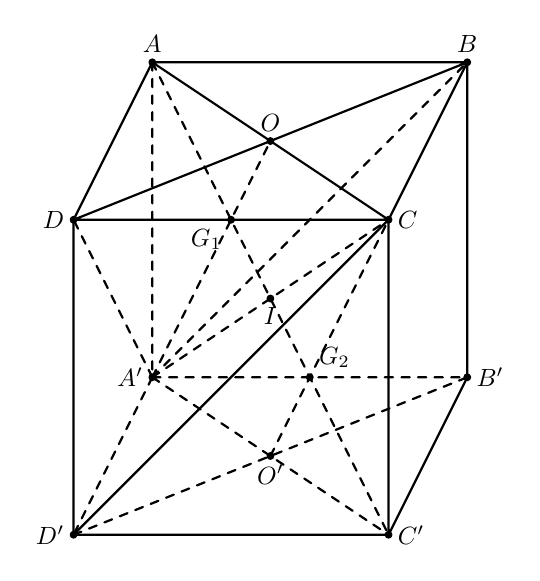
\begin{tikzpicture}[line join=round,line cap=round,>=stealth,thick]
     \coordinate (A) at (-2,2); 
     \coordinate (B)  at (2,2);
     \coordinate  (C) at (1,0);
     \coordinate  (D) at (-3,0);
     \coordinate (A') at  (-2,-2);
     \coordinate (B') at (2,-2); 
     \coordinate (C') at  (1,-4);
     \coordinate  (D') at (-3,-4);
     \coordinate (O) at (intersection of A--C and  B--D);
     \coordinate (O') at (intersection of A'--C' and B'--D'); 
      \coordinate (I) at (intersection of A--C' and A'--C);
     \coordinate (G_1) at (intersection of A--C' and  A'--O);
     \coordinate  (G_2) at (intersection of A--C' and O'--C);
     \draw[dashed] (A)--(A') 
      (A')--(B') 
      (A')--(D') 
       (A')--(B)
      (A')--(D) 
       (D')--(B')
      (O')--(C) 
       (A')--(C)
      (A')--(O) 
       (A)--(C')
      (A')--(C'); 
     \draw  (A)--(B)
       (A)--(D)
      (D)--(C) 
       (C)--(B)
       (A)--(C)
       (D)--(B)
       (D)--(D')
       (C)--(C')
       (B)--(B')
       (D')--(C)
      (D')--(C') 
       (C')--(B');
     \foreach \i in {A,B}{\draw (\i)  node[scale=0.9,above]{$\i$};}
      \foreach \i in {D,D',A'}{\draw (\i) node[scale=0.9,left]{$\i$};}
     \foreach \i in {C,C',B'}{\draw (\i)  node[scale=0.9,right]{$\i$};}
     \foreach \i in {O',I}{\draw (\i) node[scale=0.9,below]{$\i$};} 
     \foreach \i in {O}{\draw (\i)  node[scale=0.9,above]{$\i$};}
     \foreach \i in {G_2}{\draw (\i)  node[scale=0.9,above right]{$\i$};}
     \foreach \i in  {G_1}{\draw (\i) node[scale=0.9,below left]{$\i$};}
     \foreach \i in {A,B,C,D,A',B',C',D',G_1,G_2,O',O,I}{\draw[fill=](\i) circle  (1pt);}
    \end{tikzpicture}
  \end{center}
  \begin{itemchoice}
   \itemch \textbf{Đúng}. Vì $ABCD.A'B'C'D'$  là hình hộp nên\\ $\heva{& A'D' \parallel BC\\& A'D'=BC} \Rightarrow A'D'CB$ là hình bình hành.\\
    Suy ra $AB \parallel CD \Rightarrow AB \parallel(BDC).\quad(1)$
   \itemch \textbf{Đúng}. Ta  có $\heva{&A'B' \parallel CD \\& A'B'=CD} \Rightarrow A'B'CD$ là hình bình hành.\\
   Suy ra $A'D \parallel B'C  \Rightarrow A'D \parallel (B'D'C).\quad(2)$\\
   Từ $(1)$ và $(2)$  suy ra $(A'BD) \parallel(B'D'C)$.
   \itemch \textbf{Đúng}. Gọi $O$,  $O'$, $I$ theo thứ tự là tâm của các hình bình hành $ABCD$, $A'B'C'D'$, $ACC'A'$.\\
   Vì $G_1$ là trọng tâm tam giác $AB'D$  nên $\dfrac{A'G_1}{A'O}=\dfrac{2}{3}$.\\ $\Rightarrow G_1$ là trọng tâm tam giác $A'AC$, suy ra $G_1=AI \cap A'O. \quad(3)$\\
   Tương tự, $G_2$ là trọng tâm tam giác $B'D'C$ nên $\dfrac{CG_2}{CO'}=\dfrac{2}{3}$.\\ $\Rightarrow G_2$ là trọng tâm tam  giác $A'C'C$, suy ra $G_2=C'I \cap CO'.\quad(4)$. \\
   Từ $(3)$ và  $(4)$ suy ra $G_1$, $G_2$ cùng thuộc $AC'$.
   \itemch \textbf{Sai}. 
   Ta có $\dfrac{A G_1}{A I}=\dfrac{2}{3} \Rightarrow \dfrac{A G_1}{A C'}=\dfrac{1}{3}$; $\dfrac{C'G_2}{C'I}=\dfrac{2}{3}  \Rightarrow \dfrac{C'G_2}{A C'}=\dfrac{1}{3}$.\\
   Do  vậy $AG_1=G_1G_2=G_2C'=\dfrac{1}{3} AC'$.\\
   Vậy $G_1$, $G_2$ cùng thuộc $AC'$,  đồng thời chia $AC'$ thành ba phần bằng nhau.
 \end{itemchoice} }
\end{ex}

% nguồn: Ok_dungsai_lop11_Lan1
\begin{ex}%[1H4H3-3]%[ma:a7f56c5c]
 Cho tứ diện $ABCD$, gọi $I$ và $J$ lần lượt là trung điểm của $AD$ và $AC$, $G$ là  trọng tâm của tam giác $BCD$.
  \choiceTF
  {\True $IJ \parallel  CD$}
  {Giao tuyến của hai mặt phẳng $(GIJ)$ và $(BCD)$ là đường thẳng  qua $G$ và song song với $BC$}
  {Cho biết $CD=6$.  Biết $(GIJ)$ cắt $BC$, $BD$ lần lượt tại $M$ và $N$. Khi đó\break $2IJ+3MN=17$}
  {\True Cho biết $CD=6$. Biết $(GIJ)$ cắt $BC$, $BD$  lần lượt tại $M$ và $N$. Khi đó\break $3IJ+2MN=18$}
 \loigiai{\begin{center}
  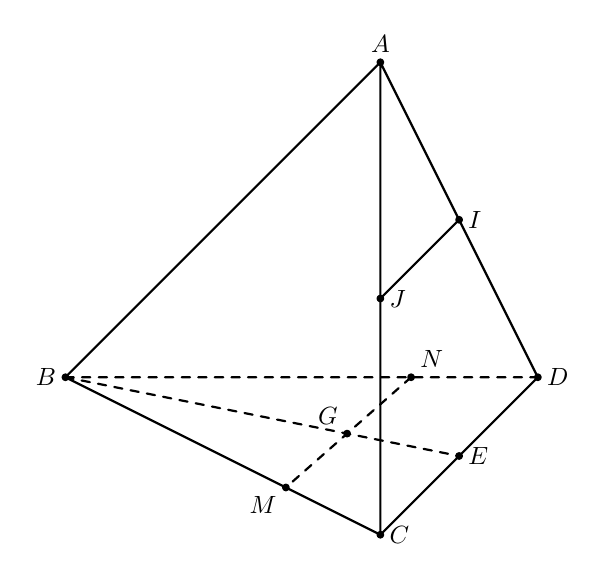
\begin{tikzpicture}[line join=round,line cap=round,>=stealth,thick]
    \coordinate (A)  at (0,4);
     \coordinate (B) at (-4,0);
    \coordinate  (C) at (0,-2);
    \coordinate  (D) at (2,0);
    \coordinate (E) at (1,-1); 
    \coordinate (N) at (0.39,0); 
    \coordinate  (M) at (-1.2,-1.4);
    \coordinate (J) at (0,1); 
     \coordinate (I) at (1,2);
     \coordinate (G) at (intersection of B--E and M--N);
    \draw (A)--(B) 
      (B)--(C)
      (C)--(D)
     (D)--(A) 
     (A)--(C) 
     (J)--(I); 
    \foreach \i in {A,B,C,D,G,M,N,E,J,I}{\draw[fill=](\i)  circle (1pt);}
     \draw[dashed](B)--(E)
      (B)--(D)
     (N)--(M); 
     \foreach \i in {A}{\draw (\i) node[scale=0.9,above]{$\i$};}
    \foreach \i in  {B}{\draw (\i) node[scale=0.9,left]{$\i$};}
    \foreach \i in {D,C,E,J,I}{\draw (\i)  node[scale=0.9,right]{$\i$};}
    \foreach \i in {G}{\draw (\i) node[scale=0.9,above left]{$\i$};} 
    \foreach \i in {M}{\draw (\i) node[scale=0.9,below  left]{$\i$};}
    \foreach \i in {N}{\draw (\i) node[scale=0.9,above right]{$\i$};} 
   \end{tikzpicture}
 \end{center}
 \begin{itemchoice}
  \itemch \textbf{Đúng}. Xét $\triangle ACD$ có $I$, $J$ lần lượt là trung điểm $AD$ và $AC$.\\ Suy ra $IJ$ là đường trung  bình tam giác $ACD$.
  Vậy $IJ\parallel  CD$
   \itemch \textbf{sai}.
  Vì $IJ$ là  đường trung bình của tam giác $ACD$ nên $IJ \parallel CD$.\\
  Ta có $\heva{&G\in(GIJ) \cap(BCD) \\& IJ \parallel  CD \\ &IJ \subset(GIJ),\, CD \subset(BCD)} \Rightarrow Gx=(GIJ) \cap(BCD)$.\\
  Suy ra $Gx$ là đường thẳng qua  $G$
  và  $Gx \parallel IJ \parallel CD$.
  \itemch \textbf{sai}. Trong mặt phẳng $(BCD)$, kẻ $Gx$ song song $CD$ cắt $BC$  tại $M$, cắt $BD$ tại $N$.\\
  Gọi $E$ là trung  điểm $CD$, theo định lí Thalès.\\
  Ta  có
   $\dfrac{BM}{BC}=\dfrac{BG}{BE}=\dfrac{2}{3}$ (vì $GM \parallel CE$), $\dfrac{MN}{CD}=\dfrac{BM}{BC}$ (vì $MN \parallel CD$).\\
  Suy ra $\dfrac{MN}{CD}=\dfrac{2}{3}$ hay $MN=\dfrac{2}{3} CD=\dfrac{2}{3} \cdot  6=4$.\\
  Vì $IJ$ là đường trung bình tam giác $ACD$ nên $IJ=\dfrac{1}{2}  CD=\dfrac{1}{2} \cdot 6=3$.\\
  Do  đó $2IJ+3MN=2\cdot 3+3 \cdot 4=18$.
  \itemch \textbf{Đúng}. $3IJ+2MN=3 \cdot 3+2 \cdot 4=17.$ 
 \end{itemchoice}
} 
\end{ex}

% nguồn: Ok_dungsai_lop11_Lan1
\begin{ex}%[1H4H3-3]%[ma:62193464]
 Cho hình  chóp $S.A B C D$, biết $A B$ cắt $C D$ tại $E, A C$ cắt $B D$ tại $F$ trong mặt phẳng đáy. Các khẳng định sau \textbf{đúng} hay \textbf{sai}?
 \choiceTF 
  {\True Đường thẳng $E F$ nằm trong  mặt phẳng $(A B C D)$}
  {\True $A B$ là giao tuyến của hai mặt  phẳng $(S A B)$ và $(A B C D)$}
  {$S F$ là giao tuyến của hai mặt phẳng  $(S A B)$ và $(S C D)$}
  {$S E$ là giao tuyến của hai mặt  phẳng $(S A C)$ và $(S B D)$}
 \loigiai{ 
  \begin{center}
   \begin{tikzpicture}[>=stealth,line join=round,line cap=round,font=\footnotesize,scale=0.8]
     \path 
      (0,0) coordinate (A) 
      (1,-2)  coordinate (D)
      (8,0)  coordinate (E)
      ($(E)!0.6!(A)$) coordinate  (B)
      ($(E)!0.7!(D)$) coordinate  (C)
      ($(A)+(1.5,4)$) coordinate  (S)
      (intersection of A--C and B--D)  coordinate (F);
     \draw  (S)--(A)--(D)--(S)--(C)--(D)
       (S)--(E)--(C);
      \draw[dashed](S)--(F)--(E)--(A)--(C)--(B)--(D)
      (S)--(B);; 
      \foreach \x/\y in {A/180,B/30,C/-40,D/180,F/190,E/0,S/90}
     \draw[fill=black] (\x) circle  (1.1pt) + (\y:0.5cm) node {$\x$};
    \end{tikzpicture}
  \end{center}
  \begin{itemchoice}
   \itemch Đúng. Ta có $E=A  B \cap C D \Rightarrow E \in A B, A B \subset(A B C D) \Rightarrow E \in(A B C D)$.\\
   Tương tự: $F=A  C \cap B D \Rightarrow F \in A C, A C \subset(A B C D) \Rightarrow F \in(A B C D)$. \\
   Vậy $E  F \subset(A B C D)$.
   \itemch Đúng. Vì $A$ là điểm chung của hai mặt phẳng $(S A B)$ và $(A B C D), B$ cũng là điểm chung của hai mặt phẳng $(S A B)$ và $(A B C  D)$.
   \itemch  Sai. Vì $S$ là điểm chung của hai mặt phẳng $(S A B)$ và $(S C D)$.\\
   Ta có $\heva{& E \in A B, A B \subset(S A B) \\ & E \in C D, C D \subset(S C D)}$ $\Rightarrow  E \in(S A B) \cap(S C D)$.\\
   Vậy  $S E=(S A B) \cap(S C D)$.
   \itemch Sai. Vì $S$ là điểm  chung của hai mặt phẳng $(S A C)$ và $(S B D)$.\\
   Ta có $\heva{ &F \in  A C, A C \subset(S A C) \\ & F \in B D, B D \subset(S B D)}$ $\Rightarrow F \in(S A C) \cap(S B D)$.\\
   Vậy $S F=(S A C) \cap(S B D)$. 
  \end{itemchoice}
 } 
\end{ex}

% nguồn: Ok_dungsai_lop11_Lan1
\begin{ex}%[1H4H3-3]%[ma:7ea50bff]
 Cho hình chóp $S.ABCD$ có đáy $ABCD$ là hình bình hành. Lấy điểm $M$ trên cạnh $AD$ sao  cho $AD=3AM$. Gọi $G$, $N$ theo thứ tự là trọng tâm các tam giác $SAB$, $ABC$. Khi đó
  \choiceTF
   {Giao tuyến của hai mặt phẳng $(SAB)$ và $(SCD)$ là đường thẳng đi qua $S$ và song song với $AC$, $BD$}
   {$\dfrac{DN}{DB}=\dfrac{1}{3}$}
  {\True $MN$ song song  với mặt phẳng $(SCD)$}
  {$NG$ cắt với  mặt phẳng $(SAC)$}
 \loigiai{\begin{center}
  \begin{tikzpicture}[>=stealth,line join=round,line cap=round]
    \draw[dashed]  (0,0) coordinate (A)--(-130:3) coordinate (B)
     (5,0) coordinate (D)--(A)--($(A)+(80:4)$) coordinate (S) 
     ($(B)+(D)-(A)$)  coordinate (C);
    \coordinate (O)  at ($(A)!0.5!(C)$);
    \coordinate (M) at ($(A)!1/4!(D)$); 
    \coordinate (x) at ($(S)+(B)-(A)$); 
    \coordinate  (P) at ($(A)!1/2!(B)$);
    \coordinate  (G) at ($(S)!2/3!(P)$);
     \coordinate (y) at ($(S)!-2/3!(x)$);
     \path (intersection of P--C and B--O) coordinate (N);
    \draw[black,scale=2.5] (B)--($(D)-(A)+(B)$) coordinate (C)--(D)--(S)--(B) 
      (S)--(C)
      (y)--(S)--(x);
    \draw[dashed](A)--(C) 
     (B)--(D) 
      (S)--(P)--(C)
     (M)--(N)--(G); 
    \foreach \diem/\vitrin in {S/above,A/above right,B/below left,C/below  right,D/right,O/below,M/above right,P/left, N/below,G/right,x/left} \fill (\diem) circle (1pt) node[\vitrin]{$\diem$};
   \end{tikzpicture}
 \end{center}
 \begin{itemchoice}
   \itemch \textbf{Sai}.\\
  Ta có $\heva{&S\in (SAB)\cap (SCD)\\&AB\parallel  CD\\&AB\subset (SAB),CD\subset (SCD)}\Rightarrow (SAB)\cap (SCD)=Sx$.\\ (với $Sx$ qua $S$ và $Sx\parallel AB\parallel CD$).
   \itemch \textbf{Sai}.\\
  Gọi $O$ là tâm hình  bình hành $ABCD$.
   Vì $N$ là trọng tâm của $\triangle ABC$ nên $BN=\dfrac{2}{3}BO=\dfrac{2}{3} \cdot \dfrac{1}{2} BD=\dfrac{1}{3} BD\Rightarrow \dfrac{DN}{DB}=\dfrac{2}{3}$.
  \itemch \textbf{Đúng}.\\ 
  Ta có $AD=3AM\Rightarrow  \dfrac{DM}{DA}=\dfrac{2}{3}$.\\
   Xét tam giác $ADB$, ta có $\dfrac{DM}{DA}=\dfrac{DN}{DB}=\dfrac{2}{3}$ nên\\ $MN\parallel AB\Rightarrow MN\parallel CD$,
  mà $CD\subset (SCD)\Rightarrow MN\parallel  (SCD)$.
  \itemch  \textbf{Sai}.\\
  Gọi $P$ là trung điểm $AB$. Tam giác $SPC$  có
  $\dfrac{PG}{PS}=\dfrac{PN}{PC}=\dfrac{1}{3}$ (tính chất  trọng tâm)
  \[\Rightarrow NG\parallel SC,\,SC\subset  (SAC)\Rightarrow NG\parallel (SAC).\]
 \end{itemchoice}
 }
\end{ex}

% nguồn: Ok_dungsai_lop11_Lan1
\begin{ex}%[1H4H3-3]%[ma:7d914cab]
 Cho hình chóp $S.ABC$. Gọi $I$, $J$ lần lượt là trung điểm của $AB$ và $BC$. Gọi $H$, $K$ lần lượt là trọng tâm của $\triangle SAB$ và $\triangle  SBC$. Khi đó
 \choiceTF 
  {\True  $AC\parallel (SIJ)$}
   {$HK$ cắt $IJ$}
   {\True $HK\parallel (SAC)$}
  {\True Giao tuyến của $(BHK)$ và $(ABC)$ là đường thẳng  đi qua $B$ và song song với $AC$}
 \loigiai{ 
  \begin{center}
   \begin{tikzpicture}[>=stealth,line join=round,line cap=round,scale=1.5,font=\footnotesize]
     \draw[black,scale=2.5] (0,0)  coordinate (A)--(-35:0.8) coordinate (B)--(1,0) coordinate (C)--($(A)+(70:1)$) coordinate (S)--(B)
      (S)--(A); 
     \coordinate (I) at  ($(A)!0.5!(B)$);
     \coordinate (J) at ($(C)!0.5!(B)$); 
     \coordinate (M)  at ($(S)!0.5!(B)$);
     \path (intersection of A--M  and S--I) coordinate (H);
     \path (intersection of  M--C and S--J) coordinate (K);
     \draw[dashed,black,scale=2.5] (A)--(C) 
       (I)--(J)
      (H)--(K); 
      \draw (S)--(I)
       (S)--(J)
       (A)--(M)--(C);
     \foreach \diem/\vitrin in {S/above,A/left,B/below left,C/right,I/below,J/right,H/left,K/right}  \fill (\diem) circle (.75pt) node[\vitrin]{$\diem$};
    \end{tikzpicture}
  \end{center}
  \begin{itemchoice}
    \itemch \textbf{Đúng}. Vì $IJ$ là đường trung bình $\triangle ABC$ nên $IJ\parallel AC$.\\
   Ta có $\heva{&AC\parallel  IJ\\&IJ\subset (SIJ)\\&AC\not \subset (SIJ)} \Rightarrow AC\parallel (SIJ)$.
   \itemch \textbf{Sai}. Ta có $\dfrac{SH}{HI}=\dfrac{SK}{KJ}=2$ ($H$, $K$ lần lượt là trọng tâm $\triangle SAB$ và $\triangle SAC)$. 
   $\Rightarrow HK\parallel IJ$. 
   \itemch \textbf{Đúng}. Ta có $\heva{&HK\parallel AC \,(HK\parallel IJ,\,AC\parallel IJ)\\&AC\subset (SAC)\\&HK\not \subset (SAC)} \Rightarrow HK\parallel  (SAC)$.
   \itemch \textbf{Đúng}. Ta có $\heva{&HK\parallel AC\\&HK\subset (BHK)\\&AC\subset (ABC)\\&B\in (BHK)\cap (ABC)}$.\\ 
   Vậy giao tuyến của $(BHK)$ và $(ABC)$ là đường thẳng $Bx$ đi qua $B$ và song song với $AC$ và  $HK$.
 \end{itemchoice}   }
\end{ex}

% nguồn: Ok_dungsai_lop11_Lan1
\begin{ex}%[1H4H3-3]%[ma:d7f40e6b]
 Cho hình chóp $S.ABCD$ với $ABCD$ là hình bình hành tâm $O$. Gọi $M$, $N$, $P$ lần lượt là trung điểm các cạnh $SA$,  $BC$, $CD$.
  \choiceTF
  {Giao tuyến của mặt phẳng $\left(SAB\right)$ với mặt phẳng $\left(SCD\right)$ là đường thẳng đi qua $S$ và song song  với $AD$}
  {\True Giao tuyến của mặt  phẳng $\left(MNP\right)$ với mặt phẳng $\left(MBD\right)$ là đường thẳng đi qua $M$ và song song với $BD$}
  {\True Giao tuyến của mặt phẳng $\left(MOP\right)$ với mặt phẳng $\left(SAD\right)$ là đường thẳng đi qua $M$ và song song với  $AD$}
  {\True Mặt phẳng $\left(\alpha\right)$ đi qua $N$ và song song với $SA$ và $CD$. Giao tuyến của $\left(\alpha\right)$  với $\left(SAC\right)$ là đường thẳng đi qua $O$ và song song với $SA$}
  \loigiai{
  \begin{center}
   \begin{tikzpicture}[scale=0.7,font=\footnotesize,line join=round,line cap=round,>=stealth,extended line/.style={shorten >=-#1,shorten <=-#1},
    extended line/.default=1cm]
    \path
     (0,0) coordinate (A)
    (-3,-3)  coordinate (D)
    (4,-3)  coordinate (C)
    ($(A)+(C)-(D)$) coordinate (B) 
    (2,6) coordinate (S) 
    ($(S)!0.5!(A)$) coordinate  (M)
    ($(B)!0.5!(C)$) coordinate  (N)
    ($(C)!0.5!(D)$) coordinate  (P)
    (intersection of A--C and  D--B) coordinate (O)
    ($(S)!1/2!(C)$) coordinate  (T);
    \draw (S)--(B)--(C)--(S)--(D)--(C);
   \draw[dashed] (S)--(A)--(D) 
     (A)--(B)
    (M)--(N)--(P)--cycle (A)--(C) 
    (B)--(D)--(M)--cycle  (M)--(O)--(P)
     (O)--(T);
   \draw [extended line=0.5cm] (S) -- +($(B)-(A)$) node[above]{$ x $};
   \draw [extended line=0.5cm,dashed] (M) -- +($(B)-(O)$) node[above]{$ y $};
   \draw [extended line=0.5cm,dashed] (M) -- +($(P)-(O)$) node[above]{$ z $};
   \foreach \p/\q  in {S/90,A/-90,B/-90,C/-90,D/-90,M/150,P/-90,T/0,N/0,O/-90}
   \fill[black] (\p) circle (1.0pt) node[shift={(\q:3.5mm)}]{$\p$}; 
   \end{tikzpicture}
  \end{center}
  \begin{itemchoice}
   \itemch \textbf{Sai}.  Ta có
   $\heva{&S\in\left(SAB\right)\cap\left(SCD\right)\\& 
   AB\parallel CD  \\&
   AB  \subset\left(SAB\right),\, CD \subset\left(SCD\right)}
   \Rightarrow\left(SAB\right)\cap\left(SCD\right)=Sx\parallel  AB \parallel CD$.
   \itemch \textbf{Đúng}.  Ta có
   $\heva{&M\in\left(MNP\right)\cap\left(MBD\right)\\ 
   &NP\parallel BD\\ 
    &NP\subset\left(MNP\right)\\
    &BD \subset\left(MBD\right)}\Rightarrow\left(MNP\right)\cap\left(MBD\right)=My\parallel NP\parallel BD$.
    \itemch \textbf{Đúng}. Ta có
   $\heva{ 
    &M\in\left(MOP\right)\cap\left(SAD\right)\\
   &OP\parallel  AD\\
   &OP \subset\left(MOP\right),\, AD  \subset\left(SAD\right).}$\\
   $\Rightarrow\left(MOP\right)\cap\left(SAD\right)=Mz\parallel OP  \parallel AD$.
   \itemch  \textbf{Đúng}. Ta có
    $\heva{&N\in\left(\alpha\right)\cap\left(ABCD\right)\\
   &CD\parallel \left(\alpha\right)\\ 
    &CD\subset\left(ABCD\right)}
   \Rightarrow\left(\alpha\right)\cap\left(ABCD\right)=NK\,  \left(NK \parallel CD,\, K\in AD\right)$.\\
   Ta  có $NK$ đi qua $O$ ($NK\parallel CD$ và $N$ là trung điểm của $BC$).\\
    $\heva{&O\in\left(\alpha\right)\cap\left(SAC\right)\\&
   SA  \parallel \left(\alpha\right)\\
   &SA\subset\left(SAC\right) }\Rightarrow\left(\alpha\right)\cap\left(SAC\right)=OT\, \left(OT\parallel SA,\, T\in  SC\right)$.
 \end{itemchoice}}
\end{ex}

% nguồn: Ok_dungsai_lop11_Lan2
\begin{ex}%[1H4H3-3]%[ma:89d0caa2]
	Cho hình chóp $S. ABCD$ có đáy $ABCD$ là hình thang và $AB\parallel CD$. Gọi $M$ là trung điểm của $SD$ và $(P)$  là mặt phẳng qua $M$ và song song với $(SAB)$. Xét tính đúng sai của các khẳng định sau
	\choiceTF 
		{Mặt  phẳng $(P)$ song song với mặt phẳng $(SCD)$}
		{\True Đường  thẳng $AB$ song song với mặt phẳng $(P)$}
		{\True Đường thẳng $CD$ cũng song song với mặt phẳng $(P)$} 
		{\True Giao điểm của $(P)$ và $SC$ là điểm $N$ với $N$ là trung  điểm của $SC$}
	 \loigiai{
		\begin{center}
			\begin{tikzpicture}[line join = round,line cap = round,>=stealth,font=\footnotesize,scale=1,declare function={ad=2; cd=2; ab=4.5; gs=80; sa=3; gocA=-50;}]
					\path 
						(0,0) coordinate  (A)
						(ab,0) coordinate  (B)
						(gocA:ad) coordinate  (D)
						($(D)+(cd,0)$) coordinate (C) 
						(gs:sa) coordinate (S) 
						($(S)!0.5!(C)$) coordinate  (N)
						($(S)!0.5!(D)$)  coordinate (M)
						($(A)!0.5!(D)$)  coordinate (tad)
						($(C)!0.5!(B)$) coordinate (tcb); 
					 \draw (S)--(A)--(D)--(C)--(B)--(S)--(C)
						 (S)--(D)
						 (tad)--(M)--(N)--(tcb);
					\draw[dashed] (B)--(A) 
						(tcb)--(tad); 
					\foreach \x/\gm in {A/180,B/0,C/-90,D/-90,S/90,M/150,N/30} \fill (\x)  circle (1pt)
						($(\x)+(\gm:3.5mm)$)  node{$\x$};
				\end{tikzpicture}
		\end{center}
		\begin{itemchoice}
			\itemch Mặt phẳng $(P)$ cắt mặt phẳng  $(SCD)$.
			\itemch Hai mặt phẳng $(P)$ và $(SCD)$ có điểm  $M$ chung. Giả sử $(P)$ cắt $SC$ tại điểm $N$.
			Khi đó $MN=(P) \cap(SCD)$  mà $(P) \parallel(SAB)$ nên $AB\parallel(P)$.
			 \itemch Lại có $CD\parallel AB, CD\not \subset(P)$ nên $CD\parallel(P)$.
			\itemch Từ đó suy ra $MN\parallel CD$, mà $M$ là trung điểm  của $SD$ nên $N$ là trung điểm của $SC$.
		\end{itemchoice}
	} 
\end{ex}

% nguồn: Ok_dungsai_lop11_Lan2
\begin{ex}%[1H4H3-3]%[ma:6b0e93dd]
	Cho hình chóp $S.ABCD$ đáy $ABCD$ là hình bình hành tâm $H$. Mặt phẳng $(P)$ đi  qua $H$ và song song với $(SAB)$.
	\choiceTF 
		{\True Giao tuyến của mặt phẳng $(P)$ và mặt phẳng $(ABCD)$ là $EF$ với $E, F$ lần lượt là trung điểm của  $BC$ và $AD$}
		 {Giao tuyến của mặt phẳng $(P)$ và mặt phẳng $(SBC)$ là $EK$ với $K$ là trung điểm của $SD$}
		{Giao tuyến của mặt phẳng $(P)$ và mặt phẳng $(SAD)$  là $FI$ với $I$ là trung điểm của $FE$}
		{\True Giao tuyến của mặt phẳng  $(P)$ và mặt phẳng $(SBC)$ là đường thẳng $KE$}
	\loigiai{ 
		\begin{itemchoice}
			\itemch Ta có  $H$ là một điểm chung của mặt phẳng $(P)$ và mặt phẳng $(ABCD),(P) \parallel(SAB)$ $(ABCD. \cap(SAB)=AB$ nên giao tuyến của $(P)$ và $(ABCD)$ là đường thẳng qua $H$, song song với $AB$, cắt $BC$ và $AD$ lần lượt tại $E, F$.\\
			Do $H$ là tâm hình bình  hành $ABCD$ nên $E, F$ là trung điểm của $BC$ và $AD$.
			\itemch Theo cách dựng  trên ta có $(P)$ và $(SBC)$ có điểm chung $E$.\\
			 Mặt phẳng $(P) \parallel(SAB),(SBC) \cap(SAB)=SB$ nên giao tuyến của $(P)$ và $(SBC)$ là đường thẳng qua $E$, song song với $SB$, cắt $SC$ tại $K$.\\
			Khi đó $EK$ là đường  trung bình của tam giác $SBC$ nên $K$ là trung điểm của $SC$.
			\begin{center}
				\begin{tikzpicture}[line join = round,line cap = round,>=stealth,font=\footnotesize,scale=1,declare function={ab=2.5; ad=4.5; gs=110; sa=3; gocA=-130;}]
						 \path
						(0,0)  coordinate (A)
						(ad,0)  coordinate (D)
						(gocA:ab) coordinate  (B)
						($(D)-(A)+(B)$) coordinate (C) 
						(gs:sa) coordinate (S) 
						($(A)!0.5!(D)$) coordinate (F) 
						($(B)!0.5!(C)$) coordinate  (E)
						($(S)!0.5!(C)$)  coordinate (K)
						 ($(S)!0.5!(D)$) coordinate (I)
						(intersection of  A--C and B--D) coordinate (H);
						\draw  (S)--(B)--(C)--(D)--(S)--(C)
						(E)--(K)--(I); 
						\draw[dashed]  (S)--(A)--(D)
						(B)--(A) 
						(E)--(F)--(I) 
						(A)--(C) 
						(B)--(D); 
						\foreach \x/\gm in {A/150,B/180,C/-20,D/0,S/90,H/-70,I/90,K/180,E/-90,F/70}  \fill (\x) circle (1pt)
						 ($(\x)+(\gm:3.5mm)$) node{$\x$};
					\end{tikzpicture}
			\end{center}
			\itemch Tương tự ta có giao tuyến của $(P)$  và $(SAD)$ là đường thẳng qua $F$, song song với $SA$ và cắt $SD$ tại $I$. Khi đó $I$ là trung điểm của $SD$.
			\itemch Từ các kết  quả trên ta có $(P) \cap(ABCD)=EF,(P) \cap(SAD)=FI,(P) \cap(SCD)=IK$ $(P) \cap(SBC)=KE$.
		\end{itemchoice}
	 }
\end{ex}

% nguồn: Ok_dungsai_lop11_Lan2
\begin{ex}%[1H4H3-3]%[ma:4298f3eb]
	 Cho tứ diện $ABCD$. Giả sử $M$ thuộc đoạn thẳng $BC$. Mặt phẳng $(\alpha)$ qua $M$ song song với $AB$ và $CD$. Khi đó
	\choiceTF 
		{\True Giao tuyến của mặt  phẳng $(\alpha)$ với mặt phẳng $(ABC)$ là đường thẳng đi qua $M$ và song song với $AB$}
		{\True Giao  tuyến của mặt phẳng $(\alpha)$ với mặt phẳng $(BCD)$ là đường thẳng đi qua $M$ và song song với $CD$}
		{\True Giao  tuyến của mặt phẳng $(\alpha)$ với mặt phẳng $(ABD)$ là đường thẳng đi qua $N$ và song song với $AB$}
		{Hình tạo bởi các giao tuyến của mặt phẳng $(\alpha)$ với các mặt của tứ diện (ta gọi là thiết diện) là  hình thang}
	 \loigiai{
		\begin{center}
			\begin{tikzpicture}[scale=1,font=\footnotesize,line join=round,line cap=round,>=stealth]
					\def\canhBD{4}; \def\canhCB{2}; \def\gocCBD{-50};  \def\h{3};
					 \coordinate (B) at (0,0);
					\coordinate  (C) at ($(B)+(\gocCBD:\canhCB)$);
					 \coordinate (D) at ($(B)+(0:\canhBD)$);
					\coordinate  (O) at ($ 1/3*(B)+1/3*(C)+1/3*(D)$);
					\coordinate  (A) at ($(O)+(90:\h)$);
					 \path
						($(B)!1/3!(C)$)  coordinate (M)
						($(B)!1/3!(D)$) coordinate  (N)
						($(A)!1/3!(C)$) coordinate  (Q)
						 ($(A)!1/3!(D)$) coordinate (P);
					\draw (A)--(C) 
						 (A)--(B)--(C)
						(A)--(D)--(C) 
						 (M)--(Q)--(P);
					\draw[dashed]  (B)--(D)
						 (M)--(N)--(P);
					\foreach \x/\y in {A/90,B/180,C/-90,D/0,M/-150,N/120,P/60,Q/150}{\fill (\x)  circle (1pt)
						($(\x)+(\y:0.3cm)$) node{$\x$};} 
				\end{tikzpicture}
		\end{center}
		\begin{itemchoice}
			\itemch {\bf Đúng}.\\ 
			Vì $(\alpha)\parallel AB$ nên giao tuyến của mặt phẳng $(\alpha)$ với mặt phẳng $(ABC)$ là đường thẳng đi qua $M$ và song song với $AB$ và cắt  $AC$ tại $Q$.
			\itemch  {\bf Đúng}.\\
			Vì $(\alpha)\parallel CD$ nên giao tuyến của mặt phẳng $(\alpha)$ với mặt  phẳng $(BCD)$ là đường thẳng đi qua $M$ và song song với $CD$ và cắt $BD$ tại $N$.
			\itemch {\bf  Đúng}.\\
			Vì $(\alpha) $ nên giao tuyến của mặt phẳng $(\alpha)$ với mặt phẳng $(ABD)$ là đường thẳng đi qua $N$  và song song với $AB$ và cắt $AD$ tại $P$.
			\itemch  {\bf Sai}.\\
			Ta có $MN\parallel PQ \parallel  CD$, $MQ\parallel PN\parallel AB$.\\
			Vậy hình tạo bởi các giao tuyến của mặt phẳng $(\alpha)$ với  các mặt của tứ diện (ta gọi là thiết diện) là hình bình hành $MNPQ$.
		\end{itemchoice}
	} 
\end{ex}

% nguồn: Ok_dungsai_lop11_Lan2
\begin{ex}%[1H4H3-3]%[ma:62691521]
	Cho hình chóp $S.ABCD$ có đáy là hình bình hành tâm $O$. Gọi $M$, $N$ lần lượt là trung điểm  của $SB$ và $SC$, lấy điểm $P\in SA$.
	 \choiceTF
		{Giao tuyến $(SAB)$ và $(SCD)$ là  đường thẳng $d$ đi qua $S$ và song song với $AC$ và $BD$}
		{Giao điểm $SD$ và $(MNP)$ là $R$ với $R=QN\cap  SD$}
		{Ba  đường thẳng $PR$; $MN$; $AD$ đôi một song song}
		{$OJ\parallel (SAD)$} 
	 \loigiai{
		\begin{center}
			\begin{tikzpicture}[line join = round,line cap = round,>=stealth,font=\footnotesize,scale=1,declare function={ad=2.5; ab=4.5; gs=80; sa=4.5; gocA=-130;}]
					 \path
						 (0,0) coordinate (A)
						 (ab,0) coordinate (B)
						(gocA:ad) coordinate (D) 
						($(B)-(A)+(D)$) coordinate (C) 
						(gs:sa) coordinate (S) 
						(intersection  of A--C and B--D) coordinate (O)
						($(S)!0.5!(B)$)  coordinate (M)
						 ($(S)!0.5!(C)$) coordinate (N)
						 ($(S)!0.35!(A)$) coordinate (P)
						(intersection of P--M and A--B)  coordinate (Q)
						(intersection of  P--N and S--O) coordinate (O')
						(intersection of  M--O' and S--D) coordinate (R)
						($(N)!0.5!(M)$) coordinate  (J)
						($(Q)-(A)+(S)$) coordinate (d); 
					\draw (S)--(D)--(C)--(B) 
						 (D)--(S)--(C)
						 (S)--(Q)
						 (B)--(Q)
						 (R)--(N)--(M);
					\draw[dashed]  (S)--(A)--(D)
						 (C)--(B)--(A)
						(S)--(B) 
						 (A)--(C)
						 (B)--(D)
						(R)--(P)--(Q) 
						 (P)--(N)
						 (O)--(J)
						(R)--(M) 
						(S)--(O); 
					\draw[shorten <= -1cm,shorten  >= 2cm] (S)--(d) node[above,pos=0.5]{$d$};
					\foreach \x/\gm in {A/150,B/-60,C/-20,D/180,S/90,P/30,M/30,R/180,N/-110,Q/0,O/-90,J/0,O'/-30}  \fill (\x) circle (1pt)
						($(\x)+(\gm:3.5mm)$)  node{$\x$};
				\end{tikzpicture}
		\end{center}
		\begin{itemchoice}
			\itemch Do $AB$ song song với $CD$ nên giao tuyến của $(SAB)$ và $(SCD)$  là đường thẳng $d$ đi qua $S$ và song song với $AB$ và $CD$.
			\itemch Ta có  $(SAC)\cap(SBD)=SO$.\\
			Trong $(SAC)$  Gọi $O'=SO\cap PN$.\\
			Trong  $(SBD)$ Gọi $R= MO'\cap SD$.\\
			Ta có $\heva{& R\in SD \\ &  R\in MO'\subset(PMN)}\Rightarrow SD\cap(PMN)=R$.
			\itemch Do $3$ mặt phẳng $(MNP)$; $(ABC)$; $(SAD)$ cắt nhau theo  $3$ giao tuyến là $PR$; $MN$; $AD$ nên chúng song song hoặc đồng quy.\\
			Mặt khác $MN \parallel AD\Rightarrow MN  \parallel AD \parallel PR$
			\itemch Ta có $OM$ là đường trung bình trong tam giác $SBD\Rightarrow OM\parallel  SD$.\\
			Tương tự  ta có $ON\parallel SA\Rightarrow(OMN) \parallel(SAD)$.\\
			Mặt khác $OJ\subset(OMN) \Rightarrow OJ\parallel(SAD)$. 
		\end{itemchoice}
	} 
\end{ex}

% nguồn: Ok_dungsai_lop11_Lan2
\begin{ex}%[1H4H3-3]%[ma:6e7af684]
	Cho lăng trụ tam giác  $ABC.A'B'C'$. Gọi $I$ và $I'$ lần lượt là trung điểm của $BC$ và $B'C'$.
	 \choiceTF
		{\True $II' \parallel  BB'$}
		{\True $AA'I'I$ là hình bình  hành}
		 {$IA'$ song song $(AB'C')$}
		 {\True Giao tuyến của $\left(AB'C'\right)$ và $\left(A'BC'\right)$ là đường thẳng đi qua giao điểm của hai đường thẳng $AI'$, $A'I$}
	 \loigiai{
		\begin{center}
			\begin{tikzpicture}[line join = round,line cap = round,>=stealth,font=\footnotesize,scale=.8,declare function={ab=3; ac=8; cao=4; gocA=-40;}]
					\path (0,0)  coordinate (A)
						(gocA:ab) coordinate (B) 
						(ac,0) coordinate (C) 
						($(A)+(90:cao)$)  coordinate (A')
						($(A')+(ac,0)$) coordinate (C') 
						 ($(A')+(gocA:ab)$) coordinate (B')
						($(B)!0.5!(C)$) coordinate (I) 
						($(B')!0.5!(C')$) coordinate  (I')
						(intersection  of A'--I and A--I') coordinate (E)
						 (intersection of A'--B and A--B') coordinate (F);
					\draw (A)--(B)--(C) 
						 (A')--(B')--(C')--cycle (A)--(A')
						 (B)--(B')
						(C)--(C') 
						(I)--(I') 
						 (A)--(B')
						 (A')--(B);
					\draw[dashed] (A)--(C) 
						(I)--(A)--(C') 
						 (A')--(I)
						(A)--(I'); 
					\foreach \x/\gm  in {A/180,B/-90,C/0,A'/90,C'/0,B'/70,I/-90,I'/90,F/180,E/90} \fill (\x) circle (1pt)
						($(\x)+(\gm:3.5mm)$) node{$\x$}; 
				\end{tikzpicture}
		\end{center}
		\begin{itemchoice}
			 \itemch Ta có $I'$, $I$ lần lượt là trung điểm của $B'C'$ và $BC$.\\
			Suy ra $II'$  là đường trung bình của hình bình hành $BB'C'C$.\\
			 Suy ra $II'=BB'$ và $II' \parallel BB'$.
			\itemch Ta có $\heva{& II'\parallel AA'\,\left(\parallel BB'\right)  \\ & II'=AA'\,\left(=BB'\right)}$\\
			$\Rightarrow AA'I'I$ là hình bình hành  $\Rightarrow AI\parallel A'I'$.
			\itemch Trong $(IAA'I')$ gọi $E=AI' \cap  A'I$\\
			$\Rightarrow\heva{& E\in AI';AI'\subset\left(AB'C'\right) \\ &  E\in A'I}\Rightarrow E=A'I\cap \left(AB'C'\right)$.
			\itemch Trong $(AA'B'B)$ gọi $F=AB' \cap A'B$ 
			$\Rightarrow\heva{&  F\in AB'; AB'\subset\left(AB'C'\right) \\ & F\in A'B;A'B\subset\left(A'BC'\right)}$\\
			$\Rightarrow F\in \left(AB'C'\right)\cap\left(A'BC'\right)\quad(1)$.\\ 
			Ta có $E=AI' \cap A' I\Rightarrow\heva{& E\in AI';AI'\subset\left(AB'C'\right)  \\ & E\in A'I;A'I\subset\left(A'BC'\right)}\Rightarrow E\in \left(AB'C'\right)\cap \left(A'BC'\right)\quad(2)$.\\
			Từ $(1)$ và $(2)$ suy ra  $EF=\left(AB'C'\right) \cap\left(A'BC'\right)$.
		\end{itemchoice}
	 }
\end{ex}

% nguồn: Ok_dungsai_lop11_Lan2
\begin{ex}%[1H4H3-3]%[ma:96a3c953]
	Cho hình lăng trụ tam giác $ABC.A'B'C'$. Gọi $E$, $F$ lần lượt là  trung diểm của các cạnh $AC$ và $A'B'$.
	 \choiceTF
		{\True Nếu gọi $M$  là trung điểm của $B'C'$ thì $FM=\dfrac{1}{2} A'C'$}
		{\True  $EF \parallel \left(BCC'B'\right)$}
		{Nếu gọi $K$ là trung điểm của $AB$ thì tứ giác $CC'FK$ là hình thang vuông} 
		{\True Gọi $I=CF\cap \left(AC'B\right)$ thì khi  đó $I$ là trung điểm đoạn thẳng $CF$}
	\loigiai{ 
		\begin{center}
			\begin{tikzpicture}[scale=2,font=\footnotesize,line join=round,line cap=round,>=stealth]
					\coordinate (A)  at (-2,0);
					 \coordinate (B) at (0,-1);
					 \coordinate (C) at (3,0);
					\coordinate (H)  at (1,4);
					\foreach \i in {A,B,C}{\coordinate (\i') at ($(\i)+(H)$);  \draw (\i)--(\i');}
					 \draw (A')--(B')--(C')--cycle;
					\draw (A)--(B)--(C); 
					\draw[dashed,thin](A)--(C); 
					 \coordinate (M) at ($(B')!0.5!(C')$);
					\coordinate  (F) at ($(B')!0.5!(A')$);
					\coordinate (K) at  ($(A)!0.5!(B)$);
					 \coordinate (E) at ($(A)!0.5!(C)$);
					\coordinate (I)  at ($(F)!0.5!(C)$);
					 \draw (C')--(F)--(M)--(C)
						(F)--(K); 
					 \draw[dashed,thin](A)--(C')--(K)--(C)--(F)--(E);
					\foreach \i/\g in {A/180,B/-90,C/0,A'/180,B'/-30,C'/0,M/90,F/180,K/-170,E/30,I/-90}{\draw[fill=black](\i) circle  (0.5pt)
						($(\i)+(\g:4mm)$) node[scale=1]{$\i$};} 
				\end{tikzpicture}
		\end{center}
		\begin{itemchoice}
			\itemch Gọi $M$ là trung điểm $B'C'$ ta có $FM$ là đường trung bình của $\Delta A'B'C'$ nên $FM$ song song và độ dài bằng nửa đoạn  $A'C'$.
			\itemch Lại có $E$ là trung điểm $AC$, $AC$ song  song và bằng $A'C'$ nên $EC$ song song và độ dài bằng nửa $A'C'$.\\
			Suy ra $FM$ song song và bằng $EC$,  nên $CEFM$ là hình bình hành.\\
			Do  đó $EF$ song song với $MC$ mà $MC$ nằm trong $\left(BCC'B'\right)$ nên $EF$ song song với $\left(BCC'B'\right)$.
			\itemch Gọi $K$ là trung điểm $AB$, vì $F$ là trung  điểm $A'B'$ và $ABB'A'$ là hình bình hành nên $FK$ song song và bằng $AA'$. Do đó $FK$ song song và bằng $CC'$, suy ra $CC'FK$ là hình bình hành.
			\itemch  Khi đó gọi $I$ là giao điểm của $CF$ và $KC'$ thì $I$ là trung điểm $CF$.\\
			Mặt khác $KC'\subset \left(AC'B\right)$ nên điểm $I$  xác định như trên chính là giao điểm của $CF$ và $\left(AC'B\right)$ theo yêu cầu đề bài.
		\end{itemchoice}
	 }
\end{ex}

% nguồn: Ok_dungsai_lop11_Lan1
\begin{ex}%[1H4V3-3]%[ma:f44bc5c0]
 Cho hình chóp $S.ABCD$ có đáy $ABCD$ là hình thang, $AB$ là đáy lớn, $O$ là giao điểm của $AC$ và $BD$. Gọi $M$, $N$  lần lượt là trung điểm của $SB$ và $SD$. Các mệnh đề sau đúng hay sai?
  \choiceTF
  {\True  $CD\parallel(SAB)$}
  {\True Giao tuyến của hai mặt phẳng $\left(CMN\right)$ và $\left(ABCD\right)$ là đường thẳng đi qua $C$ và  song song với $BD$}
  {Giao tuyến của hai mặt  phẳng $\left(SAD\right)$ và $\left(SBC\right)$ là đường thẳng đi qua $S$ và song song với $AD$, $BC$}
  {Gọi $P$ là trung điểm của $SC$, $I$ là giao điểm của $OP$ và $\left(CMN\right)$. Khi  đó $\dfrac{IP}{IO}=\dfrac{1}{4}$}
 \loigiai{ 
  \begin{center}
   \begin{tikzpicture}[line join = round,line cap = round,font=\footnotesize,>=stealth,scale=1]
     \coordinate (A) at  (-3,2);
     \coordinate (B) at (5,2); 
     \coordinate (D) at (0,0); 
     \coordinate (C) at  (3,0);
     \coordinate (S) at (1.5,5); 
      \coordinate (M) at ($(S)!0.5!(D)$);
      \coordinate (N) at ($(S)!0.5!(B)$);
     \coordinate (P) at  ($(S)!0.5!(C)$);
     \coordinate (O) at (intersection of A--C and  B--D);
      \coordinate (E) at ($(S)!0.5!(O)$);
     \coordinate (I)  at (intersection of E--C and P--O);
      \coordinate (x) at ($(B)+(C)-(D)$);
     \coordinate (K)  at ($(x)!2!(C)$);
     \foreach \i  in {x}{\draw (\i) node[scale=0.9,left]{$\i$};}
     \draw  (A)--(D)--(C)--(B)
       (S)--(A)
      (S)--(B) 
      (S)--(C) 
       (S)--(D)
      (M)--(C)--(N) 
       (x)--(K);
     \draw[dashed,thin](A)--(B) 
      (A)--(C) 
       (B)--(D)
       (S)--(O)
       (M)--(N)
       (C)--(E)--(P)--(O);
     \foreach \i/\g in {A/180,B/90,C/-90,D/-90,S/90,O/-90,N/90,M/180,E/90,P/90,I/90}{\draw[fill=black](\i) circle  (1pt)
      ($(\i)+(\g:3mm)$) node[scale=1]{$\i$};} 
    \end{tikzpicture}
  \end{center}
  \begin{itemchoice}
   \itemch  $CD\parallel AB$ (tính chất hình thang)\\
   $CD\not\subset(SAB)$,  $AB\subset(SAB)$\\
    $\Rightarrow CD\parallel(SAB)$.\\
   Vậy  mệnh đề đúng.
   \itemch $C\in (CMN)\cap (ABCD)$\\ 
   $MN\parallel BD$; $MN\subset\left(CMN\right)$; $BD\subset\left(ABCD\right)$ (đường trung  bình)\\
   $\Rightarrow ~(CMN)\cap  (ABCD)=Cx\parallel MN\parallel BD$.\\
   Vậy mệnh  đề đúng.\\
   \itemch Xét hai mặt phẳng $\left(SAD\right)$ và $\left(SBC\right)$  có:\\
   Điểm $S$  chung\\
   Hình thang $ABCD$ có $AB$ là đáy lớn nên $AD$  cắt $BC$. Gọi $K=AD\cap BC\Rightarrow K$ là điểm chung.\\
   Giao  tuyến của hai mặt phẳng $\left(SAD\right)$ và $\left(SBC\right)$ là $SK$ (cắt $AD$; cắt $BC$).\\
   Vậy mệnh đề sai. 
   \itemch $O P  \subset(S A C)$.\\
   Trong $(S B D)$, gọi $E$ là giao điểm của  $M N$ và $S O$, ta có:\\
   $\heva{&E \in M  N,\, M N \subset(C M N)\\
   &E \in S O,\, S O  \subset(S A C)}\Rightarrow E \in(C M N) \cap(S A C)$\\
   $\Rightarrow C E=(C M N) \cap(S A  C)$\\
   Trong $(S A C)$ gọi $I$ là giao điểm của $O P$ và $C E$, ta  có:\\
   $\heva{&I \in  O P \\
   &I \in C E \subset(C  M N)}
   \Rightarrow I=O P \cap(C M N)$.\\ 
   $M E \parallel D O$, $M$ là trung điểm  $S D \Rightarrow E$ là trung điểm $S O$.\\
   $P$ là trung điểm $S C  \Rightarrow E P \parallel O C$, $E P=\dfrac{1}{2} O C$
   $\Rightarrow \dfrac{I P}{I O}=\dfrac{E P}{O C}=\dfrac{1}{2}$.\\ 
   Vậy  mệnh đề sai.
  \end{itemchoice}
  }
\end{ex}

% nguồn: Ok_dungsai_lop11_Lan1
\begin{ex}%[1H4V3-3]%[ma:5e67d5fe]
 Cho hình chóp $S.ABC$. Gọi $I,J$ lần lượt là trung điểm của $AB$ và $BC$. Gọi $H,K$ lần  lượt là trọng tâm của $\triangle SAB$ và $\triangle SBC$. Khi đó:
 Các mệnh đề sau đúng  hay sai?
 \choiceTF 
  {\True $AC\parallel (SIJ)$} 
   {$HK$ cắt $IJ$}
   {\True $HK\parallel (SAC)$}
  {\True Giao tuyến của $(BHK)$ và $(ABC)$ là đường thẳng đi qua $B$ và song song  với $AC$}
  \loigiai{
  \begin{center}
   \begin{tikzpicture}[font=\footnotesize,scale=.7]
      \def\a{4}
     \path  (0:0) coordinate (A)
      ++(0:\a) coordinate (C) 
      ++(-120:\a/2) coordinate (B) 
      ($(A)+(70:\a)$) coordinate  (S)
      ($(A)!.5!(B)$)  coordinate (I)
      ($(C)!.5!(B)$) coordinate  (J)
      ($(S)!.5!(B)$)  coordinate (E)
       ($(S)!2/3!(I)$) coordinate (H)
       ($(S)!2/3!(J)$) coordinate (K);
      \draw[dashed] (A)--(C)
       (I)--(J)
      (H)--(K); 
     \draw (A)--(S)--(C) 
      (S)--(B) 
      (A)--(B)--(C) 
      (I)--(S)--(J) 
       (H)--(B)--(K)
       (A)--(E)--(C);
     \foreach \x/\g in {S/90,A/180,B/-45,C/0,I/-135,J/-45,H/135,K/45} 
     \fill[black] (\x) circle  (1pt)
      ($(\g:3mm)+(\x)$)  node {$\x$};
    \end{tikzpicture}
  \end{center}
  \begin{itemchoice}
    \itemch Đúng. Vì $IJ$ là đường trung bình $\triangle ABC$ nên $IJ\parallel AC$.\\
   Ta có: $\heva{&AC\parallel IJ\\&IJ\subset (SIJ)\\&AC\not  \subset (SIJ)}\Rightarrow AC\parallel (SIJ)$.
   \itemch Sai. Ta có $\dfrac{SH}{HI}=\dfrac{SK}{KJ}=2(H,K$ lần lượt là  trọng tâm $\triangle SAB$ và $\triangle SAC\Rightarrow HK\parallel IJ$.\\
   Lại có $\heva{&HK\parallel AC(HK\parallel IJ,AC\parallel IJ) \\&AC\subset (SAC) \\&HK\not \subset (SAC.}\Rightarrow HK\parallel  (SAC)$.
    \itemch Đúng. Ta có $\heva{&HK\parallel AC\\&AC\subset (SAC)}\Rightarrow HK\parallel (SAC)$.
   \itemch Đúng. Ta có $\heva{&HK\parallel AC\\&HK\subset (BHK)\\&AC\subset(ABC)}\Rightarrow  (BHK)\cap (ABC)=Bx\parallel AC\parallel HK$.
  \end{itemchoice}
  }
\end{ex}

% nguồn: Ok_dungsai_lop11_Lan2
\begin{ex}%[1H4V3-3]%[ma:4a95246b]
	Cho hình chóp $S.ABCD$ có đáy $ABCD$ là hình chữ nhật. Gọi $G$ là trọng tâm tam giác $SAD$ và $E$ là điểm trên cạnh $DC$ sao  cho $DC=3DE$, gọi $I$ là trung điểm $AD$.
	 \choiceTF
		{\True $OI$ song song với  mặt phẳng $(SAB)$}
		{\True $OI$  song song với mặt phẳng $(SCD)$}
		 {$IE$ song song với $AC$}
		{\True $GE\parallel  (SBC)$}
	 \loigiai{
		\begin{center}
			\begin{tikzpicture}[scale=1,font=\footnotesize,line join=round,line cap=round,>=stealth]
					 \path
						(0,0) coordinate (A) 
						(5,0) coordinate  (D)
						(-1,-1.5)  coordinate (B)
						($(B)+(D)-(A)$) coordinate  (C)
						($(D)!.5!(A)$) coordinate  (I)
						($(C)!.5!(B)$) coordinate  (K)
						($(B)!.5!(D)$) coordinate (O) 
						(1,4.5) coordinate (S) 
						($(S)!2/3!(K)$)  coordinate (G')
						($(S)!2/3!(I)$) coordinate (G) 
						($(D)!1/3!(C)$) coordinate (E); 
					\draw (S)--(B)--(C)--(D)--(S)--(C) 
						(S)--(K); 
					 \draw [dashed] (C)--(A)--(D)--(B)--(A)--(S)--(I)--(K)
						 (C)--(G')--(G)--(E);
					\foreach  \d/\g in {A/135,B/-135,C/-45,D/45,S/90,K/-90,O/-70,E/-45,G/180,G'/180,I/45}
					 \fill (\d) circle (1pt) + (\g:.3) node{$\d$};
				\end{tikzpicture}
		\end{center}
		\begin{itemchoice}
			\itemch  Ta có $\heva{&OI\not \subset(SAB)\\&AB\subset(SAB)\\&OI\parallel AB}\Rightarrow OI\parallel(SAB)$.
			\itemch Tương tự $\heva{&OI\not \subset(SCD)\\&CD\subset(SCD)\\&OI\parallel CD}\Rightarrow  OI\parallel (SCD)$.
			\itemch  Vì $\dfrac{DI}{DA}=\dfrac{1}{2}\neq \dfrac{1}{3}=\dfrac{DE}{DC}$ nên $IE$ không song song với $AC$.\\
			Trong hình chữ  nhật $ABCD$ ta gọi $P=IE\cap BC\Rightarrow P=IE\cap(SBC)$.
			\itemch Gọi $K$ là trung điểm của $BC$ và $G'$ là trọng tâm tam giác $SBC$.\\ 
			Khi đó $\dfrac{SG'}{SK}=\dfrac{SG}{SI}=\dfrac{G'G}{KI}=\dfrac{2}{3}$  suy ra $G'G\parallel KI\parallel CE\Rightarrow G'G=\dfrac{2}{3}KI=\dfrac{2}{3}CD=CE$.\\
			Do dó tứ giác $G'GEC$ là  hình bình hành suy ra $CG'\parallel CE\Rightarrow CG\parallel (SBC)$.
		\end{itemchoice}
	 }
\end{ex}

% nguồn: Ok_dungsai_lop11_Lan2
\begin{ex}%[1H4V3-3]%[ma:5af19887]
	Cho tứ diện $ABCD$. Giả sử $M$ thuộc đoạn thẳng $BC$. Mặt phẳng $(\alpha)$ qua $M$ song  song với $AB$ và $CD$. Khi đó
	\choiceTF 
		{\True Giao tuyến của mặt phẳng  $(\alpha)$ với mặt phẳng $(ABC)$ là đường thẳng đi qua $M$ và song song với $AB$}
		{\True Giao tuyến của mặt phẳng $(\alpha)$ với mặt phẳng $(BCD)$ là đường thẳng  đi qua $M$ và song song với $CD$}
		{\True Giao tuyến của mặt phẳng $(\alpha)$  với mặt phẳng $(ABD)$ là đường thẳng đi qua $N$ và song song với $AB$}
		{Hình tạo bởi các giao tuyến của mặt phẳng $(\alpha)$  với các mặt của tứ diện (ta gọi là thiết diện) là hình thang}
	 \loigiai{
		\begin{itemchoice}
			\itemch{\bf  Đúng.}\\
			 Vì $(\alpha)\parallel AB$ nên giao tuyến của mặt phẳng $(\alpha)$ với mặt phẳng $(ABC)$ là đường thẳng đi qua $M$ và song song với $AB$ và cắt $AC$ tại $Q$.
			 \itemch{\bf Đúng.}\\
			Vì $(\alpha)\parallel CD$ nên giao tuyến của mặt phẳng $(\alpha)$ với mặt phẳng $(BCD)$ là đường  thẳng đi qua $M$ và song song với $CD$ và cắt $BD$ tại $N$.
			\itemch{\bf  Đúng.}\\
			Vì $(\alpha)\parallel AB$ nên giao tuyến của mặt phẳng $(\alpha)$.với mặt phẳng $(ABD)$ là đường thẳng  đi qua $N$ và song song với $AB$ và cắt $AD$ tại $P$.
			 \itemch{\bf Sai.}\\
			Ta có $MN\parallel PQ\parallel CD,MQ\parallel PN\parallel  AB$.\\
			 Vậy hình tạo bởi các giao tuyến của mặt phẳng $(\alpha)$ với các mặt của tứ diện (ta gọi là thiết diện) là hình bình hành $MNPQ$.
			\begin{center}
				\begin{tikzpicture}
						\def\a{4} 
						\path (0:0) coordinate  (B)
						 (0:\a) coordinate (D)
						(-35:.8*\a) coordinate (C) 
						($(B)+(70:\a)$) coordinate (A) 
						($(B)!.38!(D)$)  coordinate (N)
						($(B)!.38!(C)$) coordinate  (M)
						 ($(D)!.62!(A)$) coordinate (P)
						($(C)!.62!(A)$)  coordinate (Q);
						 \draw[dashed] (B)--(D)
						(M)--(N)--(P); 
						 \draw (B)--(C)--(D)
						(B)--(A) 
						(A)--(D) 
						 (A)--(C)
						(M)--(Q)--(P); 
						 \foreach \x/\g in {A/90,B/180,C/-45,D/0,M/-135,N/-45,P/5,Q/175}
						\fill[black] (\x)  circle (1pt)
						($(\g:3mm)+(\x)$)  node {$\x$};
					\end{tikzpicture}
			\end{center}
		\end{itemchoice}
	 }
\end{ex}

% nguồn: Ok_dungsai_lop11_Lan2
\begin{ex}%[1H4V3-3]%[ma:e94041a3]
	Cho hình chóp $S.ABCD$ có đáy $ABCD$ là hình bình hành, điểm $M$ di động trên cạnh $AD$. Một mặt phẳng  $(\alpha)$ qua $M$ và song song với hai đường thẳng $CD,SA$, cắt $BC$, $SC$ và $SD$ lần lượt tại $N$, $P$, $Q$. Khi đó
	\choiceTF 
		{Giao tuyến của mặt phẳng $(\alpha)$ với mặt phẳng $(ABCD)$ là  đường thẳng đi qua $M$ và song song với $AD$}
		{\True Giao tuyến của mặt phẳng $(\alpha)$ với mặt phẳng $(SAD)$  là đường thẳng đi qua $M$ và song song với $SA$}
		{\True Tứ giác  $MNPQ$ là hình thang có hai đáy là $MN$ và $PQ$}
		{Gọi $I=MQ\cap  NP$. Khi đó $I$ thuộc đường thẳng đi qua $S$ và song song với $AB$}
	\loigiai{ 
		\begin{center}
			\begin{tikzpicture}
					 \def\a{4}
					\path (0:0) coordinate (A) 
						++(0:\a) coordinate  (D)
						 ++(-140:.6*\a) coordinate (C)
						 ($(A)+(C)-(D)$) coordinate (B)
						 ($(A)!.5!(B)$) coordinate (P)
						($(A)!.28!(D)$)  coordinate (M)
						($(B)!.28!(C)$) coordinate (N) 
						 ($(A)+(80:\a)$) coordinate (S)
						($(S)!.45!(C)$)  coordinate (P)
						($(S)!.45!(D)$)  coordinate (Q)
						 ($(D)+(S)-(A)$) node[above]{$x$} coordinate (Sx)
						($(Sx)!1.4!(S)$) coordinate (S') 
						(intersection of A--C and  B--D) coordinate (O)
						(intersection of N--P and M--Q)  coordinate (I);
					\draw[dashed] (B)--(A)--(D) 
						(A)--(S) 
						(A)--(C) 
						(B)--(D) 
						(S)--(Q) 
						(N)--(M)--(Q); 
					 \draw (B)-- (C)--(D)
						 (B)--(S)
						 (C)--(S)
						 (Q)--(P)
						(D)--(Q) 
						 (Sx)--(S')
						 (N)--(I)
						(Q)--(I); 
					\foreach \x/\g in  {A/180,B/-135,C/-45,D/0,S/90,O/-90,P/180,M/-60,N/-90,Q/0,I/90}
					\fill[black] (\x) circle (1pt) 
						 ($(\g:3mm)+(\x)$) node {$\x$};
				\end{tikzpicture}
		\end{center}
		\begin{itemchoice}
			\itemch{\bf  Sai.}\\
			Ta có  $\heva{&MN=(\alpha)\cap (ABCD)\\&CD\parallel (\alpha)\\&CD\subset (ABCD)}\Rightarrow (\alpha)\cap (ABCD)=MN\parallel CD$\quad(1).
			\itemch{\bf  Đúng.}\\
			 Ta có $\heva{&MQ=(\alpha)\cap (SAD)\\&SA\parallel (\alpha)\\&SA\subset (SAD)}\Rightarrow (\alpha)\cap (SAD)=MQ\parallel SA$.
			\itemch{\bf  Đúng.}\\
			Ta có $\heva{&PQ=(\alpha)\cap (SCD)\\&CD\parallel (\alpha)\\&CD\subset (SCD)}\Rightarrow (\alpha)\cap (SCD)=PQ\parallel CD$\quad  (2).\\
			Từ (1) và (2) suy ra tứ giác $MNPQ$ là hình thang có hai đáy là $MN$ và $PQ$. 
			\itemch{\bf  Sai.}\\
			Xét $(SAD)\cap (SBC)$.\\ 
			Ta có $\heva{&S\in (SAD)\cap (SBC)\\&AD\parallel BC\\&AD\subset (SAD),BC\subset (SBC)}\Rightarrow (SAD)\cap (SBC)=Sx$\\ (với  $Sx$ qua $S$ và $Sx\parallel AD\parallel BC$).\\
			Vì $\heva{&I\in NP,NP\subset (SBC)\\&I\in MQ,MQ\subset (SAD)}\Rightarrow I\in (SAD)\cap  (SBC)$.\\
			Suy ra  $I\in Sx$ (với $Sx$ cố định).
		\end{itemchoice}
	} 
\end{ex}

% nguồn: Ok_dungsai_lop11_Lan2
\begin{ex}%[1H4V3-3]%[ma:64c888f4]
	Cho  hình chóp $S.ABCD$ có đáy $ABCD$ là hình bình hành, điểm $M$ di động trên cạnh $AD$. Một mặt phẳng $(\alpha)$ qua $M$ và song song với hai đường thẳng $CD$, $SA$, cắt $BC$, $SC$ và $SD$ lần lượt tại $N$, $P$, $Q$. Khi đó:
	\choiceTF 
		{Giao tuyến của mặt phẳng $(\alpha)$ với mặt phẳng $(ABCD)$ là đường thẳng đi qua $M$ và song  song với $AD$}
		{\True Giao tuyến của mặt phẳng $(\alpha)$ với mặt phẳng $(SAD)$ là đường thẳng đi  qua $M$ và song song với $SA$}
		{\True Tứ giác  $MNPQ$ là hình thang có hai đáy là $MN$ và $PQ$}
		{Gọi $I=MQ\cap  NP$. Khi đó $I$ thuộc đường thẳng đi qua $S$ và song song với $AB$}
	 \loigiai{
		\begin{center}
			\begin{tikzpicture}[scale=1,font=\footnotesize,line join=round,line cap=round,>=stealth]
					\def\canhAD{4}; \def\canhBA{2}; \def\gocBAD{-140}; \def\h{3};  \def\xdinhS{1};
					\coordinate (A) at  (0,0);
					 \coordinate (B) at ($(A)+(\gocBAD:\canhBA)$);
					\coordinate (C)  at ($(B)+(0:\canhAD)$);
					\coordinate (D) at  ($(A)+(0:\canhAD)$);
					\coordinate  (S) at ($(A)+(\xdinhS,\h)$);
					 \coordinate (O) at (intersection of A--C and B--D);
					 \path
						($(B)!1/3!(C)$) coordinate  (N)
						($(A)!1/3!(D)$) coordinate (M) 
						 ($(S)!1/3!(C)$) coordinate (P)
						($(S)!1/3!(D)$) coordinate (Q) 
						(S)+(0:3)  coordinate (1)
						+(180:3) coordinate (2) 
						(intersection  of P--N and M--Q) coordinate (I);
					\draw (B)--(S)--(C)--cycle  (S)--(D)--(C)
						(1)--(2) 
						(Q)--(P)--(N) 
						 (P)--(I)--(Q);
					\draw[dashed]  (A)--(D)
						 (A)--(C)
						(B)--(D) 
						 (S)--(A)--(B)
						(Q)--(M)--(N); 
					\foreach \x/\y  in {A/180,B/-90,C/-90,D/0,S/90,O/225,I/90,M/120,N/-90,P/180,Q/30}{\fill (\x) circle (1pt)
						 ($(\x)+(\y:0.3cm)$) node{$\x$};}
				\end{tikzpicture}
		\end{center}
		\begin{itemchoice}
			\itemch {\bf Sai}.\\ 
			Ta có  $\heva{&MN=(\alpha)\cap(ABCD)\\&CD\parallel (\alpha)\\&CD\subset(ABCD)}\Rightarrow(\alpha)\cap(ABCD)=MN\parallel CD~(1)$.
			 \itemch {\bf Đúng}.\\
			Ta  có $\heva{&MQ=(\alpha)\cap(SAD)\\&SA\parallel (\alpha)\\&SA\subset(SAD)}\Rightarrow(\alpha)\cap(SAD)=MQ\parallel SA$;
			 \itemch {\bf Đúng}.\\
			$\heva{&P Q=(\alpha) \cap(SCD)\\&CD \parallel (\alpha)\\&CD  \subset(SCD)}
			 \Rightarrow(\alpha) \cap(SCD)=P Q \parallel CD~(2)$.\\
			Từ $(1)$  và $(2)$ suy ra tứ giác $MNPQ$ là hình thang có hai đáy là $MN$ và $PQ$.
			\itemch {\bf  Sai}.\\
			Từ $(1)$ và $(2)$ suy ra tứ giác $MNPQ$ là hình thang có hai  đáy là $MN$ và $PQ$.\\
			Xét $(SAD)\cap(SBC)$.\\ 
			 Ta có: $\heva{&S\in(SAD)\cap(SBC)\\&AD\parallel BC\\&AD\subset(SAD),BC\subset(SBC)}\Rightarrow(SAD)\cap(SBC)=Sx$.\\
			(với $Sx$ qua $S$ và $Sx\parallel AD\parallel  BC$).\\
			Vì  $\heva{&I \in N P, N P \subset(S B C)\\&I \in MQ, MQ \subset(SAD)}\Rightarrow I \in(SAD) \cap(SBC)$.\\
			Suy ra $I\in Sx$  (với $Sx$ cố định).
		\end{itemchoice}
	} 
\end{ex}


%%%%%%%%%%%%%%%% TRẢ LỜI NGẮN %%%%%%%%%%%%%%%%

% nguồn: Ok_TraLoiNgan_Lop11_Lan2
\begin{ex}%[1H4H3-3]%[ma:02b9d1f4]
	Cho hình chóp $S.ABCD$  có đáy $ABCD$ là hình thang với $AD$ song song với $BC$ và $AD=2BC$. Gọi $E$ là điểm thuộc cạnh $BC$ sao cho $BC=4BE$. Lấy $F$ thuộc cạnh $SA$ sao cho $FA=k\cdot FS$. Biết rằng $EF$ song song với mặt phẳng $(SCD)$. Khi đó, giá trị của $k$ bằng bao nhiêu? (làm tròn đến hàng phần trăm)
	\shortans{1,67} 
	\loigiai{ 
		\begin{center}
			\begin{tikzpicture}[scale=1,>=stealth,font=\footnotesize,line join=round,line cap=round,declare function={h=3;}]
					 \path
						(0,0) coordinate  (A)
						 (1,-1) coordinate (B)
						 (3,-1) coordinate (C)
						(barycentric cs:A=1,C=2,B=-2) coordinate (D) 
						(A)+(60:h) coordinate  (S)
						 (barycentric cs:C=1,B=3) coordinate (E)
						(intersection of A--E and C--D) coordinate (H) 
						(barycentric cs:S=5,A=3) coordinate  (F);
					\draw[dashed] (D)--(A)--(E)--(C) 
						(E)--(F); 
					\draw  (B)--(S)--(A)--(B)--(E)--(H)--(D)--(S)--(H)
						 (S)--(C);
					\foreach  \p/\g in{A/-120,B/-100,C/-70,D/-45,S/90,E/-105,H/-90,F/135}
					\shade[shading=ball](\p) circle (.03)  node[shift={(\g:.2)},scale=1]{$\p$};
				\end{tikzpicture}
		\end{center}
		 Gọi $H$ là giao điểm của $AE$ và $CD$ trong mặt phẳng $(ABCD)$.\\
		Theo  hệ quả Ta-let, ta có $\dfrac{HE}{HA}=\dfrac{CE}{AD}=\dfrac{3}{8}$.\\
		 Ta có\\
		 $\heva{
		 & EF\subset(SAH)\\
		& EF\parallel (SCD)\\ 
		&(SAH)\cap(SCD)=SH 
		}$ $\Rightarrow EF\parallel SH$.\\ 
		Do đó, $\dfrac{SF}{SA}=\dfrac{HE}{HA}=\dfrac{3}{8}\Rightarrow  SF=\dfrac{3}{8}SA$.\\
		Suy ra $FA=\dfrac{5}{3}FS$  $\Rightarrow$ $k=\dfrac{5}{3}\approx 1{,}67$.
	 }
\end{ex}

% nguồn: Ok_TraLoiNgan_Lop11_Lan2
\begin{ex}%[1H4H3-3]%[ma:becc7740]
	Cho hình chóp $S.ABCD$ có đáy $ABCD$ là hình bình hành. Mặt phẳng $(\alpha)$ qua $BD$ và song song với $SA$, mặt phẳng $(\alpha)$ cắt $SC$ tại $K$. Biết rằng $SK=m\cdot KC$ thì giá trị của $m$ bằng bao  nhiêu?
	 \shortans{1}
	\loigiai{ 
		\begin{center}
			\begin{tikzpicture}[scale=1,font=\footnotesize,line join=round,line cap=round,>=stealth]
					 \path
						(0,0) coordinate  (A)
						(5,0) coordinate (D) 
						(-2,-1.5) coordinate  (B)
						 ($(B)+(D)-(A)$) coordinate (C)
						($(B)!.5!(D)$)  coordinate (O)
						(1,3.5)  coordinate (S)
						($(S)!.5!(C)$)  coordinate (K);
					\draw  (S)--(B)--(C)--(D)--(S)--(C);
					\draw  [dashed] (C)--(A)--(D)--(B)--(A)--(S)
						 (O)--(K);
					\foreach \d/\g in  {A/135,B/-135,C/-45,D/45,S/90,K/45,O/-90}
					\fill (\d) circle (1pt) +  (\g:.3) node{$\d$};
				\end{tikzpicture}
		\end{center}
		Gọi $O$ là giao điểm  của $AC$ và $BD$. Do mặt phẳng ($\alpha$) qua $BD$ nên $O\in(\alpha)$.\\
		Trong tam giác $SAC$ kẻ $OK$ song song $SA$  $(K\in SC)$.\\
		Do $\heva{&(\alpha)\parallel SA\\&OK\parallel SA\\&O\in(\alpha)}\Rightarrow OK\subset(\alpha)\Rightarrow SC\cap(\alpha)=\{K\}$.\\ 
		Trong tam giác $SAC$ ta có $\heva{&OK\parallel SA\\&OA=OC}\Rightarrow OK$ là  đường trung bình của $\triangle SAC$.\\
		Vậy $SK=KC$ nên khi đó  $m=1$.
	} 
\end{ex}

% nguồn: Ok_TraLoiNgan_Lop11_Lan2
\begin{ex}%[1H4H3-3]%[ma:40609897]
	Cho hình chóp $S.ABCD$ có $ABCD$ là hình bình hành. Gọi $G$ là trọng tâm của tam giác $SAC$. Một mặt phẳng song song với $AC$ và $BD$ cắt $SA$,  $SB$ lần lượt tại $M$ và $N$. Tính tỉ số $\dfrac{MN}{AB}$ (làm tròn đến hàng phần trăm).
	 \shortans{0,67}
	 \loigiai{
		\begin{center}
			\begin{tikzpicture}[scale=1,>=stealth,font=\footnotesize,line join=round,line cap=round,declare function={h=3;}]
					 \path
						 (0,0) coordinate (A)
						 (-1.3,-1.6) coordinate (B)
						(2.5,-1.6) coordinate (C) 
						(barycentric cs:A=1,C=1,B=-1)  coordinate (D)
						 (A)+(80:h) coordinate (S)
						(barycentric cs:A=1,C=1)  coordinate (O)
						(barycentric cs:S=1,O=2) coordinate (G) 
						(barycentric cs:S=1,A=2) coordinate  (M)
						(barycentric cs:S=1,D=2) coordinate (N); 
					 \draw[dashed] (O)--(S)--(A)--(B)
						 (C)--(A)--(D)--(B)
						 (M)--(G)--(N)--(M);
					\draw  (C)--(S)--(B)--(C)--(D)--(S);
					\foreach  \p/\g in{A/135,B/-90,C/-90,D/-45,S/90,O/-90,G/-135,M/165,N/45}
					 \shade[shading=ball](\p) circle (.03) node[shift={(\g:.2)},scale=1]{$\p$};
				\end{tikzpicture}
		\end{center}
		 Do $\heva{
		&(MNG)\parallel AC\\ 
		& MG\subset(SAC) 
		}$ nên $MG\parallel AC$ $\Rightarrow$ $\dfrac{SM}{SA}=\dfrac{SG}{SO}=\dfrac{2}{3}$.\\ 
		Tương tự,  do $\heva{
		&(MNG)\parallel BD\\ 
		&  NG\subset(SBD)
		 }$ nên $NG\parallel OD$ $\Rightarrow$ $\dfrac{SN}{SD}=\dfrac{SG}{SO}=\dfrac{2}{3}$.\\
		Xét tam giác $SAD$, có $\dfrac{SM}{SA}=\dfrac{SN}{SD}=\dfrac{2}{3}$ $\Rightarrow$  $MN\parallel AD$ $\Rightarrow$ $\dfrac{MN}{AD}=\dfrac{SM}{SA}=\dfrac{2}{3}$.
	 }
\end{ex}

% nguồn: Ok_TraLoiNgan_Lop11_Lan1
\begin{ex}%[1H4V3-3]%[ma:d8d44811]
	Cho hình chóp $ S.ABCD $ có đáy là hình bình hành $ ABCD $. Gọi $ G $ là trọng tâm của tam giác $ SAB $, $ I $ là trung điểm của $ AB $, $ J $ là giao điểm của $ CI $ và $ BD $. Lấy điểm $ M $ trong đoạn  $ AD $ sao cho $ AD=kAM $. Xác định $ k $ để $ GM\parallel(SCD) $.
	 \shortans{3}
	 \loigiai{
	 \immini{
		Gọi  $ N=IM\cap CD $\\ suy ra $ SN=(SIN)\cap (SCD) $.\\
		Ta có $ GM\parallel (SCD)\\  \Leftrightarrow GM\parallel SN \Leftrightarrow \dfrac{IG}{IS}=\dfrac{IM}{IN}$.\\
		Mà $ \dfrac{IG}{IS}=\dfrac{1}{3}\Rightarrow  \dfrac{IM}{IN}=\dfrac{1}{3}\Rightarrow \dfrac{IM}{MN}=\dfrac{1}{2} $.\\
		Lại có $  AI\parallel DN \Rightarrow \dfrac{AM}{MD}=\dfrac{IM}{MN}=\dfrac{1}{2}\\ \Rightarrow \dfrac{AM}{AD}=\dfrac{1}{3}$.\\
		Suy ra $ AD=3AM $ hay $  k=3 $
		}{\begin{tikzpicture}[scale=.7,font=\footnotesize,line join=round,line cap=round,>=stealth]
		\coordinate (A) at  (0,0);
		\coordinate  (D) at (5,0);
		 \coordinate (B) at (-2,-2);
		\coordinate (C)  at ($(B)+(D)-(A)$);
		\coordinate (S) at ($(A)!0.5!(B)+(0,4)$); 
		\coordinate  (I) at ($(A)!0.5!(B)$);
		\coordinate (M) at  ($(D)!2/3!(A)$);
		\coordinate  (J) at ($(C)!2/3!(I)$);
		\coordinate (N)  at ($(I)!3!(M)$);
		 \coordinate (G) at ($(S)!2/3!(I)$);
		\foreach  \x/\g in {A/-90,B/-100,C/-60,D/-10,S/90,M/75,I/-90,J/-90,N/0,G/180} \fill[black](\x) circle (1pt)
			($(\x)+(\g:3mm)$) node{$\x$}; 
		\draw  (N)--(S)--(B)--(C)--(D)--(S)--(C)
			(D)--(N); 
		\draw[dashed] (D)--(B)--(A)--(D) 
			(M)--(S)--(A)--(C) 
			(S)--(I)--(N) 
			(I)--(C) 
			(G)--(M); 
	\end{tikzpicture}
		} 
	 }
\end{ex}

% nguồn: Ok_TraLoiNgan_Lop11_Lan1
\begin{ex}%[1H4V3-3]%[ma:1069355b]
	Cho tứ diện $ ABCD $. Gọi $ G $ là trọng tâm của tam giác $ ABD $, $ Q $ thuộc cạnh $ AB $ sao cho $ AQ=2QB $, $ P $ là trung điểm của $ AB $, $ M $ là trung  điểm $ BD $. Biết $QG=kBD$, khi đó giá trị của $k$ bằng bao nhiêu?
	 \shortans{0,33}
	\loigiai{ 
	 \immini{
		Vì $ G $ là trọng tâm tam giác $ ABD $ suy  ra $ \dfrac{AG}{AM}=\dfrac{2}{3} $.\\
		Điểm $ Q\in AB$ sao cho $ AQ=2QB\Leftrightarrow \dfrac{AQ}{AB}=\dfrac{2}{3}  $ .\\
		Suy ra $ \dfrac{AG}{AM}=\dfrac{AQ}{AB}\Rightarrow GQ\parallel BD $ \\và  $QG=\dfrac{2}{3}BM=\dfrac{1}{3}BD$.
		}{\begin{tikzpicture}[scale=1,font=\footnotesize,line join=round,line cap=round,>=stealth]
		\coordinate (B)  at (0,0);
		 \coordinate (D) at (5,0);
		\coordinate (C) at (1.2,-1.5); 
		\coordinate  (A) at ($(C)+(-1,5)$);
		\coordinate (M) at  ($(B)!0.5!(D)$);
		\coordinate (P) at ($(A)!0.5!(B)$); 
		\coordinate (G)  at ($(A)!2/3!(M)$);
		\coordinate (Q) at ($(A)!2/3!(B)$); 
		\draw  (B)--(A)--(C)--(B)
			(D)--(A) 
			 (C)--(D);
		 \draw[dashed](A)--(M)
			 (D)--(P)
			(G)--(Q) 
			(B)--(D); 
		\foreach \x/\g in {C/-90,B/180,D/0,A/90,M/-90,P/170,G/60,Q/180}  \fill[black] (\x) circle (1pt) +(\g:0.3) node{$\x$};
	\end{tikzpicture}
		 }
	} 
\end{ex}

% nguồn: Ok_TraLoiNgan_Lop11_Lan2
\begin{ex}%[1H4V3-3]%[ma:c435239e]
	Cho hình chóp $S.ABCD$ có đáy $ABCD$ là hình thang với $AD\parallel BC$ và $AD=2BC$. Gọi $E$ là điểm thuộc cạnh $BC$ sao cho $BC=4BE$. Lấy $F$ thuộc cạnh $SA$ sao  cho $FA=k\cdot FS$. Biết rằng $EF$ song song với mặt phẳng $(SCD)$. Khi đó giá trị của $k$ bằng bao nhiêu (làm tròn đến hàng phần trăm).
	 \shortans{1,67}
	\loigiai{ 
		\begin{center}
			\begin{tikzpicture}[scale=1,font=\footnotesize,line join=round,line cap=round,>=stealth]
					\path 
						(0,0) coordinate  (A)
						(5,0) coordinate  (D)
						(2,-1.5) coordinate (B) 
						 (3,3.5) coordinate (S)
						($(B)+(2.5,0)$) coordinate  (C)
						($(B)!1/4!(C)$)  coordinate (E)
						 ($(S)!3/8!(A)$) coordinate (F)
						(intersection of A--E and C--D)  coordinate (H);
					 \draw (S)--(A)--(B)--(E)--(H)--(D)--(S)--(H)
						 (B)--(S)--(C);
					\draw  [dashed] (C)--(E)--(F)
						 (E)--(A)--(D);
					 \foreach \d/\g in {A/135,B/-135,C/-45,D/45,H/-90,S/90,E/-90,F/135}
					\fill (\d) circle (1pt) + (\g:.3) node{$\d$}; 
				\end{tikzpicture}
		\end{center}
		Gọi $H$  là giao điểm của $AE$ và $CD$ trong mặt phẳng $(ABCD)$.\\
		Theo  hệ quả Talet, ta có $\dfrac{HE}{HA}=\dfrac{CE}{AD}=\dfrac{3}{8}$.\\
		Ta có $\heva{&EF\subset(SAH)\\&EF\parallel  (SCD)\\&(SAH)\cap(SCD)=SH}\Rightarrow EF\parallel SH\Rightarrow \dfrac{SF}{SA}=\dfrac{HE}{HA}=\dfrac{3}{8}\Rightarrow SF=\dfrac{3}{8}SA$.\\
		Suy  ra $ FA=\dfrac{5}{3}FS\Rightarrow k=\dfrac{5}{3}\approx 1{,}67$.
	 }
\end{ex}

% nguồn: Ok_TraLoiNgan_Lop11_Lan2
\begin{ex}%[1H4V3-3]%[ma:f2e5294a]
	Cho hình chóp $S.ABCD$ có $ABCD$ là hình  bình hành. Gọi $G$ là trọng tâm của tam giác $SAC$. Một mặt phẳng song song với $AC$ và $BD$ cắt $SA$, $SD$ lần lượt tại $M$ và $N$. Tỉ số $\dfrac{MN}{AD}$ bằng (làm tròn đến hàng phần trăm)
	 \shortans{0,67}
	\loigiai{ 
		\begin{center}
			\begin{tikzpicture}[scale=1,font=\footnotesize,line join=round,line cap=round,>=stealth]
					 \path
						 (0,0) coordinate (A)
						 (5,0) coordinate (D)
						 (-2,-1.5) coordinate (B)
						(1,3.5) coordinate (S) 
						($(B)+(D)-(A)$) coordinate  (C)
						($(B)!.5!(D)$) coordinate (O) 
						($(S)!2/3!(O)$) coordinate  (G)
						($(S)!2/3!(D)$)  coordinate (N)
						 ($(S)!2/3!(A)$) coordinate (M);
					 \draw (S)--(B)--(C)--(D)--(S)--(C);
					 \draw [dashed] (C)--(A)--(D)--(B)--(A)--(S)
						 (O)--(S)
						 (M)--(G)--(N)--cycle;
					 \foreach \d/\g in {A/135,B/-135,C/-45,D/45,S/90,M/135,O/-90,N/45,G/-160}
					\fill (\d)  circle (1pt) + (\g:.3) node{$\d$};
				\end{tikzpicture}
		\end{center}
		 Do $\heva{&(MNG)\parallel AC\\&MG\subset(SAC)}\Rightarrow MG\parallel AC\Rightarrow \dfrac{SM}{SA}=\dfrac{SG}{SO}=\dfrac{2}{3}$.\\
		Tương tự do $\heva{&(MNG)\parallel BD\\&NG\subset(SBD)}\Rightarrow NG\parallel OD\Rightarrow \dfrac{SN}{SD}=\dfrac{SG}{SO}=\dfrac{2}{3}$.\\ 
		Xét tam  giác $SAD$ có $\dfrac{SM}{SA}=\dfrac{SN}{SD}=\dfrac{2}{3}\Rightarrow MN\parallel AD\Rightarrow \dfrac{MN}{AD}=\dfrac{SM}{SA}=\dfrac{2}{3}$.
	 }
\end{ex}

% nguồn: Ok_TraLoiNgan_Lop11_Lan2
\begin{ex}%[1H4V3-3]%[ma:f42f4c4b]
	Cho hình chóp $S.ABCD$ có đáy $ABCD$ là hình bình hành. Gọi $G$ là trọng tâm của tam giác $ABC$ và $E$ là điểm thuộc cạnh $SA$ thỏa mãn $SE=\dfrac{m}{n}\cdot SA$ với $\dfrac{m}{n}$ là phân số tối giản. Biết rằng $GE$ song song với mặt  phẳng $(SCD)$. Giá trị của $ m\cdot n$ bằng
	\shortans{6} 
	 \loigiai{
		\begin{center}
			\begin{tikzpicture}[scale=1,font=\footnotesize,line join=round,line cap=round,>=stealth]
					\path 
						(0,0)  coordinate (A)
						(5,0) coordinate (D) 
						(-1.75,-1.5) coordinate  (B)
						 ($(B)+(D)-(A)$) coordinate (C)
						($(B)!.5!(C)$) coordinate  (M)
						(1,3.5)  coordinate (S)
						 ($(A)!2/3!(M)$) coordinate (G)
						($(A)!1/3!(S)$)  coordinate (E)
						(intersection of A--M  and C--D) coordinate (F);
					\draw  (S)--(B)--(M)--(F)--(D)--(S)--(F)
						 (F)--(C);
					 \draw [dashed] (C)--(M)--(A)--(C)
						(D)--(A)--(S) 
						(A)--(B) 
						(G)--(E); 
					\foreach \d/\g in {A/135,B/-135,C/-45,D/45,S/90,G/-135,M/-135,E/135,F/-90} 
					\fill (\d) circle (1pt) + (\g:.3) node{$\d$}; 
				\end{tikzpicture}
		\end{center}
		Gọi $M$ là trung điểm của $BC,F$ là giao điểm của $AM$ và $CD$ trong mặt phẳng  $(ABCD)$.\\
		Theo định  lý Talet, ta có $\dfrac{MA}{MF}=\dfrac{MB}{MC}=1\Rightarrow MA=MF\Rightarrow M$ là trung điểm của $AF$.\\
		 Suy ra$\dfrac{AG}{AF}=\dfrac{AG}{2AM}=\dfrac{1}{3}$.\\
		Ta có $\heva{&GE\subset(SAF)\\&GE\parallel (SCD)\\&(SAF)\cap(SCD)=SF}\Rightarrow GE\parallel  SF\Rightarrow \dfrac{AE}{AS}=\dfrac{AG}{AF}=\dfrac{1}{3}\Rightarrow AE=\dfrac{1}{3}AS$.\\
		Suy  ra
		 $SE=\dfrac{2}{3}SA\Rightarrow \dfrac{m}{n}=\dfrac{2}{3}$.\\
		Vậy $m\cdot n=6$. 
	} 
\end{ex}

% nguồn: Ok_TraLoiNgan_Lop11_Lan2
\begin{ex}%[1H4V3-3]%[ma:ab0e01f3]
	Cho hình chóp $S.ABCD$ có đáy $ABCD$ là hình thang với $AB$ là đáy lớn. Biết $AB=5a$, $CD=2a$. Gọi $E$ là điểm thuộc cạnh $SB$ thỏa mãn $\dfrac{ES}{EB}=\dfrac{m}{n}$ với $\dfrac{m}{n}$ là phân số tối giản. Biết  rằng $CE$ song song với mặt phẳng $(SAD)$. Giá trị của $2m+3n$ bằng
	\shortans{13} 
	\loigiai{ 
		\begin{center}
			\begin{tikzpicture}[scale=1,font=\footnotesize,line join=round,line cap=round,>=stealth]
					\path 
						(0,0) coordinate (A) 
						(5,0) coordinate  (B)
						(3,-2) coordinate (H) 
						($(H)!1/3!(A)$) coordinate (D) 
						($(H)!1/3!(B)$)  coordinate (C)
						(1,3.5)  coordinate (S)
						($(S)!1/3!(B)$) coordinate  (E);
					 \draw (S)--(A)--(H)--(B)--(S)--(H)
						(D)--(S)--(C)--(E); 
					\draw  [dashed] (A)--(B)
						 (C)--(D);
					 \foreach \d/\g in {A/135,B/45,C/-45,D/-135,H/-90,S/90,E/45}
					\fill (\d)  circle (1pt) + (\g:.3) node{$\d$};
				\end{tikzpicture}
		\end{center}
		Gọi $H$ là giao điểm của $AD$ và $BC$ trong mặt phẳng  $(ABCD)$.\\
		Theo hệ quả Talet ta có  $\dfrac{HC}{HB}=\dfrac{CD}{AB}=\dfrac{2}{5}$\\
		Ta có $\heva{&CE\subset(SBH)\\&CE\parallel  (SAD)\\&(SBH)\cap(SAD)=SH}\Rightarrow CE\parallel SH\Rightarrow \dfrac{SE}{SB}=\dfrac{HC}{HB}=\dfrac{2}{5}\Rightarrow SE=\dfrac{2}{5}SB$.\\
		Suy ra $\dfrac{ES}{EB}=\dfrac{2}{3}$.\\ 
		 Vậy $2m+3n=13$.
	 }
\end{ex}

% nguồn: Ok_TraLoiNgan_Lop11_Lan2
\begin{ex}%[1H4V3-3]%[ma:0e7f39d9]
	Cho hình chóp $S.ABCD$ có đáy $ABCD$ là hình bình hành. Gọi $G$ là trọng tâm của tam giác $SAD$ và $M$ là điểm thuộc cạnh $BC$ sao cho $GM$ song  song với mặt phẳng $(SCD)$. Khi đó, tỉ số diện tích của hai tam giác $MAB$ và $MAC$ bằng bao nhiêu?
	\shortans{2} 
	 \loigiai{
		\begin{center}
			\begin{tikzpicture}[scale=1,>=stealth,font=\footnotesize,line join=round,line cap=round,declare function={h=3;}]
					 \path
						(0,0)  coordinate (A)
						 (-1,-1.2) coordinate (B)
						 (2.5,-1.2) coordinate (C)
						(barycentric cs:A=1,C=1,B=-1) coordinate (D) 
						(A)+(80:h)  coordinate (S)
						 (barycentric cs:S=1,D=1) coordinate (E)
						(barycentric  cs:A=1,E=2) coordinate (G)
						(barycentric cs:B=1,C=2)  coordinate (M)
						(intersection of  A--M and C--D) coordinate (F);
					\draw[dashed]  (S)--(A)--(B)
						 (C)--(M)--(G)
						 (D)--(A)--(M)
						(A)--(E); 
					 \draw (C)--(S)--(B)--(M)--(F)--(D)--(S)
						(F)--(E); 
					\foreach \p/\g in{A/135,B/-90,C/-30,D/-45,S/90,E/60,G/135,M/-135,F/-90} 
					\shade[shading=ball](\p) circle  (.03) node[shift={(\g:.25)},scale=1]{$\p$};
				\end{tikzpicture}
		\end{center}
		Gọi $E$ là trung điểm của $SD$, gọi $F$ là  giao điểm của $AM$ và $CD$ trong mặt phẳng $(ABCD)$.\\
		 Ta có\\
		 $\heva{
		 & GM\subset(AEF)\\
		&  GM\parallel (SCD)\\
		 &(AEF)\cap(SCD)=EF
		}$ $\Rightarrow$ $GM\parallel EF$.\\ 
		Do  đó, $\dfrac{FM}{FA}=\dfrac{EG}{EA}=\dfrac{1}{3}$.\\
		Theo hệ quả  Talet, ta có $\dfrac{MC}{AD}=\dfrac{FM}{FA}=\dfrac{1}{3}$.\\
		Suy ra $MC=\dfrac{1}{3}AD=\dfrac{1}{3}BC$ $\Rightarrow$ $\dfrac{MB}{MC}=2$.\\ 
		Nhận xét: $\triangle  MAB$ và $\triangle MAC$ có chung đường cao kẻ từ $A$. Do đó, $\dfrac{S_{\triangle MAB}}{S_{\triangle MAC}}=\dfrac{MB}{MC}=2$.
	 }
\end{ex}

% nguồn: Ok_TraLoiNgan_Lop11_Lan2
\begin{ex}%[1H4V3-3]%[ma:26a1afdd]
	Cho hình chóp $S.ABCD$ có đáy $ABCD$ là hình bình hành. Gọi $M$ là trung điểm của $SC$, $(P)$ là mặt phẳng qua $AM$ và song song với $BD$. Gọi $E$, $F$ lần lượt là giao điểm của $(P)$ với các cạnh $SB$ và $SD$, $K$ là giao điểm của $ME$ và $CB$, gọi $J$ là giao điểm của $MF$ và $CD$. Chứng minh $3$ điểm $K$, $A$, $J$ nằm trên đường thẳng song song với $EF$ và tìm  tỉ số $\dfrac{EF}{KJ}$ (làm tròn đến hàng phần trăm).
	\shortans{0,33} 
	 \loigiai{
		\begin{center}
			\begin{tikzpicture}[scale=1,>=stealth,font=\footnotesize,line join=round,line cap=round,declare function={h=3.5;}]
					 \path
						 (0,0) coordinate (D)
						 (-1.3,-1.5) coordinate (A)
						(2.5,-1.5)  coordinate (B)
						(barycentric  cs:D=1,B=1,A=-1) coordinate (C)
						 (D)+(80:h) coordinate (S)
						(barycentric cs:A=1,C=1)  coordinate (O)
						(barycentric cs:S=1,C=1)  coordinate (M)
						(intersection of A--M  and S--O) coordinate (I)
						(barycentric cs:S=1,B=2) coordinate  (E)
						(barycentric cs:S=1,D=2) coordinate (F) 
						(intersection of E--M and B--C) coordinate (K) 
						(intersection of F--M  and D--C) coordinate (J)
						(intersection of J--M and S--A)  coordinate (L);
					\draw[dashed] (J)--(C)--(A)--(B)--(D)--(S)--(O) 
						 (D)--(A)--(M)--(L)
						 (E)--(F)--(A);
					\draw  (L)--(J)--(K)--(C)--(S)--(A)--(E)
						(S)--(B) 
						(K)--(M); 
					\foreach  \p/\g in{A/-135,B/-90,C/-90,D/45,S/90,O/-90,M/60,I/-100,E/30,F/135,K/-90,J/180}
					\shade[shading=ball](\p) circle (.03)  node[shift={(\g:.25)},scale=1]{$\p$};
					\path  ($(A)!0.5!(K)$) node[shift={(-100:.25)}]{$\Delta$};
				\end{tikzpicture}
		\end{center}
		Ta có $K=ME\cap BC$ $\Rightarrow$  $\heva{
		&  K\in ME,\;ME\subset(P)\\
		& K\in BC,\;BC\subset(ABCD) 
		}$ $\Rightarrow$  $K\in(P)\cap(ABCD)$.\hfill $(1)$\\
		$J=MF\cap  CD$ $\Rightarrow$ $\heva{
		 & K\in MF,\;MF\subset(P)\\
		& K\in  CD,\;CD\subset(ABCD)
		}$ $\Rightarrow$ $J\in(P)\cap(ABCD)$.  \hfill $(2)$\\
		$A\in(P)\cap(ABCD)$. \hfill $(3)$\\ 
		Từ $(1)$, $(2)$ và $(3)$ suy ra ba điểm $K$, $A$, $J$ thuộc giao tuyến $\Delta$ của hai  mặt phẳng $(P)$ và $(ABCD)$.\\
		 Ta có $\heva{
		& BD\parallel  (P)\\
		& BD\subset(SBD)\\ 
		 &(P)\cap(SBD)=EF
		}$  $\Rightarrow$ $EF\parallel BD$.\\
		$\heva{ 
		 &(P)\cap(ABCD)=\Delta\\
		&(P)\cap(SBD)=EF\\ 
		&(ABCD)\cap(SBD)=BD\\ 
		& EF\parallel BD 
		}$ $\Rightarrow$ $EF\parallel  \Delta$.\\
		Vậy ba điểm $K$, $A$, $J$ thuộc đường thẳng $\Delta$  song song với $EF$.\\
		Gọi $O=AC\cap  BD$, $I=SO\cap AM$\\
		Ta có  $I=SO\cap AM$ $\Rightarrow$ $\heva{
		& I\in SO,\;SO\subset(SBD)\\ 
		 & I\in AM,\;AM\subset(P)
		}$  $\Rightarrow$ $I\in EF=(P)\cap(SBD)$.\\
		Xét $\triangle SBD$ có $I$ là giao điểm  hai đường trung tuyến $AM$ và $SO$ suy ra $I$ là trọng tâm $\triangle SBD$. Suy ra $\dfrac{MI}{MA}=\dfrac{1}{3}$.\\
		Xét $\triangle MKF$  có $EF\parallel KJ$ $\Rightarrow$ $\dfrac{EF}{KJ}=\dfrac{ME}{MK}=\dfrac{MF}{MJ}=\dfrac{MI}{MA}=\dfrac{1}{3}$.\\
		Vậy $\dfrac{EF}{KJ}=\dfrac{1}{3}$. 
	 }
\end{ex}

% nguồn: Ok_TraLoiNgan_Lop11_Lan1
\begin{ex}%[1H4C3-3]%[ma:3475c7a3]
	Cho hình chóp $S.ABCD$ có đáy $ABCD$ là hình thang với các cạnh đáy là $AB$ và $CD$. Gọi $I$, $J$ lần lượt là trung điểm của các cạnh  $AD$ và $BC$ và $G$ là trọng tâm của tam giác $SAB$. Khi $AB=k\cdot CD$, $k\in{\mathbb{N}^*}$ thì tứ giác tạo bởi các giao tuyến của $\left(IJG\right)$ với các mặt của hình chóp là một hình bình hành. Tìm $k$.
	\shortans{3} 
	 \loigiai{
		\begin{center}
			\begin{tikzpicture}[line join = round,line cap = round,font=\footnotesize,>=stealth,scale=1]
					\coordinate (A)  at (-1,2);
					\coordinate (B) at  (5,2);
					 \coordinate (D) at (0,0);
					\coordinate (C)  at (3,0);
					\coordinate  (S) at (2,6);
					\coordinate  (E) at ($(A)!0.5!(B)$);
					\coordinate (I)  at ($(A)!0.5!(D)$);
					\coordinate  (J) at ($(C)!0.5!(B)$);
					\coordinate (M) at ($(S)!2/3!(A)$); 
					\coordinate (N)  at ($(S)!2/3!(B)$);
					\coordinate (G) at ($(M)!0.5!(N)$); 
					\draw  (A)--(D)--(C)--(B)
						(S)--(A) 
						 (S)--(B)
						(S)--(C) 
						 (S)--(D)
						 (M)--(I)
						 (N)--(J);
					 \draw[dashed,thin](A)--(B)
						(S)--(E) 
						 (I)--(J)
						(M)--(N) 
						(I)--(G)--(J); 
					 \foreach \i/\g in {A/90,B/90,C/-90,D/-90,E/-90,I/-90,J/-90,S/90,M/130,N/90,G/130}{\draw[fill=black](\i) circle (1pt)
						($(\i)+(\g:3mm)$) node[scale=1]{$\i$};} 
				\end{tikzpicture}
		\end{center}
		Ta có $ABCD$ là hình thang và  $I,J$ là trung điểm của $AD,BC$ nên $IJ\parallel AB$.\\
		Vậy $\heva{ 
		 & G\in\left(SAB\right)\cap\left(IJG\right)\\
		& AB\subset\left(SAB\right)\\ 
		 & IJ\subset\left(IJG\right)\\
		& AB\parallel  IJ\\
		 }$\\
		$\Rightarrow\left(SAB\right)\cap\left(IJG\right)=MN\parallel  IJ\parallel AB$ với\\
		$M\in SA$,  $N\in SB$.\\
		 Dễ thấy hình đa giác tạo bởi các giao tuyến của $\left(IJG\right)$ với các mặt của hình chóp là tứ giác $MNJI$.\\
		Do $G$ là trọng tâm tam giác $SAB$ và $MN\parallel AB$  nên $\dfrac{MN}{AB}=\dfrac{SG}{SE}=\dfrac{2}{3}$\\
		($E$ là trung điểm của  $AB$) $\Rightarrow MN=\dfrac{2}{3}AB$.\\
		Lại có $IJ=\dfrac{1}{2}\left(AB+CD\right)$. Vì $MN\parallel IJ$ nên $MNIJ$ là hình thang, do đó $MNIJ$ là hình bình hành khi $MN=IJ$\\ 
		 $\Leftrightarrow\dfrac{2}{3}AB=\dfrac{1}{2}\left(AB+CD\right)\Leftrightarrow AB=3CD$.\\
	Vậy thiết diện là hình bình hành khi  $AB=3CD$.}
\end{ex}


%%%%%%%%%%%%%%%% TỰ LUẬN %%%%%%%%%%%%%%%%

% nguồn: Ok_TuanLuan_Toan11_Lan1
\begin{bt}%[1H4H3-3]%[1H4H3-4]%[1H4H4-3]%[ma:79518afb]
	Cho hình chóp $S.ABCD$ có đáy $ABCD$ là hình thang đáy lớn $AB=2CD$. Gọi  $M$, $N$, $P$ lần lượt là trung điểm $AB$, $SD$, $MC$.
	\begin{enumerate}
		\item Tìm giao tuyến của hai mặt phẳng $\left( {SAB} \right)$ và $(SCD)$. 
		\item Tìm  giao điểm $I$ của $MN$ và mặt phẳng $(SAC)$.
		\item Gọi $O$ là giao điểm của $AC$ và $BD$ và $G$ là trọng tâm tam giác $SBD$. Chứng minh $OG$$\parallel$$(SAD)$. 
		\item Gọi $K$ là giao điểm của $AG$  và $(SBC)$. Tính tỉ số $\dfrac{GK}{AK}$.
	\end{enumerate}
	\loigiai{ 
		\begin{center}
		\begin{tikzpicture}[font=\footnotesize,line join=round,line cap=round,>=stealth]
			\coordinate (A) at  (0,0);
			\coordinate (B) at (6,0); 
			\coordinate (D)  at (-1.5,-2);
			\coordinate (C) at  ($(D)+(B)!0.5!(A)$);
			\coordinate  (S) at (1.5,4.5);
			\coordinate (M)  at ($(A)!0.5!(B)$);
			\coordinate (N) at ($(S)!0.5!(D)$); 
			\coordinate (O) at ($(A)!2/3!(C)$); 
			\coordinate (G) at (barycentric cs:S=1,B=1,D=1); 
			\coordinate  (P) at ($(B)!0.5!(D)$);
			\coordinate  (H) at (intersection of A--C and M--D);
			\coordinate (I) at (intersection of M--N and  S--H);
			\coordinate  (K) at ($(A)!1.2!(G)$);
			\draw (S)--(D)--(C)--(B)--(S); 
			 \draw (S)--(C);
			\draw (B)--(C); 
			 \draw[dashed] (A)--(D)
				 (A)--(B)
				(S)--(A); 
			\draw[dashed] (A)--(C) 
				(B)--(D); 
			\draw[dashed] (M)--(N) 
				 (S)--(H)
				(M)--(D) 
				(M)--(C); 
			\draw[dashed]  (A)--(K)
				(S)--(P) 
				(O)--(G); 
			\draw[thick] ($(S)+(-2,0)$) -- ($(S)+(3,0)$)  node[right]{$d$};
			\foreach \p in {S,A,B,C,D,M,N,O,G,P,H,I,K} 
			 \fill (\p) circle (1pt);
			\node[above] at  (S){$S$};
			\node[left] at  (A){$A$};
			 \node[right] at (B){$B$};
			\node[below right] at (C){$C$}; 
			\node[below left] at  (D){$D$};
			\node[above  right] at (M){$M$};
			\node[left] at (N){$N$}; 
			\node[below]  at (O){$O$};
			\node[left] at  (G){$G$};
			\node[below] at  (P){$P$};
			\node[below] at  (H){$H$};
			 \node[above right] at (I){$I$};
			 \node[right] at (K){$K$};
		\end{tikzpicture}
		\end{center}
		\begin{enumerate}
			\item Ta  có
			$\heva{&S  \in (SAB) \cap (SCD) \\&AB\parallel CD\;\;(\text{giả thiết}) \\&AB \subset (SAB);CD \subset (SCD)}$
			$ \Rightarrow (SAB) \cap  (SCD) = d\;\left( {S \in d,\;d\parallel AB\parallel CD} \right)$.
			\item 
			 Trong mp $(ABCD)$, gọi $H=AC\cap MD$;trong mp $(SDM)$, gọi $I=SH\cap MN$.\\
			$\heva{&I \in MN\\&I  \in SH \subset (SAC) }$
			$ \Rightarrow I = MN  \cap (SAC)$.
			\item Ta dễ dàng  chứng minh được $O$ là trọng tâm tam giác $CDM$. Do đó $\dfrac{PO}{PD}=\dfrac{1}{3}\quad (1)$\\
			Mặt khác,$P$ là  trung điểm $BD$ nên $ \dfrac{PG}{PS}=\dfrac{1}{3} \quad (2)$\\
			Từ $(1)$ và $(2)$, suy ra $  \dfrac{PO}{PD}=\dfrac{PG}{PS}\Rightarrow OG$$\parallel$$SD$\\
			Ta có 
			$\heva{&OG\parallel SD \\&SD\subset  (SAD)}$
			$ \Rightarrow  \ OG\parallel(SAD)$.
			 \item
			Gọi $L=AP\cap BC,\ K=AG\cap SL$ $\Rightarrow K=AG\cap (SBC)$. \\Gọi $E$ là điểm đối xứng với $A$ qua $P$, suy ra tứ giác $ABED$ là  hình bình hành nên L là trọng tâm của $\Delta DBE$ $\Rightarrow \dfrac{PL}{PE}=\dfrac{1}{3}\Rightarrow \dfrac{PL}{PA}=\dfrac{1}{3}\ (AP=PE)\Rightarrow \dfrac{PL}{LA}=\dfrac{1}{4}\ $. \\
			Dựng $PF$$\parallel$$AK$.  \\
			 Ta có
			$\heva{&\dfrac{{LP}}{{LA}} = \dfrac{1}{4} =  \dfrac{{PF}}{{AK}} \\&\dfrac{{SG}}{{SP}} = \dfrac{{GK}}{{PF}} = \dfrac{2}{3}}$ $ \Rightarrow $$\dfrac{{\dfrac{3}{2}GK}}{{AK}} = \dfrac{1}{4} \Leftrightarrow \dfrac{{GK}}{{AK}} = \dfrac{1}{6}$.
		\end{enumerate}
	 }
\end{bt}

% nguồn: Ok_TuanLuan_Toan11_Lan2
\begin{ex}%[1H4H3-3]%[1H4H3-4]%[1H4H4-3]%[ma:7a526c5a]
	Cho hình chóp $S.ABCD$ có đáy $ABCD$ là hình thang đáy lớn $AB=2CD$. Gọi $M$, $N$, $P$ lần lượt là  trung điểm $AB$, $SD$, $MC$.
	\begin{enumerate}
		\item Tìm giao tuyến  của hai mặt phẳng $\left( {SAB} \right)$ và $(SCD)$.
		\item Tìm giao điểm $I$ của $MN$ và mặt phẳng  $(SAC)$.
		\item Gọi $O$ là giao điểm của $AC$  và $BD$ và $G$ là trọng tâm tam giác $SBD$. Chứng minh $OG$$\parallel$$(SAD)$.
		\item Gọi $K$ là giao điểm  của $AG$ và $(SBC)$. Tính tỉ số $\dfrac{GK}{AK}$.
	\end{enumerate}
	 \loigiai{
		\begin{center}
		\begin{tikzpicture}[font=\footnotesize,line join=round,line cap=round,>=stealth]
			\coordinate (A) at  (0,0);
			\coordinate (B)  at (6,0);
			 \coordinate (D) at (-1.5,-2);
			 \coordinate (C) at ($(D)+(B)!0.5!(A)$);
			\coordinate (S) at (1.5,4.5); 
			 \coordinate (M) at ($(A)!0.5!(B)$);
			\coordinate (N) at ($(S)!0.5!(D)$); 
			 \coordinate (O) at ($(A)!2/3!(C)$);
			\coordinate (G) at (barycentric cs:S=1,B=1,D=1); 
			\coordinate (P) at ($(B)!0.5!(D)$); 
			 \coordinate (H) at (intersection of A--C and M--D);
			\coordinate (I)  at (intersection of M--N and S--H);
			\coordinate  (K) at ($(A)!1.2!(G)$);
			 \draw (S)--(D)--(C)--(B)--(S);
			\draw  (S)--(C);
			\draw  (B)--(C);
			\draw[dashed] (A)--(D) 
				 (A)--(B)
				(S)--(A); 
			\draw[dashed] (A)--(C) 
				 (B)--(D);
			\draw[dashed]  (M)--(N)
				(S)--(H) 
				 (M)--(D)
				(M)--(C); 
			 \draw[dashed] (A)--(K)
				(S)--(P) 
				(O)--(G); 
			\draw[thick] ($(S)+(-2,0)$) -- ($(S)+(3,0)$) node[right]{$d$}; 
			 \foreach \p in {S,A,B,C,D,M,N,O,G,P,H,I,K}
			\fill (\p) circle  (1pt);
			\node[above] at (S){$S$}; 
			\node[left]  at (A){$A$};
			\node[right] at  (B){$B$};
			\node[below  right] at (C){$C$};
			\node[below  left] at (D){$D$};
			 \node[above right] at (M){$M$};
			\node[left] at  (N){$N$};
			\node[below] at (O){$O$}; 
			\node[left] at (G){$G$}; 
			\node[below] at  (P){$P$};
			 \node[below] at (H){$H$};
			\node[above right] at (I){$I$}; 
			\node[right] at (K){$K$}; 
		\end{tikzpicture}
		\end{center}
		\begin{enumerate}
			\item  Ta có
			 $\heva{&S \in (SAB) \cap (SCD) \\&AB\parallel CD\;\;(\text{giả thiết}) \\&AB \subset (SAB);CD \subset (SCD)}$
			$ \Rightarrow (SAB) \cap (SCD) = d\;\left( {S \in d,\;d\parallel AB\parallel  CD} \right)$.
			\item 
			Trong mp $(ABCD)$, gọi $H=AC\cap MD$;trong  mp $(SDM)$, gọi $I=SH\cap MN$.\\
			$\heva{&I \in MN\\&I  \in SH \subset (SAC) }$
			$ \Rightarrow I =  MN \cap (SAC)$.
			\item Ta dễ dàng chứng minh được $O$ là trọng tâm tam giác $CDM$. Do  đó $\dfrac{PO}{PD}=\dfrac{1}{3}\quad (1)$\\
			Mặt khác,$P$ là trung điểm $BD$ nên  $ \dfrac{PG}{PS}=\dfrac{1}{3} \quad (2)$\\
			Từ $(1)$ và $(2)$, suy  ra $ \dfrac{PO}{PD}=\dfrac{PG}{PS}\Rightarrow OG$$\parallel$$SD$\\
			Ta  có
			$\heva{&OG\parallel  SD \\&SD\subset (SAD)}$
			 $ \Rightarrow \ OG\parallel(SAD)$.
			 \item
			Gọi $L=AP\cap BC,\ K=AG\cap SL$ $\Rightarrow K=AG\cap (SBC)$. \\Gọi $E$ là điểm đối xứng với  $A$ qua $P$, suy ra tứ giác $ABED$ là hình bình hành nên L là trọng tâm của $\Delta DBE$ $\Rightarrow \dfrac{PL}{PE}=\dfrac{1}{3}\Rightarrow \dfrac{PL}{PA}=\dfrac{1}{3}\ (AP=PE)\Rightarrow \dfrac{PL}{LA}=\dfrac{1}{4}\ $. \\
			Dựng $PF$$\parallel$$AK$. \\ 
			Ta có 
			$\heva{&\dfrac{{LP}}{{LA}} = \dfrac{1}{4} = \dfrac{{PF}}{{AK}} \\&\dfrac{{SG}}{{SP}}  = \dfrac{{GK}}{{PF}} = \dfrac{2}{3}}$ $ \Rightarrow $$\dfrac{{\dfrac{3}{2}GK}}{{AK}} = \dfrac{1}{4} \Leftrightarrow \dfrac{{GK}}{{AK}} = \dfrac{1}{6}$.
		\end{enumerate}
	} 
\end{ex}

% nguồn: Ok_TuanLuan_Toan11_Lan2
\begin{ex}%[1H4H3-3]%[ma:7607615c]
	Cho hình chóp $S.ABCD$ có đáy $ABCD$ là tứ giác lồi. Điểm $I$ là giao điểm của hai đường chéo $AC$ và $BD$ Xác định thiết diện của  hình chóp $S.ABCD$ cắt bởi mặt phẳng $(P)$ đi qua $I$ và song song với $AB$, $SC$.
	 \loigiai{
		\begin{center}
			\begin{tikzpicture}[line join=round,line cap=round,scale=0.7]
					\coordinate  (S) at (1,4);
					\coordinate (A)  at (0,0);
					\coordinate (B)  at (1,-2);
					\coordinate (C)  at (3,-3);
					\coordinate (D) at (5,0); 
					\coordinate (I) at (intersection of A--C and  B--D);
					\coordinate (d11) at ($(B)+(I)-(A)$); 
					\coordinate  (d12) at ($(I)+(A)-(B)$);
					\coordinate  (M) at (intersection of d11--d12 and A--D);
					\coordinate (N) at (intersection of d11--d12 and  B--C);
					\coordinate (d21)  at ($(N)+(C)-(S)$);
					\coordinate (d22) at  ($(N)+(S)-(C)$);
					\coordinate (E) at  (intersection of d21--d22 and S--B);
					\coordinate  (d31) at ($(E)+(B)-(A)$);
					\coordinate (d32) at  ($(E)+(A)-(B)$);
					\coordinate (F) at (intersection of d31--d32 and S--A); 
					\draw (S)--(A) 
						 (S)--(B)
						(S)--(C) 
						(S)--(D) 
						 (B)--(C)
						 (A)--(B)--(C)--(D)
						 (F)--(E)--(N);
					 \draw[dashed](A)--(D)
						 (N)--(M)--(F)
						(A)--(C) 
						(B)--(D); 
					\foreach \i/\g  in {S/90,A/180,B/-90,C/-90,D/0,M/-120,N/-90,E/0,F/150,I/180}{\draw[fill](\i) circle (1pt)
						($(\i)+(\g:3mm)$)  node[scale=0.7]{$\i$};}
				\end{tikzpicture}
		\end{center}
		 $AB\parallel (P)$ khi đó $(P)\cap (ABCD)=d_1$ với $d_1$ đi qua $I$ và $d_1\parallel AB$.\\
		Gọi  $M=d_1\cap AD$, $N=d_1\cap BC$.\\
		$SC\parallel (P)$ khi đó $(P)\cap (SBC)=d_2$, với  $d_2$ đi qua $N$ và $d_2\parallel SC$.\\
		 Gọi $E=d_2\cap SB$.\\
		$AB\parallel (P)$ khi đó $(P)\cap (SAB)=d_3$, với  $d_3$ đi qua $E$ và $d_3\parallel AB$.\\
		Gọi  $F=d_3\cap SA$.\\
		Thiết diện của hình chóp $S.ABCD$ cắt bởi  $(P)$ là tứ giác $AMEF$.
	 }
\end{ex}

% nguồn: Ok_TuanLuan_Toan11_Lan2
\begin{ex}%[1H4H3-3]%[1H4V3-4]%[ma:d59f7622]
	Cho hình chóp $S.ABCD$ có đáy $ABCD$ là hình bình hành. Gọi $M$, $N$, $P$ lần lượt là trung điểm của  các cạnh $AB$, $AD$, $SB$.
	\begin{enumerate}
		\item Chứng minh $BD\parallel(MNP)$. 
		\item Tìm giao điểm của  ($MNP$) với $BC$.
		\item Tìm giao tuyến của hai mặt phẳng $(MNP)$ và  $(SBD)$.
	\end{enumerate}
	 \loigiai{
		\begin{center}
			\begin{tikzpicture}[line join = round,line cap = round,>=stealth,font=\footnotesize,scale=1,declare function={ab=2.5; ad=4.5; gs=80; sa=3.5; gocA=-130;}]
					 \path
						(0,0) coordinate (A) 
						(ad,0) coordinate  (D)
						(gocA:ab)  coordinate (B)
						 ($(D)-(A)+(B)$) coordinate (C)
						(gs:sa)  coordinate (S)
						($(S)!0.5!(B)$) coordinate  (P)
						($(A)!0.5!(D)$) coordinate (N) 
						 ($(S)!0.5!(D)$) coordinate (Q)
						($(A)!0.5!(B)$) coordinate  (M)
						 (intersection of N--M and C--B) coordinate (H)
						 (intersection of H--P and S--C) coordinate (K);
					\draw (S)--(B)--(C)--(D)--(S)--(C) 
						(H)--(K)--(Q) 
						 (H)--(B);
					 \draw[dashed] (S)--(A)--(D)
						(B)--(A) 
						 (H)--(N)--(Q)--(P)--(M)
						 (P)--(N)
						 (A)--(C)
						 (B)--(D);
					\foreach \x/\gm in {A/150,B/-90,C/-20,D/0,S/90,H/180,P/180,K/30,Q/30,N/40,M/-90} \fill (\x) circle  (1pt)
						($(\x)+(\gm:3.5mm)$)  node{$\x$};
				\end{tikzpicture}
		\end{center}
		\begin{enumerate}
			\item $\triangle ABD$ có $MN$ là đường trung bình nên $MN\parallel BD$ và  $MN=\dfrac{1}{2} BD$.\\
			Ta có  $\heva{&BD\parallel MN\\
			&MN\subset(MNP) \Rightarrow BD\parallel(MNP) \\ 
			&BD\not  \subset(MNP)
			 }$
			\item Trong ($ABCD$) dựng $H=MN\cap BC$.\\ 
			Ta có $\heva{& H\in BC\\ &  H\in MN, MN\subset(MNP)} \Rightarrow H=(MNP) \cap BC$.
			\item Gọi $\Delta=(MNP) \cap(SBD)$ ta có $\heva{& P\in(SBD) \\ & P\in(MNP)}  \Rightarrow P\in \Delta$.\\
			Ta  có $\heva{& MN\parallel BD\\ & MN\subset(MNP),(BD) \subset(SBD) \Rightarrow \Delta \parallel MN\\ & (MNP) \cap(SBD)=\Delta}$.\\
			Vậy  $\Delta$ là đường thẳng qua $P$ và song song với $MN$.\\
			Gọi $Q=\Delta \cap SD$ ta được  $(MNP) \cap(SBD)=PQ$.
		\end{enumerate}
	} 
\end{ex}

% nguồn: Ok_TuanLuan_Toan11_Lan2
\begin{ex}%[1H4H3-3]%[ma:69d6881c]
	Cho hình chóp $S.ABCD$ có  đáy là hình bình hành. Gọi $(\alpha)$ là mặt phẳng đi qua trung điểm $M$ của cạnh $AB$, song song với $BD$ và $SA$. Tìm giao tuyến của mặt phẳng $(\alpha)$ với các mặt của hình chóp.
	 \loigiai{
		\begin{center}
			\begin{tikzpicture}[line join=round,line cap=round]
					\coordinate (A)  at (0,0);
					\coordinate (B) at (2,-2); 
					\coordinate (D)  at (6,0);
					\coordinate (C) at  ($(B)+(D)-(A)$);
					\coordinate (S)  at ($(A)+(4.5,6)$);
					\coordinate (M) at  ($(A)!0.5!(B)$);
					\coordinate (N) at ($(A)!0.5!(D)$); 
					\coordinate (P) at ($(S)!0.5!(D)$); 
					\coordinate (R)  at ($(S)!0.5!(B)$);
					\coordinate (d1) at  ($(S)+(B)-(A)$);
					\coordinate  (d2) at ($(S)+(A)-(B)$);
					\coordinate (I) at  (intersection of M--R and d1--d2);
					\coordinate (Q) at (intersection of  P--I and S--C);
					\coordinate  (s) at (intersection of R--I and S--C);
					 \draw (S)--(A)
						(S)--(B) 
						 (A)--(B)
						(B)--(C) 
						(R)--(Q)--(I)--(R) 
						 (S)--(s)
						 (Q)--(C);
					\draw[dashed] (C)--(A)--(D) 
						 (C)--(D)
						 (S)--(D)
						 (M)--(N)--(P)--(R)--cycle (P)--(Q)--(s);
					\draw (d2)--(d1)  node[above]{$d$};
					\foreach \i/\g in {S/90,A/180,B/-90,C/-90,D/30,M/180,N/-90,P/0,Q/0,I/90,R/180}{\draw[fill](\i) circle  (1pt)
						($(\i)+(\g:3mm)$) node[scale=1]{$\i$};} 
				\end{tikzpicture}
		\end{center}
		Gọi $N$, $P$, $R$ lần lượt là trung điểm của $AD$, $SD$, $SB$. Trong mặt phẳng $(SAB)$ vẽ đường thẳng $d$ đi qua $S$ và  $d\parallel AB\parallel CD$. $MR$ cắt $d$ tại $I$, $PI$ cắt $SC$ tại $Q$.\\
		Suy  ra $(\alpha)\cap(ABCD)=MN$, $(P)\cap(SAD)=NP$ ,$(\alpha)\cap(SCD)=PQ$,\\
		 $(\alpha)\cap(SBC)=QR$, $(\alpha)\cap(SAB)=MR$.
	} 
\end{ex}

% nguồn: Ok_TuanLuan_Toan11_Lan2
\begin{ex}%[1H4H3-3]%[ma:b4c6fabd]
	Cho  hình hộp chữ nhật $ABCD.A'B'C'D'$. Gọi $M$, $N$, $P$ lần lượt là trung điểm của các cạnh $AB$, $AD$, $A'D'$. Xác định giao tuyến của $(MNP)$ và các mặt $\left(A'B'C'D'\right),\left(AA' B' B\right)$.
	\loigiai{ 
		\begin{center}
			\begin{tikzpicture}[scale=1,font=\footnotesize,line join=round,line cap=round,>=stealth]
					 \def\da{2}
					\def\dc{4} 
					\def\cao{3.5} 
					\def\gocD{35} 
					 \path (0,0) coordinate (D')
						(\dc,0) coordinate (C') 
						(\gocD:\da)  coordinate (A')
						($(C')-(D')+(A')$) coordinate (B') 
						($(A')+(90:\cao)$) coordinate  (A)
						($(B')+(90:\cao)$) coordinate  (B)
						($(C')+(90:\cao)$) coordinate  (C)
						($(D')+(90:\cao)$) coordinate (D) 
						($(A)!0.5!(B)$) coordinate  (M)
						($(A)!0.5!(D)$)  coordinate (N)
						($(A')!0.5!(B')$)  coordinate (Q)
						($(A')!0.5!(D')$) coordinate  (P);
					\draw[dashed]  (A)--(A')--(B')
						 (A')--(D')
						 (M)--(Q)--(P)--(N)
						 (M)--(P);
					\draw  (A)--(B)--(C)--(D)--cycle (M)--(N)
						 (D)--(D')--(C')--(C)
						(C')--(B')--(B); 
					\foreach \x/\gm in {A/90,B/90,C/90,D/160,A'/50,B'/0,D'/-90,C'/-90,Q/-90,P/130,M/90,N/90} \fill (\x) circle (1pt) 
						($(\x)+(\gm:3.5mm)$)  node{$\x$};
				\end{tikzpicture}
		\end{center}
		\begin{itemize}
			\item Ta có $M$, $N$, $P$ lần lượt là trung điểm các  cạnh $AB$, $AD$, $A'D'$.\\
			$\Rightarrow\heva{& MN\parallel BD\parallel B'D' \\ & NP\parallel  AA' \parallel DD'} \Rightarrow (MNP) \parallel\left(BDD'B'\right)$.\\
			Khi đó\\ 
			$\heva{& (MNP) \parallel\left(BDD'B'\right) \\ & \left(BDD'B'\right) \cap\left(A'B'C'D'\right)=B'D'  \\ & PQ\parallel B'D'}\Leftrightarrow(MNP) \cap\left(A'B'C'D'\right)=PQ\text{ với }\heva{& PQ\cap A'B'=Q \\ & PQ\parallel B'D'.}$
			\item  $(MNP)\cap(AA'B'B)=MQ$.
	\end{itemize}}
\end{ex}

% nguồn: Ok_TuanLuan_Toan11_Lan2
\begin{ex}%[1H4H3-3]%[ma:d27fbbec]
	Cho hình chóp $S.ABCD$ có đáy $ABCD$ là hình bình hành có $O$ là giao điểm hai đường chéo. Cho $M$  là trung điểm của $SC$.
	\begin{enumerate}
		\item Chứng minh đường thẳng $OM$ song song với hai mặt phẳng  $(SAD)$ và $(SBA)$.
		\item Tìm giao tuyến của hai mặt phẳng $(OMD)$  và $(SAD)$.
	\end{enumerate}
	\loigiai{ 
		\begin{center}
			\begin{tikzpicture}[scale=1,font=\footnotesize,line join=round,line cap=round,>=stealth]
					\path 
						(0,0) coordinate  (A)
						 (5,0) coordinate (D)
						 (-2,-1.5) coordinate (B)
						(1,3.5) coordinate (S) 
						 ($(B)+(D)-(A)$) coordinate (C)
						($(B)!.5!(D)$) coordinate  (O)
						($(S)!.5!(C)$) coordinate  (M);
					\draw (S)--(B)--(C)--(D)--(S)--(C) 
						(D) --(M); 
					\draw  [dashed] (C)--(A)--(D)--(B)--(A)--(S)
						(O)--(M); 
					 \foreach \d/\g in {A/135,B/-135,C/-45,D/45,S/90,M/45,O/-90}
					\fill (\d) circle (1pt) + (\g:.3)  node{$\d$};
				\end{tikzpicture}
		\end{center}
		\begin{enumerate}
			\item Ta có $OM$ là đường trung bình của  tam giác $SAC$, suy ra $OM\parallel SA$.\\
			$OM$ không nằm trong mặt phẳng $(SAD)$ và $OM$ song song với $SA$ nằm trong $(SAD)$ suy  ra $OM\parallel (SAD)$.\\
			Tương tự $OM$ không nằm trong mặt phẳng $(SBA)$ và $OM \parallel SA$ nằm trong $(SBA)$  suy ra $OM\parallel (SBA)$.
			\item Hai mặt phẳng $(OMD)$ và $(SAD)$ có điểm chung $D$ và lần lượt đi qua hai đường thẳng song song $OM$  và $SA$.\\
			Suy ra giao tuyến của hai  mặt phẳng $(OMD)$ và $(SAD)$ là đường thẳng $d$ qua $D$ và song song với $SA$ và $OM$.
		\end{enumerate}
	 }
\end{ex}

% nguồn: Ok_TuanLuan_Toan11_Lan2
\begin{ex}%[1H4H3-3]%[ma:fca7ad8e]
	Cho tứ diện $ABCD$ có $G$ là trọng tâm tam  giác $BCD$. Biết mặt phẳng ($\alpha$) chứa $BG$ và song song với $AC$. Tìm giao điểm $K$ của $AD$ và mặt phẳng $(\alpha)$.
	 \loigiai{
		\begin{center}
			\begin{tikzpicture}[scale=1,font=\footnotesize,line join=round,line cap=round,>=stealth]
					\path 
						(0,0)  coordinate (B)
						 (5,0) coordinate (C)
						(1.2,-1.5) coordinate  (D)
						(1,3.5) coordinate (A) 
						($(D)!.5!(C)$) coordinate  (I)
						($(B)!2/3!(I)$) coordinate  (G)
						 ($(D)!.5!(A)$) coordinate (K);
					 \draw (A)--(B)--(D)--(C)--(A)--(D)
						(B)--(K)--(I); 
					\draw [dashed]  (C)--(B)--(I);
					\foreach \d/\g in {A/90,B/135,C/45,D/-90,I/-45,K/45,G/-90} 
					\fill (\d) circle (1pt) + (\g:.3)  node{$\d$};
				\end{tikzpicture}
		\end{center}
		Gọi  $I$ là trung điểm của $CD$.\\
		Ta có $\heva{&I\in(\alpha)\cap(ACD)\\&AC\parallel  (\alpha)\\&AC\subset(ACD)}\Rightarrow(\alpha)\cap(ACD)=Ix\parallel AC$.\\
		 Trong mặt phẳng $(ACD)$ gọi $Ix\cap AD=K$.\\
		Ta có $\heva{&K\in AD\\&K\in Ix\subset(\alpha)\Rightarrow K\in(\alpha)}\Rightarrow  K=AD\cap(\alpha)$.
	 }
\end{ex}

% nguồn: Ok_TuanLuan_Toan11_Lan2
\begin{ex}%[1H4H3-3]%[ma:5993a163]
	Cho hình chóp $S.ABCD$ có đáy $ABCD$ là hình bình hành. Gọi $M$, $N$ lần lượt là trung điểm  của $AB$ và $CD$. Chứng minh rằng đường thẳng $MN$ song song với giao tuyến $d$ của hai mặt phẳng $(SBC)$ và ($SAD$).
	\loigiai{ 
		\begin{center}
			\begin{tikzpicture}[scale=1,font=\footnotesize,line join=round,line cap=round,>=stealth]
					 \path
						(0,0) coordinate  (A)
						(5,0) coordinate  (B)
						 (-2.5,-1.5) coordinate (D)
						(1,3.5) coordinate (S) 
						($(B)+(D)-(A)$)  coordinate (C)
						 ($(A)!.5!(B)$) coordinate (M)
						 ($(C)!.5!(D)$) coordinate (N)
						($(S)+(M)-(N)$)  coordinate (d)
						($(d)!2.5!(S)$)  coordinate (K);
					\draw  (S)--(D)--(C)--(B)--(S)--(C)
						 (d)--(K);
					\draw [dashed] (S)--(A)--(B) 
						 (A)--(D)
						 (M)--(N);
					\foreach \d/\g in {A/135,D/-135,C/-45,B/45,S/90,M/45,N/-135} 
					\fill (\d) circle (1pt) + (\g:.3) node{$\d$}; 
					\fill (d)+  (135:.3) node{$d$};
				\end{tikzpicture}
		\end{center}
		Hai mặt phẳng ($SBC$) và ($SAD$) có điểm chung là $S$ và lần lượt chứa hai đường thẳng $BC$ và $AD$ song song với nhau nên giao tuyến của hai mặt phẳng  đó là đường thẳng $d$ đi qua $S$ và song song với $BC$ và $AD$.\\
		Ta có $MN\parallel AD\parallel BC$ nên suy ra $MN\parallel d$. 
	} 
\end{ex}

% nguồn: Ok_TuanLuan_Toan11_Lan2
\begin{ex}%[1H4H3-3]%[ma:716378f2]
	Cho tứ diện $ABCD$, $M$ là điểm thuộc cạnh $AC$. Gọi $(P)$ là mặt phẳng qua $M$ song song với $AB$ và $CD$. Tìm giao tuyến của $(P)$ với  mặt phẳng $(BCD)$.
	\loigiai{ 
		\begin{center}
			\begin{tikzpicture}[scale=1,font=\footnotesize,line join=round,line cap=round,>=stealth]
					\coordinate (B) at (0,0); \coordinate (C) at (1.5,-2); \coordinate (D) at (6,0); \coordinate  (A) at ($(B)+(2,4)$);
					\coordinate (M) at ($(A)!1/3!(C)$); \coordinate  (N) at ($(B)!1/2!(C)$); \coordinate (P) at ($(B)!1/3!(D)$);
					\draw  (A)--(B)--(C)--(A)--(D)--(C)
						(N)--(M); 
					 \draw[dashed] (B)--(D)
						 (N)--(P);
					\foreach \x/\g in {A/90,B/180,C/-90,D/0,M/30,N/-120,P/50} \fill (\x)  circle (1pt)
						($(\x)+(\g:3mm)$) node{$\x$}; 
				\end{tikzpicture}
		\end{center}
		Ta có $\heva{&M\in (P) \cap (ABC)\\& (P) \parallel AB\\&  AB\subset (ABC)} \Rightarrow (P) \cap (ABC)=Mx \parallel AB$.\\
		Gọi $Mx \cap  BC=N\Rightarrow (P) \cap (ABC)=MN$.\\
		Mặc khác $\heva{&N\in (P) \cap (ABC)\\& (P) \parallel CD\\& CD\subset (BCD)} \Rightarrow (P)  \cap (BCD)=Ny \parallel CD$.\\
		 Gọi $Ny \cap BD=P$.\\
		Vậy $(P) \cap (BCD)=NP$. 
	 }
\end{ex}

% nguồn: Ok_TuanLuan_Toan11_Lan2
\begin{ex}%[1H4H3-3]%[ma:34de155e]
	Cho hình chóp $S.ABC$ có $M$ là trung điểm của $AB$. Gọi $( P)$ là mặt phẳng chứa $CB$ và song song với $SA$, $( Q)$ là mặt phẳng chứa $CM$ và song  song với $SA$.
	\begin{enumerate}
		\item Tìm giao tuyến của hai mặt phẳng  $( P)$ và $( Q)$;
		\item Vẽ đường thẳng $ b$ qua $B$ và $ b\parallel SA$. Chứng minh $ b \subset  ( P)$.
	\end{enumerate}
	\loigiai{ 
		\begin{center}
			\begin{tikzpicture}[scale=1,font=\footnotesize,line join=round,line cap=round]
					 \foreach \x\y\t in {0/0/A,1.3/-1.6/B,4.5/0/C,1/3.5/S}
					\coordinate  (\t) at (\x,\y);
					\coordinate (M) at ($(A)!1/2!(B)$); 
					 \coordinate (b1) at ($(B)-(A)+(S)$);
					\coordinate  (b) at ($(B)!1.5!(b1)$);
					\coordinate (a) at ($(C)-(A)+(S)$); 
					 \path (C) pic[draw,angle radius=12]{angle=a--C--B}node[shift={(140:5pt)}]{$P$};
					\path (C)  pic[draw,angle radius=24]{angle=a--C--M}node[shift={(120:17pt)}]{$Q$};
					 \draw (S)--(B)--(A)--(S)--(C)--(B)--node[pos=0.9,right]{$b$}
						(b) 
						 (C)--node[pos=0.9,right]{$a$}
						(a); 
					\draw[dashed](A)--(C)--(M); 
					\foreach \t/\g  in {S/90,A/180,B/-90,C/0,M/-120}
					\draw[fill]  (\t) circle (1pt)
						node[shift={(\g:9pt)}]{$\t$}; 
				\end{tikzpicture}
		\end{center}
		\begin{enumerate}
			\item Ta có hai mặt phẳng $( P)$ và $( Q)$ cùng có điểm chung $C$ và cùng song  song với $SA$, suy ra giao tuyến của $( P)$ và $( Q)$ là đường thẳng $ a$ đi qua $C$ và $ a\parallel SA$.
			\item Ta  có $SA\parallel ( P)$ và $B \in ( P)$, $ b$ là đường thẳng đi qua $B$ và $ b\parallel SA$ suy ra $ b \subset ( P)$.
		\end{enumerate}
	} 
\end{ex}

% nguồn: Ok_TuanLuan_Toan11_Lan2
\begin{ex}%[1H4H3-3]%[ma:2aef30f9]
	Cho hình chóp $S.ABCD$ có đáy $ABCD$ là hình bình hành. Lấy điểm $M$ trên cạnh $AD$ sao cho $AD=3AM$. Gọi $G$, $N$ lần lượt là trọng tâm của tam giác  $SAB$, $ABC$.
	\begin{enumerate}
		\item Tìm giao  tuyến của hai mặt phẳng $(SAB)$ và $(SCD)$.
		\item Chứng minh  rằng $MN$ song song với mặt phẳng ($SCD$) và $NG$ song song với mặt phẳng $(SAC)$.
	\end{enumerate}
	 \loigiai{
		\begin{center}
			\begin{tikzpicture}[scale=1,font=\footnotesize,line join=round,line cap=round,>=stealth]
					 \path
						(0,0) coordinate (A) 
						(5,0)  coordinate (B)
						(-4.5,-1.5) coordinate (D) 
						 (1,3.5) coordinate (S)
						($(B)+(D)-(A)$)  coordinate (C)
						($(A)!1/3!(D)$) coordinate (M) 
						 ($(A)!.5!(B)$) coordinate (I)
						($(C)!2/3!(I)$) coordinate (N) 
						($(S)!2/3!(I)$)  coordinate (G)
						($(S)+(M)-(N)$) coordinate (K) 
						($(K)!2!(S)$) coordinate (d); 
					\draw  (S)--(D)--(C)--(B)--(S)--(C)
						(d)--(K); 
					\draw [dashed] (S)--(A)--(B) 
						 (A)--(D)
						 (M)--(N)
						 (A)--(C)--(I)--(S)
						 (N)--(G);
					\foreach \d/\g  in {A/135,D/-135,C/-45,B/45,S/90,M/135,N/0,I/45,G/45}
					\fill  (\d) circle (1pt) + (\g:.3) node{$\d$};
					\fill  (d)+ (90:.3) node{$d$};
				\end{tikzpicture}
		\end{center}
		\begin{enumerate}
			\item Giao tuyến của hai mặt phẳng  $(SAB)$ và $(SCD)$ là đường thẳng $d$ di qua $S$ và song song với $AB$ và $CD$.
			\item Gọi $I$ là trung điểm của $AB$.\\ 
			Xét hình bình hành  $ABCD$ có $\dfrac{DM}{DA}=\dfrac{CN}{CI}=\dfrac{2}{3}\Rightarrow MN\parallel CD$.\\
			Mà $CD\subset(SCD)$ và $MN\not \subset(SCD)$ nên $MN\parallel  (SCD)$.\\
			 Ta có $\dfrac{IG}{IS}=\dfrac{IN}{IC}=\dfrac{1}{3}\Rightarrow NG\parallel SC$ mà $SC\subset(SAC)$ và $NG\not \subset(SAC)$ nên $NG\parallel (SAC)$
		\end{enumerate}
	 }
\end{ex}

% nguồn: Ok_TuanLuan_Toan11_Lan2
\begin{ex}%[1H4H3-3]%[ma:9bc47859]
	Cho hình chóp $S.ABCD$, đáy  $ABCD$ là hình bình hành có $O$ là giao điểm hai đường chéo; $M$ là trung điểm của $SC$.
	\begin{enumEX}{1}
		\item  Chứng minh đường thẳng $OM$ song song với hai mặt phẳng $(SAD)$ và $(SBA)$.
		\item Tìm giao tuyến của hai  mặt phẳng $(OMD)$ và $(SAD)$.
	\end{enumEX}
	\loigiai{ 
		\begin{center}
			\begin{tikzpicture}[scale=1,font=\footnotesize,line join=round,line cap=round,>=stealth]
					\coordinate (A) at  (0,0);
					 \coordinate (D) at (5,0);
					\coordinate (B) at  (-2,-2);
					\coordinate (C)  at ($(B)+(D)-(A)$);
					\coordinate  (S) at ($(A)+(1,4)$);
					 \coordinate (O) at ($(A)!1/2!(C)$);
					\coordinate  (M) at ($(S)!1/2!(C)$);
					 \coordinate (x) at ($(M)+(D)-(O)$);
					\coordinate  (y) at ($(O)+(D)-(M)$);
					 \draw (B)--(S)--(C)--(D)--(S)
						 (B)--(C)
						 (M)--(D);
					 \draw (y)--(x) node[above]{$x$};
					\draw[dashed](B)--(A)--(S) 
						(D)--(A)--(M)--(O) 
						 (A)--(C) (B)--(D);
					\foreach \i/\g in {S/90,A/-90,B/-90,C/-90,D/0,M/30,O/-90}{\draw[fill](\i) circle (1pt) 
						 ($(\i)+(\g:3mm)$) node[scale=1]{$\i$};}
				\end{tikzpicture}
		\end{center}
		\begin{enumEX}{1}
			 \item Chứng minh đường thẳng $OM$ song song với hai mặt phẳng $(SAD)$ và $(SBA)$.\\
			Xét tam giác $SAC$ ta có $O$, $M$ lần lượt là trung điểm của $AC$ và $SC$ nên $OM$ là đường trung bình  của tam giác $SAC$.\\
			Suy ra  $OM\parallel SA$ mà $SA\subset (SAD)$ và $SA\subset (SBA)$.\\
			Vậy $OM\parallel  (SAD)$ và $OM\parallel (SBA)$.
			\item Tìm giao  tuyến của hai mặt phẳng $(OMD)$ và $(SAD)$.\\
			Ta có $SA\subset (SAD)$ và $OM\subset  (OMD)$.\\
			 Mà $SA\parallel OM$ và $D\in (SAD) \cap (OMD)$.\\
			Vậy $(SAD) \cap  (OMD)=Dx \parallel SA\parallel OM$.
		\end{enumEX}
	 }
\end{ex}

% nguồn: Ok_TuanLuan_Toan11_Lan2
\begin{ex}%[1H4H3-3]%[ma:bae53c0f]
	Cho tứ diện $ABCD$. Gọi $M$, $N$ lần lượt là hai điểm thuộc hai cạnh $AB$ và $CD$. Đặt $(\alpha)$ là mặt phẳng qua $MN$ và song song với  $BC$. Tìm giao tuyến của $(\alpha)$ với các mặt của tứ diện $ABCD$.
	 \loigiai{
		\begin{center}
			\begin{tikzpicture}[line join=round,line cap=round]
					 \coordinate (A) at (2,4);
					\coordinate (D) at (-2,0); 
					\coordinate (C) at (0,-3); 
					\coordinate (B) at (3,0); 
					\coordinate (M)  at ($(A)!1/3!(B)$);
					\coordinate  (Q) at ($(A)!1/3!(C)$);
					\coordinate (N) at  ($(D)!2/3!(C)$);
					 \coordinate (P) at ($(D)!2/3!(B)$);
					\draw  (A)--(D)
						(A)--(C) 
						(A)--(B) 
						 (B)--(C)
						(D)--(C) 
						 (M)--(Q)--(N);
					 \draw[dashed](D)--(B)
						 (M)--(P)--(N)--(M);
					\foreach  \i/\g in {A/90,D/180,B/0,C/-90,M/0,N/200,P/-30,Q/180}{\draw[fill](\i) circle (1.0pt)
						($(\i)+(\g:3mm)$)  node[scale=1]{$\i$};}
				\end{tikzpicture}
		\end{center}
		Ta  có $BC\subset(BCD)$; $N\in(\alpha)\cap(BCD)$; $(\alpha)\parallel BC$.\\
		Suy ra $(\alpha)\cap(BCD)=Nx$, vói  $Nx\parallel BC$.\\
		Trong mặt phẳng  $(BCD)$, gọi $P$ là giao điểm của $Nx$ và $BD$.\\
		Suy  ra $NP=(\alpha)\cap(BCD)$.\\
		Ta có $BC\subset(ABC)$; $M\in(\alpha)\cap(ABC)$; $(\alpha)\parallel  BC$.\\
		Suy ra $(\alpha)\cap(ABC)=My$  với $My\parallel BC$.\\
		Trong mặt phẳng $(ABC)$, gọi  $Q$ là giao điểm của $My$ và $AC$.\\
		Suy ra $MQ=(\alpha)\cap(ABC)$.\\ 
		Từ đó, dễ  thấy $(\alpha)\cap(ABD)=MP$; $(\alpha)\cap(ACD)=QN$.
	 }
\end{ex}

% nguồn: Ok_TuanLuan_Toan11_Lan2
\begin{ex}%[1H4H3-3]%[ma:026aa294]
	Cho tứ diện $ABCD$ Gọi $M$, $N$ tương ứng là trung điểm $AB$, $AC$. Tìm giao tuyến của  hai mặt phẳng $(DBC)$ và $(DMN)$.
	\loigiai{ 
		\begin{center}
			\begin{tikzpicture}[line join=round,line cap=round]
					\coordinate (A) at (0,4); 
					\coordinate (B)  at (-2,0);
					\coordinate (C) at  (0,-3);
					 \coordinate (D) at (5,0);
					\coordinate  (M) at ($(A)!1/2!(B)$);
					\coordinate (N) at ($(A)!1/2!(C)$); 
					\coordinate (d1) at  ($(D)+(C)-(B)$);
					\coordinate (d2) at  ($(D)+(B)-(C)$);
					\draw  (A)--(B)
						(A)--(C) 
						(A)--(D) 
						 (D)--(C)
						(B)--(C) 
						 (M)--(N);
					 \draw[dashed](D)--(B);
					\draw (d1)--(d2) node[above]{$\Delta$}; 
					\foreach  \i/\g in {A/90,D/0,B/180,C/-90,M/150,N/0}{\draw[fill](\i) circle (1.0pt)
						($(\i)+(\g:3mm)$) node[scale=1]{$\i$};} 
				\end{tikzpicture}
		\end{center}
		$MN$ là đường trung bình của tam giác $ABC$ nên $MN\parallel BC$.\\ 
		Ta có $\heva{& MN\parallel BC\\& MN\subset (DMN)\\& BC\subset (BCD)} \Rightarrow (DMN)\cap (BCD)=\Delta$,  với $\Delta$ đi qua $D$, $\Delta \parallel BC$.
	 }
\end{ex}

% nguồn: Ok_TuanLuan_Toan11_Lan2
\begin{ex}%[1H4H3-3]%[ma:42e25930]
	Cho tứ diện $ABCD$ có tất cả các cạnh đều bằng nhau, điểm $G$ là trọng tâm của tam giác $BCD$ - Gọi  $(P)$ là mặt phẳng đi qua $G$ và song song với hai cạnh $BC,AC$. Tìm giao tuyến của mặt phẳng $(P)$ và mặt phẳng $(ABD)$.
	 \loigiai{
		\begin{center}
			\begin{tikzpicture}[scale=1,font=\footnotesize,line join=round,line cap=round,>=stealth]
					\path 
						(0,0) coordinate  (B)
						(5,0) coordinate (D) 
						(1.2,-1.5) coordinate (C) 
						 (1,3.5) coordinate (A)
						($(B)!.5!(C)$) coordinate (J) 
						 ($(D)!2/3!(J)$) coordinate (G)
						($(D)!2/3!(C)$)  coordinate (I)
						($(D)!2/3!(A)$) coordinate  (K)
						($(D)!2/3!(B)$)  coordinate (H);
					 \draw (A)--(B)--(C)--(D)--(A)--(C)
						 (A)--(J)
						(K)--(I); 
					\draw [dashed]  (J)--(D)--(B)
						(I)--(H)--(K)--(G); 
					\foreach \d/\g in  {A/90,B/135,C/-90,D/45,J/-135,I/-45,K/45,G/-90,H/-90}
					\fill (\d) circle  (1pt) + (\g:.3) node{$\d$};
				\end{tikzpicture}
		\end{center}
		Ta có $\heva{&G\in(BCD)\cap(P)\\&BC\parallel (P)\\&BC\subset(BCD)}\Rightarrow(BCD)\cap(P)=Gx\parallel BC$.\\ 
		Gọi $H$, $I$ lần lượt là giao điểm  của $Gx$ với $BD$ và $DC$.\\
		 Ta có $\heva{&I\in(ACD)\cap(P)\\&AC\parallel (P)\\&AC\subset(ACD)}\Rightarrow(ACD)\cap(P)=IK\parallel BC$ với $K\in AD$.\\
		Ta thấy $H$, $K$ là hai điểm chung của mặt phẳng $(P)$  và $(ABD)$.\\
		Do đó $(P)\cap(ABD)=HK$. 
	} 
\end{ex}

% nguồn: Ok_TuanLuan_Toan11_Lan2
\begin{ex}%[1H4H3-3]%[ma:65b9e74e]
	Cho hình chóp $S. ABCD$ có đáy $ABCD$ là hình bình hành. Gọi $M$ là điểm bất kỳ trên $AB$. Gọi $(\alpha)$ là mặt phẳng qua $M$ và song song với $(SBC)$. Tìm giao  tuyến của $(\alpha)$ với các mặt của hình chóp.
	 \loigiai{
		\begin{center}
			\begin{tikzpicture}[line join = round,line cap = round,>=stealth,font=\footnotesize,scale=1,declare function={ab=2.5; ad=4.5; gs=100; sa=3; gocA=-130; tl=0.4;}]
					 \path
						(0,0) coordinate  (A)
						(ad,0)  coordinate (D)
						(gocA:ab)  coordinate (B)
						($(D)-(A)+(B)$) coordinate (C) 
						 (gs:sa) coordinate (S)
						($(A)!tl!(B)$) coordinate (M) 
						 ($(D)!tl!(C)$) coordinate (N)
						 ($(A)!tl!(S)$) coordinate (Q)
						 ($(D)!tl!(S)$) coordinate (P);
					\draw  (S)--(B)--(C)--(D)--(S)--(C)
						(N)--(P); 
					\draw[dashed]  (S)--(A)--(D)
						 (B)--(A)
						 (P)--(Q)--(M)--(N);
					\foreach \x/\gm  in {A/60,B/180,C/-20,D/0,S/90,N/-30,M/150,Q/180,P/90} \fill (\x) circle (1pt)
						($(\x)+(\gm:3.5mm)$) node{$\x$}; 
				\end{tikzpicture}
		\end{center}
		Ta có $\heva{& (\alpha) \parallel(SBC) \\ & (SBC) \cap(ABCD)=BC \\ & MN\parallel BC}\Rightarrow (\alpha) \cap(ABCD)=MN \text{ với }\heva{& MN\cap CD=N  \\ & MN\parallel BC.}$\\
		Mặt khác $\heva{& (\alpha) \parallel(SBC) \\ & (SBC) \cap(SCD)=SC \\ & NP\parallel SC}\Rightarrow (\alpha)  \cap(SCD)=NP\text{ với } \heva{& NP\cap SD=P \\ & NP\parallel SC.}$\\
		Hơn nữa $\heva{& (\alpha) \parallel(SBC) \\ &(SBC) \cap(SAB)=SB \\ & (\alpha) \cap(SAB)=M}\Leftrightarrow  (\alpha) \cap(SAB)=MQ\text{ với } \heva{& MQ\cap SA=Q \\ & MQ\parallel BC.}$\\
		Suy  ra $(P) \cap(SAD)=PQ$.
	 }
\end{ex}

% nguồn: Ok_TuanLuan_Toan11_Lan2
\begin{ex}%[1H4H3-3]%[ma:85a051bb]
	Cho hình chóp $S.ABCD$ có đáy là hình bình hành tâm $O$. Gọi $M$ là trung điểm của $SB$, $N$ là  điểm trên cạnh $BC$ sao cho $BN=2CN$.
	\begin{enumerate}
		\item Chứng minh rằng  $OM\parallel (SCD)$.
		\item Xác định giao tuyến  của $(SCD)$ và $(AMN)$.
	\end{enumerate}
	\loigiai{ 
		\begin{center}
			\begin{tikzpicture}[line join=round,line cap=round,scale=1]
					\coordinate (A) at  (0,0);
					 \coordinate (B) at (2,-2);
					\coordinate (D) at  (8,2);
					\coordinate (C)  at ($(B)+(D)-(A)$);
					\coordinate (O) at  ($(A)!0.5!(C)$);
					\coordinate (S) at ($(O)+(2,3)$); 
					\coordinate (M) at  ($(S)!0.5!(B)$);
					\coordinate  (N) at ($(C)!1/3!(B)$);
					\coordinate (H) at (intersection of A--N and C--D); 
					\coordinate (I)  at (intersection of A--N and B--D);
					\coordinate (K) at (intersection of I--M and  S--D);
					 \draw (S)--(A)
						(M)--(B) 
						(A)--(B) 
						 (B)--(N)
						 (S)--(C)
						(H)--(C)--(D) 
						(S)--(D) 
						 (A)--(M)--(N)--(H)--(K)
						(M)--(K)--(S); 
					 \draw[dashed] (C)--(A)--(D)--(B)
						 (O)--(M)
						 (A)--(N)--(C)
						 (I)--(M)--(S);
					\foreach  \i/\g in {S/90,A/180,B/-90,C/0,D/30,M/15,N/-90,H/0,K/90,I/-90,O/-40}{\draw[fill](\i) circle (1pt)
						($(\i)+(\g:3mm)$)  node[scale=0.7]{$\i$};}
				\end{tikzpicture}
		\end{center}
		\begin{enumerate}
			\item  Chứng minh $OM\parallel (SCD)$.\\
			Ta có $\heva{& BM=\dfrac{1}{2}BS\\& BO=\dfrac{1}{2}BD}\Rightarrow OM\parallel SD$.\\ 
			 Mà $SD\subset (SCD)$, suy ra $OM\parallel (SCD)$.
			\item  Gọi $H=AN\cap CD$.\\
			Suy ra $H$ là  điểm chung thứ nhất của $(AMN)$ và $(SCD)$.\\
			Ta có $I=AN\cap BD$, suy ra  $IM\cap SD=K$; nên $K$ là điểm chung thứ hai của $(AMN)$ và $(SCD)$.\\
			Do đó $HK$ là giao tuyến của hai  mặt phẳng $(AMN)$ và $(SCD)$.
		\end{enumerate}
	} 
\end{ex}

% nguồn: Ok_TuanLuan_Toan11_Lan2
\begin{ex}%[1H4H3-3]%[ma:d686d735]
	Cho hình chóp $S\cdot ABCD$ có đáy $ABCD$ là hình bình hành. Mặt phẳng ($\alpha$) qua  $BD$ và song song với $SA$. Tìm giao điểm $K$ của mặt phẳng $(\alpha)$ và $SC$.
	\loigiai{ 
		\begin{center}
			\begin{tikzpicture}[scale=1,font=\footnotesize,line join=round,line cap=round,>=stealth]
					 \path
						(0,0)  coordinate (A)
						(5,0) coordinate  (B)
						(-2,-1.5)  coordinate (D)
						(1,3.5)  coordinate (S)
						 ($(B)+(D)-(A)$) coordinate (C)
						($(A)!.5!(C)$) coordinate (O) 
						($(S)!.5!(C)$) coordinate (K); 
					 \draw (S)--(D)--(C)--(B)--(S)--(C);
					\draw [dashed] (C)--(A)--(D)--(B)--(A)--(S) 
						(O)--(K); 
					\foreach \d/\g  in {A/135,D/-135,C/-45,B/45,S/90,O/-90,K/45}
					\fill (\d) circle  (1pt) + (\g:.3) node{$\d$};
				\end{tikzpicture}
		\end{center}
		Gọi  $O$ là tâm hình bình hành $ABCD$. Khi đó, $O\in(\alpha)\cap(SAC)$.\\
		Ta có $\heva{&SA\parallel  (\alpha)\\&SA\subset(ASC)\\&O\in(\alpha)\cap(SAC)}\Rightarrow Ox\parallel SA$.\\
		Trong mặt phẳng $(SAC)$, gọi  $K=SC\cap Ox$.\\
		Khi đó  $\heva{&K\in SC\\&K\in Ox\subset(\alpha}\Rightarrow K\in(\alpha)\Rightarrow K=SC\cap(\alpha)$.
	} 
\end{ex}
